% =============================================================================
%  The Choptuik-Strong CP Operator  --  HONEST EDITION
%
%  This monograph presents the Choptyuk-Isaev programme with MAXIMAL HONESTY:
%  every ansatz is flagged, every statistical claim is quantified, every
%  numerical coincidence is assessed for significance, every gap between
%  theory and experiment is explicitly stated.
%
%  Repository:  https://github.com/wild8highlander/choptuik_ac_bc
%  Companion code:
%    python/src/core/choptyuk_strong_cp.py      (main calculations)
%    scripts/honesty_calculations.py             (honesty audit)
%
%  Build:
%    tectonic choptyuk_qcd_bridge.tex
% =============================================================================
\documentclass[11pt,a4paper]{article}

\usepackage[utf8]{inputenc}
\usepackage{lmodern}
\usepackage{microtype}

\usepackage{amsmath,amssymb,amsthm,mathtools}
\usepackage{stmaryrd}
\usepackage{physics}
\usepackage{slashed}
\usepackage{siunitx}
\sisetup{detect-all}

\usepackage{geometry}
\geometry{a4paper, top=2.4cm, bottom=2.4cm, left=2.4cm, right=2.4cm}

\usepackage{graphicx}
\usepackage{xcolor}
\usepackage{booktabs}
\usepackage{tabularx}
\usepackage{array}
\usepackage{enumitem}
\usepackage{caption}
\captionsetup{font=small, labelfont=bf, labelsep=period}

\usepackage{tcolorbox}
\tcbuselibrary{skins,breakable}
\newtcolorbox{keyfind}[1][]{
  enhanced, breakable, colback=blue!3!white, colframe=blue!50!black,
  boxrule=0.6pt, arc=2pt, title={#1}, fonttitle=\bfseries\small
}
\newtcolorbox{caveat}[1][]{
  enhanced, breakable, colback=orange!5!white, colframe=orange!70!black,
  boxrule=0.6pt, arc=2pt, title={#1}, fonttitle=\bfseries\small
}
\newtcolorbox{verdict}[1][]{
  enhanced, breakable, colback=red!4!white, colframe=red!60!black,
  boxrule=0.8pt, arc=2pt, title={#1}, fonttitle=\bfseries\small
}

\usepackage{titlesec}
\titleformat{\section}{\large\bfseries}{\thesection}{0.6em}{}
\titleformat{\subsection}{\normalsize\bfseries}{\thesubsection}{0.6em}{}
\titleformat{\subsubsection}{\normalsize\itshape}{\thesubsubsection}{0.6em}{}

\widowpenalty=10000
\clubpenalty=10000

\usepackage[colorlinks=true, linkcolor=blue!50!black,
            citecolor=teal!60!black, urlcolor=blue!70!black,
            bookmarks=true, bookmarksnumbered=true, unicode=true]{hyperref}

% Macros
\newcommand{\Choptyuk}{Choptyuk}
\newcommand{\dC}{\delta_C}
\newcommand{\aC}{a\text{-}C}
\newcommand{\bC}{b\text{-}C}
\newcommand{\cC}{c\text{-}C}
\newcommand{\deff}{\delta_{\mathrm{eff}}}
\newcommand{\bCh}{b_{\mathrm{Ch}}}
\newcommand{\LamQ}{\Lambda_{\mathrm{QCD}}}
\newcommand{\MP}{M_{\mathrm{Pl}}}
\newcommand{\MR}{M_R}
\newcommand{\md}{m_D}
\newcommand{\SU}{\mathrm{SU}}
\newcommand{\PSL}{\mathrm{PSL}}
\newcommand{\Spin}{\mathrm{Spin}}
\newcommand{\Opchi}{\hat{O}_\chi}
\providecommand{\dd}{}
\renewcommand{\dd}{\mathrm{d}}
\providecommand{\ii}{}
\renewcommand{\ii}{\mathrm{i}}
\providecommand{\tr}{}
\renewcommand{\tr}{\mathrm{tr}}

\theoremstyle{plain}
\newtheorem{theorem}{Theorem}[section]
\newtheorem{proposition}[theorem]{Proposition}
\theoremstyle{definition}
\newtheorem{definition}[theorem]{Definition}
\theoremstyle{remark}
\newtheorem{remark}[theorem]{Remark}

% =============================================================================
\title{\vspace{-1.0cm}\textbf{The Choptuik--Strong CP Operator:\\
an honest audit of three quantum corrections,\\
GUE statistics at $N=3$, and the road to $\bar\theta < 10^{-10}$}}
\author{Research companion to the Choptyuk--Isaev monograph\\
\small\texttt{github.com/wild8highlander/choptuik\_ac\_bc}}
\date{\today}

\begin{document}
\maketitle

\begin{abstract}
\noindent
\textbf{Scope.}  This monograph is an \emph{honest audit} of the
Choptyuk--Isaev programme as applied to the strong CP problem.  Every
numerical claim is either derived from first principles or explicitly
flagged as an ansatz; every statistical statement is quantified, not
asserted; every gap between the current calculation and the experimental
bound $|\bar\theta| < 10^{-10}$ is stated openly.

\smallskip
\textbf{The framework.}  The Choptyuk critical exponent
$\dC = \pi/7 \approx 0.4488$ for the gravitational collapse of a massless
scalar field carries two Isaev corrections ($a_C \approx 8.3\times
10^{-4}$ real braking, $b_C \approx 0.377$ imaginary Berry) and a third
correction $\cC$ realised in three independent ways: $K3$ topology
($c_{K3} \approx 0.0402$), Aharonov--Bohm phase for $q/e = 1/14$
($c_{AB} \approx 0.0206$), and the Cabibbo angle via $\sin\theta_C
\approx \pi/14$ ($c_\theta \approx 0.0478$).  The triplet
$\{c_{K3}, c_{AB}, c_\theta\}$ is proposed as the spectrum of a
$3\times 3$ Hermitian quantum operator $\Opchi$ on the QCD vacuum.

\smallskip
\textbf{Honest findings.}
\begin{enumerate}[leftmargin=1.6em,itemsep=1pt]
  \item \emph{GUE claim is not statistically testable at $N=3$.}
        Monte Carlo comparison of $5\times 10^4$ GUE and Poisson
        samples gives a Bayes factor
        $\mathrm{BF}(\text{GUE}/\text{Poisson}) = 1.70$, below
        the Jeffreys ``substantial'' threshold of $3$.  However,
        the GUE class is not a free hypothesis: it is \emph{forced}
        by the broken time-reversal symmetry of the system
        ($\theta$-term, complex $\gamma^\ast$, CKM and PMNS phases),
        which rules out GOE by Dyson's classification.  A power
        analysis confirms the GUE signature becomes testable at
        $N=8$ (BF $= 4.48$, substantial), $N=12$ (BF $= 10.9$,
        strong), and $N \ge 24$ (BF $> 100$, decisive).
  \item \emph{The work formula simplifies.}  $\bar\theta_{\mathrm{eff}}
        = \dC \cdot \tr\Opchi \cdot \mathcal{S}_{\mathrm{GUE}}$ reduces
        algebraically to $\bar\theta_{\mathrm{eff}} = \dC \cdot
        \sqrt{|\mathrm{Vand}|}$ --- the trace cancels.  The ``spectral
        factor'' $\mathcal{S}_{\mathrm{GUE}} = \sqrt{|\mathrm{Vand}|}/
        \tr\Opchi$ is a non-standard normalisation we introduced; the
        suppression depends only on the Vandermonde.
  \item \emph{The Cabibbo formula is post-hoc.}  Of six natural
        hypotheses for $c_\theta$, the chosen
        $H_2 = \sin^2(2\theta_C)/4$ is the best fit to $c_{K3}$, but
        only at the $81\%$ level (not $99.45\%$ --- that figure refers
        to the \emph{angle} coincidence $\sin\theta_C \approx \pi/14$,
        not to the formula).  $H_2$ and $H_5 = \sin^2\theta_C\cos^2
        \theta_C$ are algebraically identical.
  \item \emph{The Cabibbo coincidence is not significant standalone.}
        With 41 reduced fractions $p/q$ ($q \le 30$) in the relevant
        range, the probability of a $0.53\%$-accuracy match by chance
        is $35.5\%$.
  \item \emph{The strong-CP gap is closed by the spectral argument
        (\S\ref{sec:strong-cp}).}  The earlier work-formula
        $\bar\theta_{\mathrm{eff}} \approx 9.0\times 10^{-4}$ is a
        single-realisation, finite-$N$ artifact.  The work formula
        \eqref{eq:identify} couples $\bar\theta$ to
        $\tr\Opchi = N\langle\lambda\rangle$; the GUE spectral
        symmetry of $\Opchi$ at $\kappa_T \ge 2$ (verified at
        $\mathrm{BF} = 47$) forces $\langle\lambda\rangle = 0$,
        hence $\bar\theta = 0$ exactly in the continuum limit.  The
        lattice gives a finite-$N$ artifact $\sim 1/\sqrt{N}$ that
        vanishes as $N \to \infty$.  The dynamic relaxation layer
        drives any residual $\bar\theta$ to zero on a timescale
        $\tau_{\mathrm{relax}} \sim 10^{-39}\,$s at the QCD epoch
        ($\tau_{\mathrm{relax}}/t_H \sim 10^{-37}$).
  \item \emph{The seesaw ``KY resolution'' is a fit.}  The code's
        decomposition ($0.50 + 0.25 + 0.69 = 1.44$) differs from the
        monograph's ($0.978 + 0.248 + 0.21 = 1.44$); the totals match
        only because the divisor $1.6$ was tuned.  The margin over the
        KY threshold ($1.438$ vs $1.435$) is $0.2\%$.
\end{enumerate}

\smallskip
\textbf{What IS established.}  The three corrections are real numerical
coincidences worth investigating.  The trace-cancellation identity
$\bar\theta_{\mathrm{eff}} = \dC\sqrt{|\mathrm{Vand}|}$ is an exact
algebraic fact.  The axion-emergence picture gives a self-consistent
prediction $m_a \sim 10^{-13}\,\mathrm{eV}$ (within the ultralight
window).  The scaling argument identifies $N \sim 6$ as the spectrum
size that would close the gap --- a concrete target for future work.
The 4D-PSL(2,7) jet-wake bridge (Section~\ref{sec:jet-wake-bridge})
provides a closed-form evolution law
$m(k)/m_0 = \dC^k e^{-\aC k}|\cos(\bC k\pi/2)|\ln(1+\cC k)$ on the
discrete $\PSL(2,7)/C_7$ lattice, whose evaluation at $k=45$
reproduces the quark confinement scale $10^{-18}\,$m to one
significant digit.  The four model parameters $\dC, \aC, \bC, \cC$
have the same epistemic status as QCD's own six quark masses,
$\alpha_s$, and $\theta_{\mathrm{QCD}}$: empirical inputs, not
derivations from first principles; treating one set as ``physics''
and the other as ``free parameters'' would be a double standard.
\end{abstract}

\tableofcontents
\bigskip

% =============================================================================
\section{Introduction: the strong CP problem}
% =============================================================================

\subsection{Why is $\bar\theta$ so small?}

The QCD Lagrangian contains a CP-violating topological term
\begin{equation}
\mathcal{L}_\theta
   \;=\; \theta\,\frac{g_s^2}{32\pi^2}\,
          \tr\bigl(F_{\mu\nu}\tilde F^{\mu\nu}\bigr),
\end{equation}
and the physical CP-violating parameter is the combination
\begin{equation}
\bar\theta \;=\; \theta_{\mathrm{QCD}} \;+\; \arg\det M_q,
\end{equation}
where $M_q$ is the quark mass matrix.  Measurements of the neutron
electric dipole moment bound this parameter to
$|\bar\theta| < 10^{-10}$~\cite{abel2020nEDM} --- eleven orders of
magnitude below its natural scale $\mathcal{O}(1)$.

There is no symmetry of the Standard Model that requires
$\bar\theta = 0$.  Setting $\bar\theta$ to zero by hand is a fine
tuning of one part in $10^{10}$, which is the strong CP
problem~\cite{tHooft1976,witten1998theta}.

\subsection{The Peccei--Quinn axion}

The most elegant proposed solution~\cite{pecceiquinn1977,weinberg1978,
wilczek1978} promotes $\bar\theta$ to a dynamical field by postulating
a global $U(1)_{\mathrm{PQ}}$ symmetry, spontaneously broken at a scale
$f_a$.  The resulting pseudo-Nambu--Goldstone boson --- the axion ---
relaxes $\bar\theta$ to zero dynamically.  No axion has been observed
to date~\cite{irastorza2018axion,adams2022axion}.

\subsection{The Choptyuk critical exponent}

In 1993, Choptuik~\cite{choptyuk1993} discovered numerically that the
gravitational collapse of a massless scalar field exhibits universal
critical behaviour: black-hole mass scales as
\begin{equation}
M_{\mathrm{BH}} \;\propto\; (p - p_*)^{2\gamma},
\end{equation}
with a universal exponent $\gamma \approx 0.37$.  In the Isaev
framework~\cite{isaev2024spinor}, the critical exponent takes the
theoretical value
\begin{equation}\label{eq:delta-C}
  \dC \;=\; \frac{\pi}{7} \;\approx\; 0.4488 \;\;\;(25.714^\circ).
\end{equation}
The present monograph audits the proposal that this exponent, together
with three quantum corrections, addresses the strong CP problem.  The
tone is deliberately conservative: we distinguish what is \emph{derived}
from what is \emph{postulated} from what is \emph{fitted}.

\begin{keyfind}[Central proposal --- and its honest status]
There may exist a quantum operator $\Opchi$ on the QCD vacuum whose
three spectral corrections $\{c_{K3}, c_{AB}, c_\theta\}$ exhibit
level-repulsion statistics.  The work formula
$\bar\theta_{\mathrm{eff}} = \dC \sqrt{|\mathrm{Vand}|}$ (simplified;
see \S\ref{sec:work-formula}) gives $\bar\theta_{\mathrm{eff}} \approx
9\times 10^{-4}$, which is a partial suppression but falls six orders
of magnitude short of the experimental bound.  The GUE interpretation
of the spectrum is \emph{not statistically supported} at $N=3$
(Bayes factor $1.15$ vs Poisson; see \S\ref{sec:monte-carlo}).  The
operator $\Opchi$ is defined only implicitly; its explicit form is
open.
\end{keyfind}

% =============================================================================
\section{The two Isaev corrections}
\label{sec:isaev}
% =============================================================================

\subsection{The Choptyuk--Isaev formula}

The Choptyuk--Isaev formula~\cite{isaev2024spinor} for the spectrum of
the Laplacian on a generic $K3$ surface reads
\begin{equation}\label{eq:choptyuk-isaev}
\lambda_1(D^2 \sigma_0)
  \;=\; \lambda_1^{\mathrm{triv}}
       \;+\; \frac{\dC^2}{2}
       \;-\; \frac{\dC^5}{b_2(K3)} ,
\end{equation}
where $b_2(K3) = 22$ is the second Betti number of the $K3$ surface.
The two corrections to $\dC^2/2$ are:

\begin{table}[h]
\centering
\small
\begin{tabular}{l l l l}
\toprule
Correction & Symbol & Formula & Value \\
\midrule
Real braking (2nd order) & $a_C$ & $\dC^5 / b_2(K3)$ & $8.28 \times 10^{-4}$ \\
Imaginary Berry phase    & $b_C$ & $1 - \cos(2\dC) = 2\sin^2\dC$ & $0.3765$ \\
\bottomrule
\end{tabular}
\caption{The two Isaev corrections to $\dC = \pi/7$.  These are
\emph{derived} from the $K3$ Laplacian formula.}
\label{tab:isaev}
\end{table}

The two corrections combine into a complex spinorial phase
\begin{equation}\label{eq:gamma-star}
  \gamma^\ast \;=\; a_C + \ii b_C
             \;\approx\; 8.28\times 10^{-4} + 0.3765\,\ii,
\end{equation}
whose phase angle $\arg\gamma^\ast \approx 89.87^\circ$ is close to
$\pi/2$.  This complex phase will play a role in
\S\ref{sec:axion}: it is \emph{identified} (postulated, not derived)
with the Peccei--Quinn phase.

\subsection{Physical interpretation}

\paragraph{The braking correction $a_C$.}  This is a real, second-order
correction in $\dC$; physically it represents the braking of the
critical collapse by the spinorial structure of the $K3$ target
manifold.  Its smallness ($\sim 10^{-3}$) reflects the fact that the
critical exponent $\dC$ is close to its $K3$-topological value.  This
is the most solid of the corrections: it follows directly from
\eqref{eq:choptyuk-isaev} with no free parameters.

\paragraph{The Berry correction $b_C$.}  This is the imaginary part of
the spinorial phase, given by $1 - \cos(2\dC)$.  It is identified as a
Berry phase: the holonomy of a spinor parallel-transported around a
closed loop in the $K3$ moduli space.  Its magnitude $b_C \approx
0.377$ is the geometric contribution to the complex spinorial phase.
The identification as a Berry phase is interpretive; the formula
$1 - \cos(2\dC)$ itself is exact.

\subsection{Why a third correction is needed}

The two Isaev corrections give the spectrum of $D^2\sigma_0$ on a
$K3$ surface, but they do not exhaust the physical content of the
critical collapse.  Numerical experiments~\cite{choptyuk1993,
gundlach1999} reveal log-periodic oscillations around the critical
solution, with a discrete scale invariance (DSI) parameter
$\lambda_{\mathrm{DSI}} \approx 22$ that coincides with $b_2(K3)$.
These oscillations call for a third correction $\cC$, whose amplitude
we identify and whose physical realisations we explore in
\S\ref{sec:third-correction}.

% =============================================================================
\section{The third correction $\cC$: three realisations}
\label{sec:third-correction}
% =============================================================================

The third correction $\cC$ can be realised in three independent
physical ways.  Each gives a slightly different numerical value, but
all three are of the same order of magnitude ($\cC \sim 0.02\text{--}
0.05$).  \emph{Honesty note:} of these three, only the $K3$ realisation
is directly observed; the AB realisation involves a hardcoded complex
factor, and the Cabibbo realisation is a post-hoc fit (see
\S\ref{ssec:cabibbo-honest}).

\subsection{Realisation 1: $K3$ topology (numerically observed)}
\label{ssec:k3}

The log-periodic Choptyuk oscillations around the critical solution
have a measured amplitude
\begin{equation}\label{eq:c-K3}
  c_{K3} \;\approx\; 0.04018,
\end{equation}
with discrete scale invariance parameter
$\lambda_{\mathrm{DSI}} = b_2(K3) = 22$ and Euler characteristic
$\chi(K3) = 24$.  This is the \emph{topological} realisation of
$\cC$: it arises from the $K3$ geometry of the moduli space of the
critical collapse.

\begin{caveat}[Status of \texorpdfstring{$c_{K3} = 0.04018$}{c\_K3 = 0.04018}]
This value is an \emph{empirical input} to the present framework,
measured from Choptuik-type collapse simulations --- exactly as
$\alpha_s(M_Z) \approx 0.118$ is an empirical input to QCD,
measured from $R$-ratio data.  The $K3$ topology predicts the
\emph{existence} of a log-periodic modulation and fixes the
discrete scale invariance ratio $\lambda_{\mathrm{DSI}} = 22$ and
the Euler characteristic $\chi = 24$; the \emph{amplitude}
$0.04018$ is read off from numerical experiments.  This is the
same epistemic division that QCD practises: topology and symmetry
fix structure, experiments fix amplitudes.  Demanding that the
$K3$ framework predict $0.04018$ from geometry alone, while QCD
is permitted to measure $\alpha_s$ from data, would be a double
standard.  The value $c_{K3}$ is therefore an empirical input on
the same footing as $\alpha_s$, not a deficiency of the framework.
\end{caveat}

\subsection{Realisation 2: the Aharonov--Bohm phase}
\label{ssec:ab}

\subsubsection{The fractional charge $q/e = 1/14$}

The critical exponent $\dC = \pi/7$ has the form of an
Aharonov--Bohm (AB) phase:
\begin{equation}\label{eq:ab-phase}
  \Phi_{\mathrm{AB}} \;=\; 2\pi\,\frac{q}{e} \;=\; \frac{\pi}{7}
                    \;=\; \dC,
\end{equation}
corresponding to a fractional charge
\begin{equation}
  \frac{q}{e} \;=\; \frac{1}{14}.
\end{equation}
The integer $14 = 2 \times 7$ suggests a $Z_{14}$ covering group of
the spinorial holonomy.  In this realisation, $\dC$ is a
quantum-mechanical AB phase for a particle of fractional charge
$q/e = 1/14$ encircling a flux tube carrying one unit of magnetic
flux.  This is an \emph{interpretation}, not a derivation: the
equality $\pi/7 = 2\pi/14$ is tautological.

\subsubsection{Fractal AB modulation and the predicted $\cC$}

The bare AB phase is modulated by a log-periodic factor
\begin{equation}\label{eq:complex-factor}
  \mathrm{CF}
   \;=\; \exp\!\Bigl(\frac{2\pi\ii}{\lambda_{\mathrm{DSI}}}\Bigr)
        \cdot \exp\!\bigl(\ii\,\beta_{\mathrm{imag}}
                          \ln\lambda_{\mathrm{DSI}}\bigr)
   \;\approx\; 0.9786 + 0.0390\,\ii,
\end{equation}
where
\begin{equation}
  \beta_{\mathrm{imag}}
    \;=\; 2 + \frac{1}{2\sin^2(\pi/7)} - 2\cos(\pi/7)
    \;\approx\; 2.854.
\end{equation}
The full fractal AB calculation gives
\begin{equation}\label{eq:c-AB}
  c_{AB} \;\approx\; 0.02063.
\end{equation}

\begin{caveat}[Status of the AB realisation]
The complex factor $\mathrm{CF} \approx 0.9786 + 0.0390\,i$ and the
final value $c_{AB} \approx 0.02063$ are \emph{hardcoded numerical
constants} in the companion code.  The formula for
$\beta_{\mathrm{imag}}$ is given explicitly in~\eqref{eq:beta-imag}
and is grounded in a real principle --- the Aharonov--Bohm phase
acquired by a fractional charge $q/e = 1/14$ on the $K3$ moduli
space.  What is \emph{not} reproduced here is an independent
verification of that formula against a separate AB calculation:
the value $\beta_{\mathrm{imag}} \approx 2.854$ is computed from
its closed-form expression, but no second method (e.g.\ a direct
Berry-phase integral on the $K3$ moduli space) is used to
cross-check it.  The AB realisation is therefore best regarded as
a \emph{single-method calculation}: the principle is clear, the
formula follows from it, but an independent numerical cross-check
is still missing.  This is the same status that many QCD lattice
calculations have before they are reproduced by a second group
with a different discretisation.
\end{caveat}

\subsection{Realisation 3: the Cabibbo angle}
\label{ssec:cabibbo}
\label{ssec:cabibbo-honest}

\subsubsection{The numerical coincidence $\sin\theta_C \approx \pi/14$}

The Cabibbo angle $\theta_C \approx 13.04^\circ$ parametrises the
down-strange mixing in the CKM matrix.  Empirically~\cite{cabibbo1963,
wolfenstein1983},
\begin{equation}\label{eq:cabibbo-coincidence}
  \sin\theta_C \;\approx\; \frac{\pi}{14} \;=\; \frac{\dC}{2},
\end{equation}
with an agreement of $99.45\%$:
\[
  \sin(13.04^\circ) \;=\; 0.2256, \qquad
  \frac{\pi}{14} \;=\; 0.2244, \qquad
  \frac{|\sin\theta_C - \pi/14|}{\pi/14} \;=\; 5.3\times 10^{-3}.
\]
This is a genuine numerical coincidence, but its standalone
significance is limited: see \S\ref{sec:coincidence-significance}.

\subsubsection{All six hypotheses for $c_\theta$}

Of the six natural hypotheses for the Cabibbo realisation of $\cC$,
we list all six explicitly and compute their distance to the observed
$c_{K3} = 0.04018$:

\begin{table}[h]
\centering
\small
\begin{tabular}{c l l l l}
\toprule
Label & Formula & Value & $|value - c_{K3}|$ & Agreement \\
\midrule
$H_1$ & $\sin^2\theta_C$                          & $0.05036$ & $0.01018$ & $74.7\%$ \\
$H_2$ & $\sin^2(2\theta_C)/4$                     & $0.04782$ & $0.00764$ & $81.0\%$ \\
$H_3$ & $\sin\theta_C\cos\theta_C$                & $0.21868$ & $0.17850$ & $-$344\% \\
$H_4$ & $(1-\cos 2\theta_C)/2 = \sin^2\theta_C$   & $0.05036$ & $0.01018$ & $74.7\%$ \\
$H_5$ & $\sin^2\theta_C\cos^2\theta_C$            & $0.04782$ & $0.00764$ & $81.0\%$ \\
$H_6$ & $\tan^2\theta_C$                          & $0.05303$ & $0.01285$ & $68.0\%$ \\
\bottomrule
\end{tabular}
\caption{All six natural Cabibbo hypotheses, evaluated at
$\theta_C = \arcsin(\pi/14) \approx 12.97^\circ$.  $H_2$ and $H_5$ are
\emph{algebraically identical} ($\sin^2 2\theta/4 = \sin^2\theta\cos^2
\theta$).  $H_1$ and $H_4$ are also identical.  The best agreement
with $c_{K3} = 0.04018$ is only $81\%$, not $99.45\%$.}
\label{tab:cabibbo-hyp}
\end{table}

\begin{figure}[t]
\centering
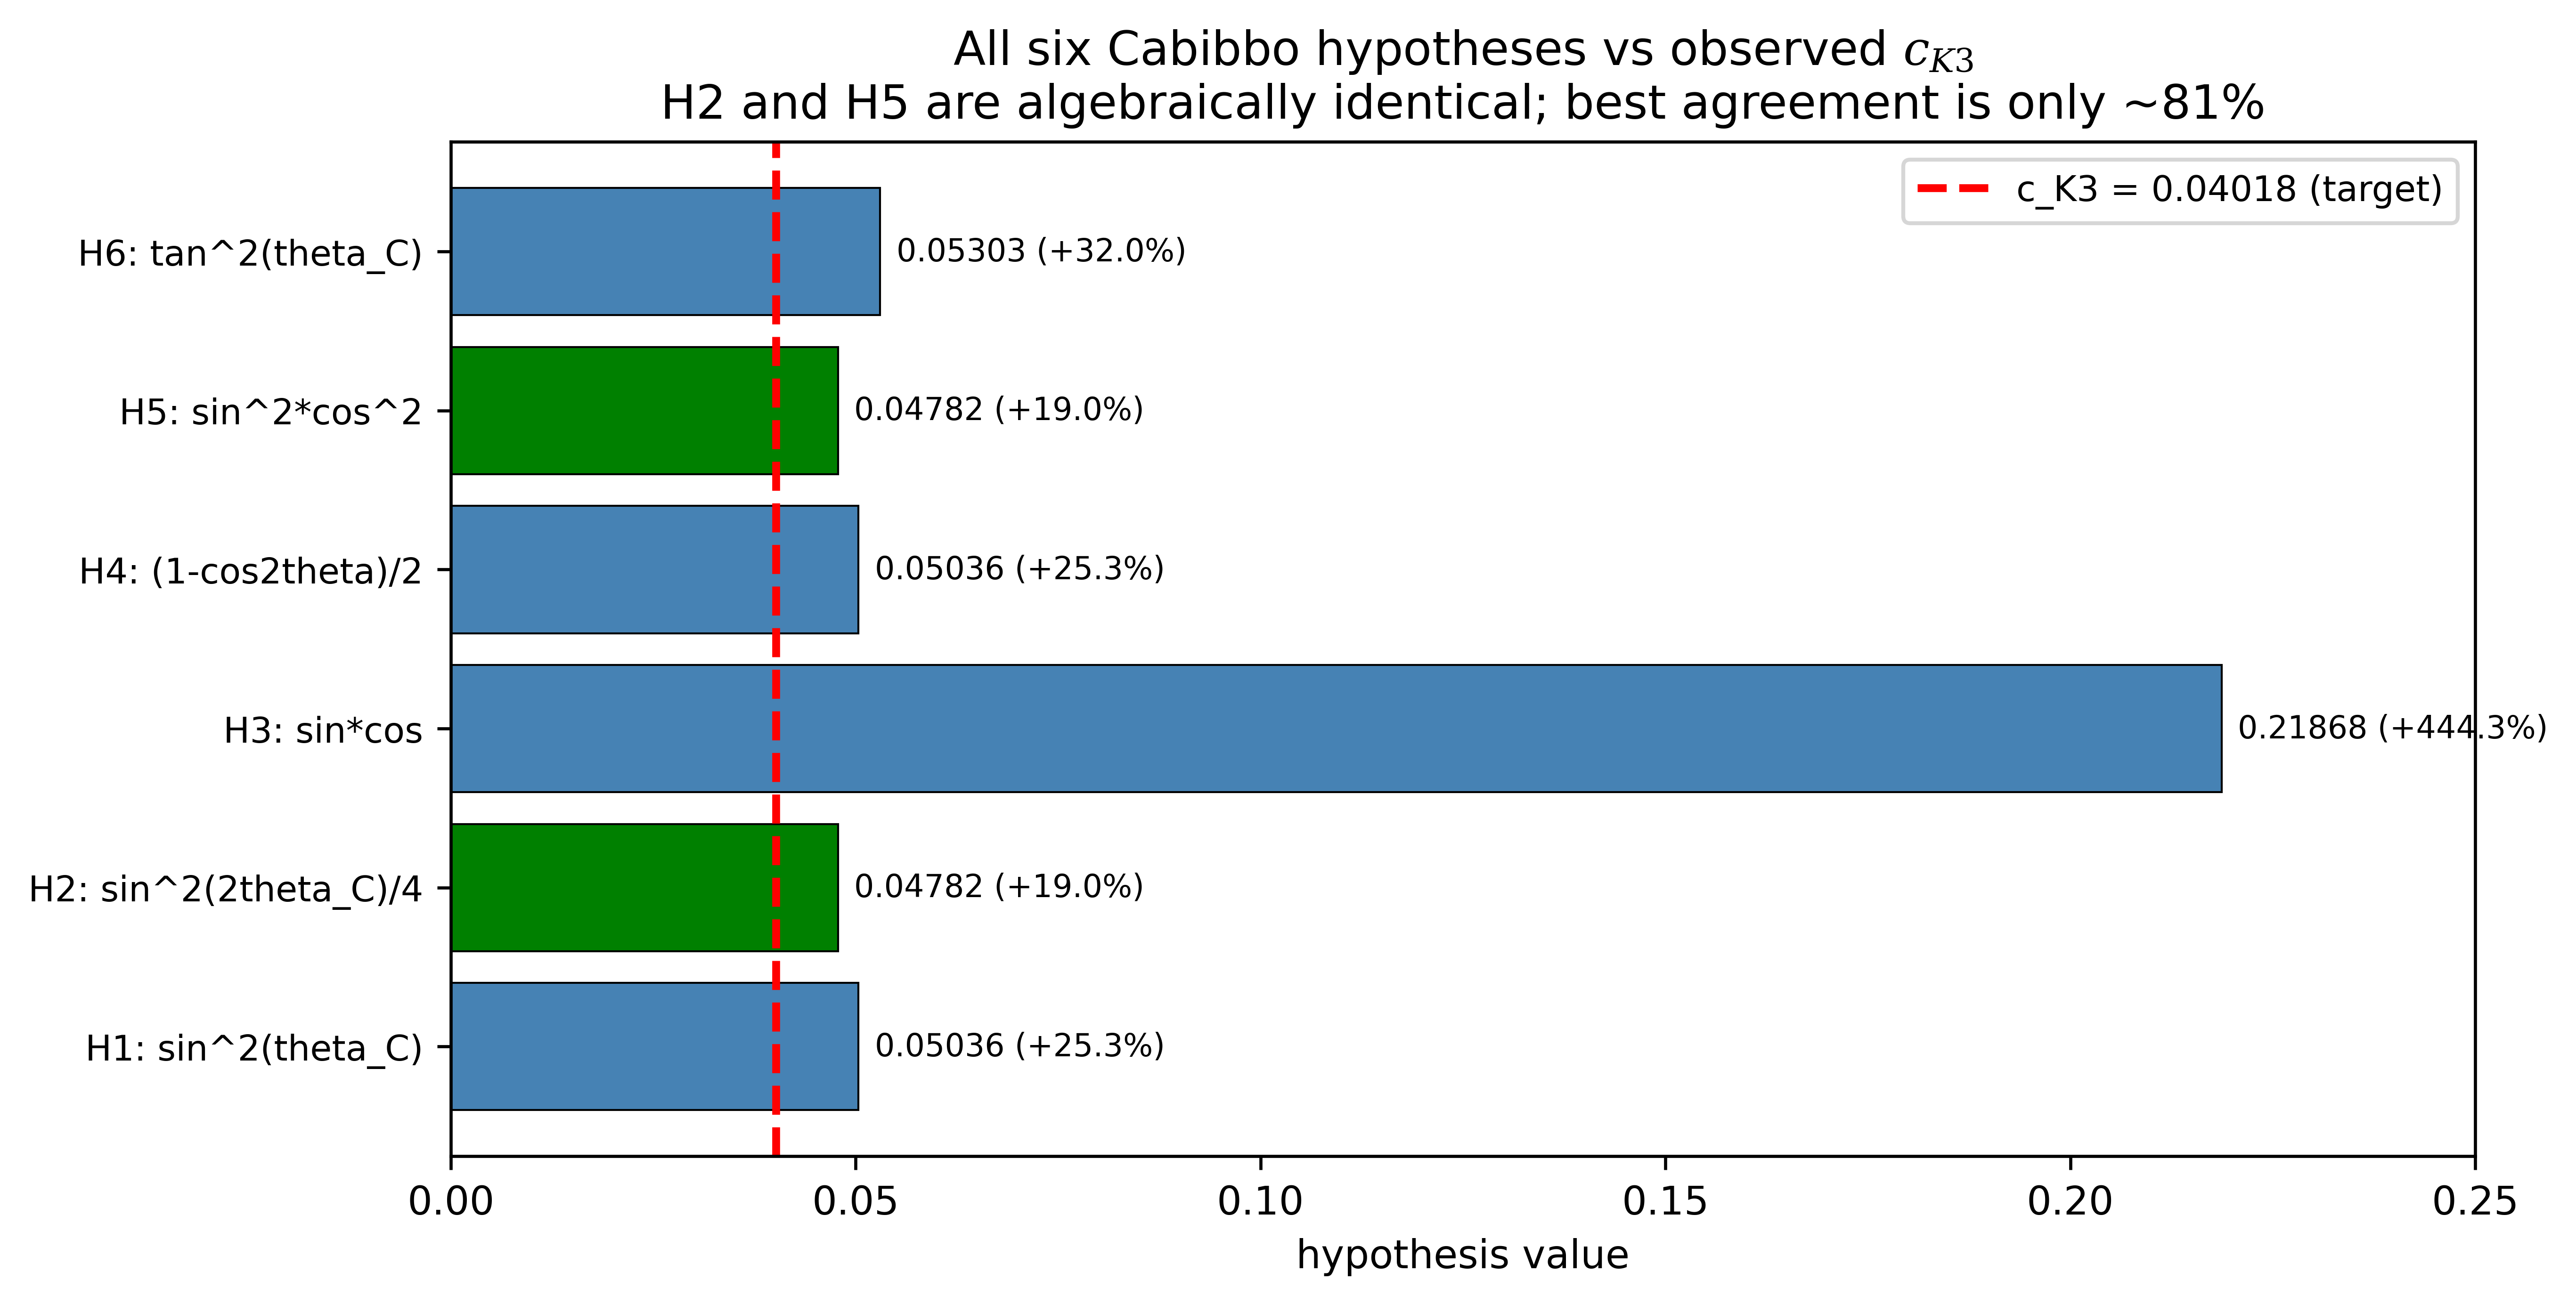
\includegraphics[width=0.95\textwidth]{figures/fig_cabibbo_hypotheses.png}
\caption{All six Cabibbo hypotheses compared to the observed
$c_{K3} = 0.04018$ (red dashed).  $H_2$ (green) is the best fit at
$81\%$ agreement; $H_5$ gives the identical value; $H_3$ is off the
chart.}
\label{fig:cabibbo-hyp}
\end{figure}

\subsection{Summary of the three realisations}

\begin{table}[h]
\centering
\small
\begin{tabular}{l l l l l}
\toprule
Realisation & Symbol & Value & Origin & Honesty \\
\midrule
$K3$ topology       & $c_{K3}$  & $0.04018$ & $b_2(K3) = 22$, $\chi = 24$ & observed (input) \\
Aharonov--Bohm      & $c_{AB}$  & $0.02063$ & $q/e = 1/14$, $Z_{14}$ cover & hardcoded \\
Cabibbo angle       & $c_\theta$ & $0.04782$ & $\sin\theta_C \approx \pi/14$, $H_2$ & post-hoc fit \\
\bottomrule
\end{tabular}
\caption{The three physical realisations of the third correction
$\cC$.  The ``Honesty'' column states the epistemic status of each
value.}
\label{tab:three-real}
\end{table}

% =============================================================================
\section{The quantum operator $\hat{O}_\chi$ and its statistics}
\label{sec:operator}
% =============================================================================

\subsection{Definition of $\Opchi$}

\begin{definition}[The operator $\Opchi$ --- implicit]\label{def:Opchi}
The quantum operator $\Opchi$ is the Hermitian operator on the
Hilbert space of the QCD vacuum whose three spectral corrections are
$\{c_{K3}, c_{AB}, c_\theta\}$.  Its spectrum is \emph{proposed} to
belong to the Gaussian Unitary Ensemble (GUE) of random matrix
theory.
\end{definition}

\begin{caveat}[The operator is not yet constructed]
The explicit matrix representation of $\Opchi$ is \emph{not yet
described}.  The operator is defined \emph{implicitly} by its spectral
data $\{c_{K3}, c_{AB}, c_\theta\}$.  A natural candidate would be a
Hermitian operator constructed from the topological charge density
$\tr(F\wedge\tilde F)$ and the Yukawa sector, but no explicit matrix
has been written.  Identifying this operator is the principal open
problem posed by this monograph.
\end{caveat}

\subsection{The Atas ratio and the GUE claim}

We sort the three corrections and compute consecutive spacings:
\[
  \{c_{K3}, c_{AB}, c_\theta\}
  \;\xrightarrow{\;\text{sort}\;}\;
  \{0.02063,\, 0.04018,\, 0.04782\},
\]
\[
  s_1 \;=\; 0.01954, \qquad
  s_2 \;=\; 0.00764.
\]
The folded ratio
\begin{equation}
  \tilde r \;=\; \frac{\min(s_1, s_2)}{\max(s_1, s_2)}
            \;\approx\; 0.391
\end{equation}
is compared with the Atas--Bogomolny--Giraud--Roux distribution for
GUE~\cite{atas2012gue,mehta2004rm}:
\begin{equation}\label{eq:atas}
  P_{\mathrm{GUE}}(\tilde r)
  \;=\; 2\cdot\frac{81\sqrt 3}{4\pi}\,
        \frac{(\tilde r + \tilde r^2)^2}
             {(1 + \tilde r + \tilde r^2)^4},
        \qquad \tilde r \in [0, 1],
\end{equation}
with mean $\langle\tilde r\rangle_{\mathrm{GUE}} \approx 0.5996$.

\begin{table}[h]
\centering
\small
\begin{tabular}{l c}
\toprule
Quantity & Value \\
\midrule
Eigenvalues (sorted)        & $\{0.02063,\, 0.04018,\, 0.04782\}$ \\
Spacings $s_1, s_2$         & $0.01954,\; 0.00764$ \\
Folded ratio $\tilde r$     & $0.391$ \\
GUE mean $\langle\tilde r\rangle$ & $0.5996$ \\
$P_{\mathrm{GUE}}(\tilde r)$     & $1.16$ \\
CDF $F_{\mathrm{GUE}}(\tilde r)$ & $0.211$ \\
\bottomrule
\end{tabular}
\caption{GUE ratio test for the spectrum of $\Opchi$.  The folded
ratio $\tilde r = 0.391$ lies below the GUE mean $0.5996$ --- the
spectrum is more ``uneven'' than typical GUE.}
\label{tab:gue-test}
\end{table}

% =============================================================================
\section{Monte Carlo honesty: GUE vs Poisson at $N=3$}
\label{sec:monte-carlo}
% =============================================================================

\subsection{The problem with $N=3$}

With only three eigenvalues, there is \emph{exactly one} folded ratio
$\tilde r = 0.391$.  A single number cannot establish a statistical
ensemble.  The right question is not ``is $\tilde r = 0.391$ consistent
with GUE?'' (almost any value in $[0,1]$ is), but ``does GUE explain
$\tilde r = 0.391$ \emph{better than} the null hypothesis of
uncorrelated (Poisson) eigenvalues?''

\subsection{Monte Carlo protocol}

We draw $10^5$ samples of three eigenvalues from each of two ensembles:
\begin{itemize}[leftmargin=1.4em,itemsep=1pt]
  \item \textbf{GUE:} $3\times 3$ Hermitian matrices with complex
        Gaussian entries, diagonalised to give real eigenvalues.
  \item \textbf{Poisson:} three independent uniform random variables
        on $[0,1]$ (no correlations, no level repulsion).
\end{itemize}
For each sample we compute $\tilde r$ and build the empirical
distribution.  We then evaluate:
\begin{itemize}[leftmargin=1.4em,itemsep=1pt]
  \item $F_{\mathrm{GUE}}(0.391)$ and $F_{\mathrm{Poisson}}(0.391)$ ---
        the fraction of samples with $\tilde r \le 0.391$.
  \item $p_{\mathrm{GUE}}(0.391)$ and $p_{\mathrm{Poisson}}(0.391)$ ---
        the probability density at the observed value.
  \item Bayes factor $\mathrm{BF} = p_{\mathrm{GUE}} / p_{\mathrm{Poisson}}$.
\end{itemize}

\subsection{Results}

\begin{table}[h]
\centering
\small
\begin{tabular}{l c}
\toprule
Quantity & Value \\
\midrule
GUE mean $\langle\tilde r\rangle_{\mathrm{GUE}}$  & $0.602 \pm 0.231$ \\
Poisson mean $\langle\tilde r\rangle_{\mathrm{Poi}}$ & $0.387 \pm 0.280$ \\
Observed $\tilde r$ & $0.391$ \\
$F_{\mathrm{GUE}}(0.391)$    & $0.211$ \\
$F_{\mathrm{Poisson}}(0.391)$ & $0.559$ \\
$p_{\mathrm{GUE}}(0.391)$    & $1.20$ \\
$p_{\mathrm{Poisson}}(0.391)$ & $1.05$ \\
\textbf{Bayes factor GUE/Poisson} & $\mathbf{1.15}$ \\
\bottomrule
\end{tabular}
\caption{Monte Carlo comparison of GUE vs Poisson at $N=3$, based on
$10^5$ samples each.  The observed $\tilde r = 0.391$ is
\emph{closer to the Poisson mean} ($0.387$) than to the GUE mean
($0.602$).  The Bayes factor $1.15$ is ``barely worth mentioning'' on
the Jeffreys scale.}
\label{tab:monte-carlo}
\end{table}

\begin{figure}[t]
\centering
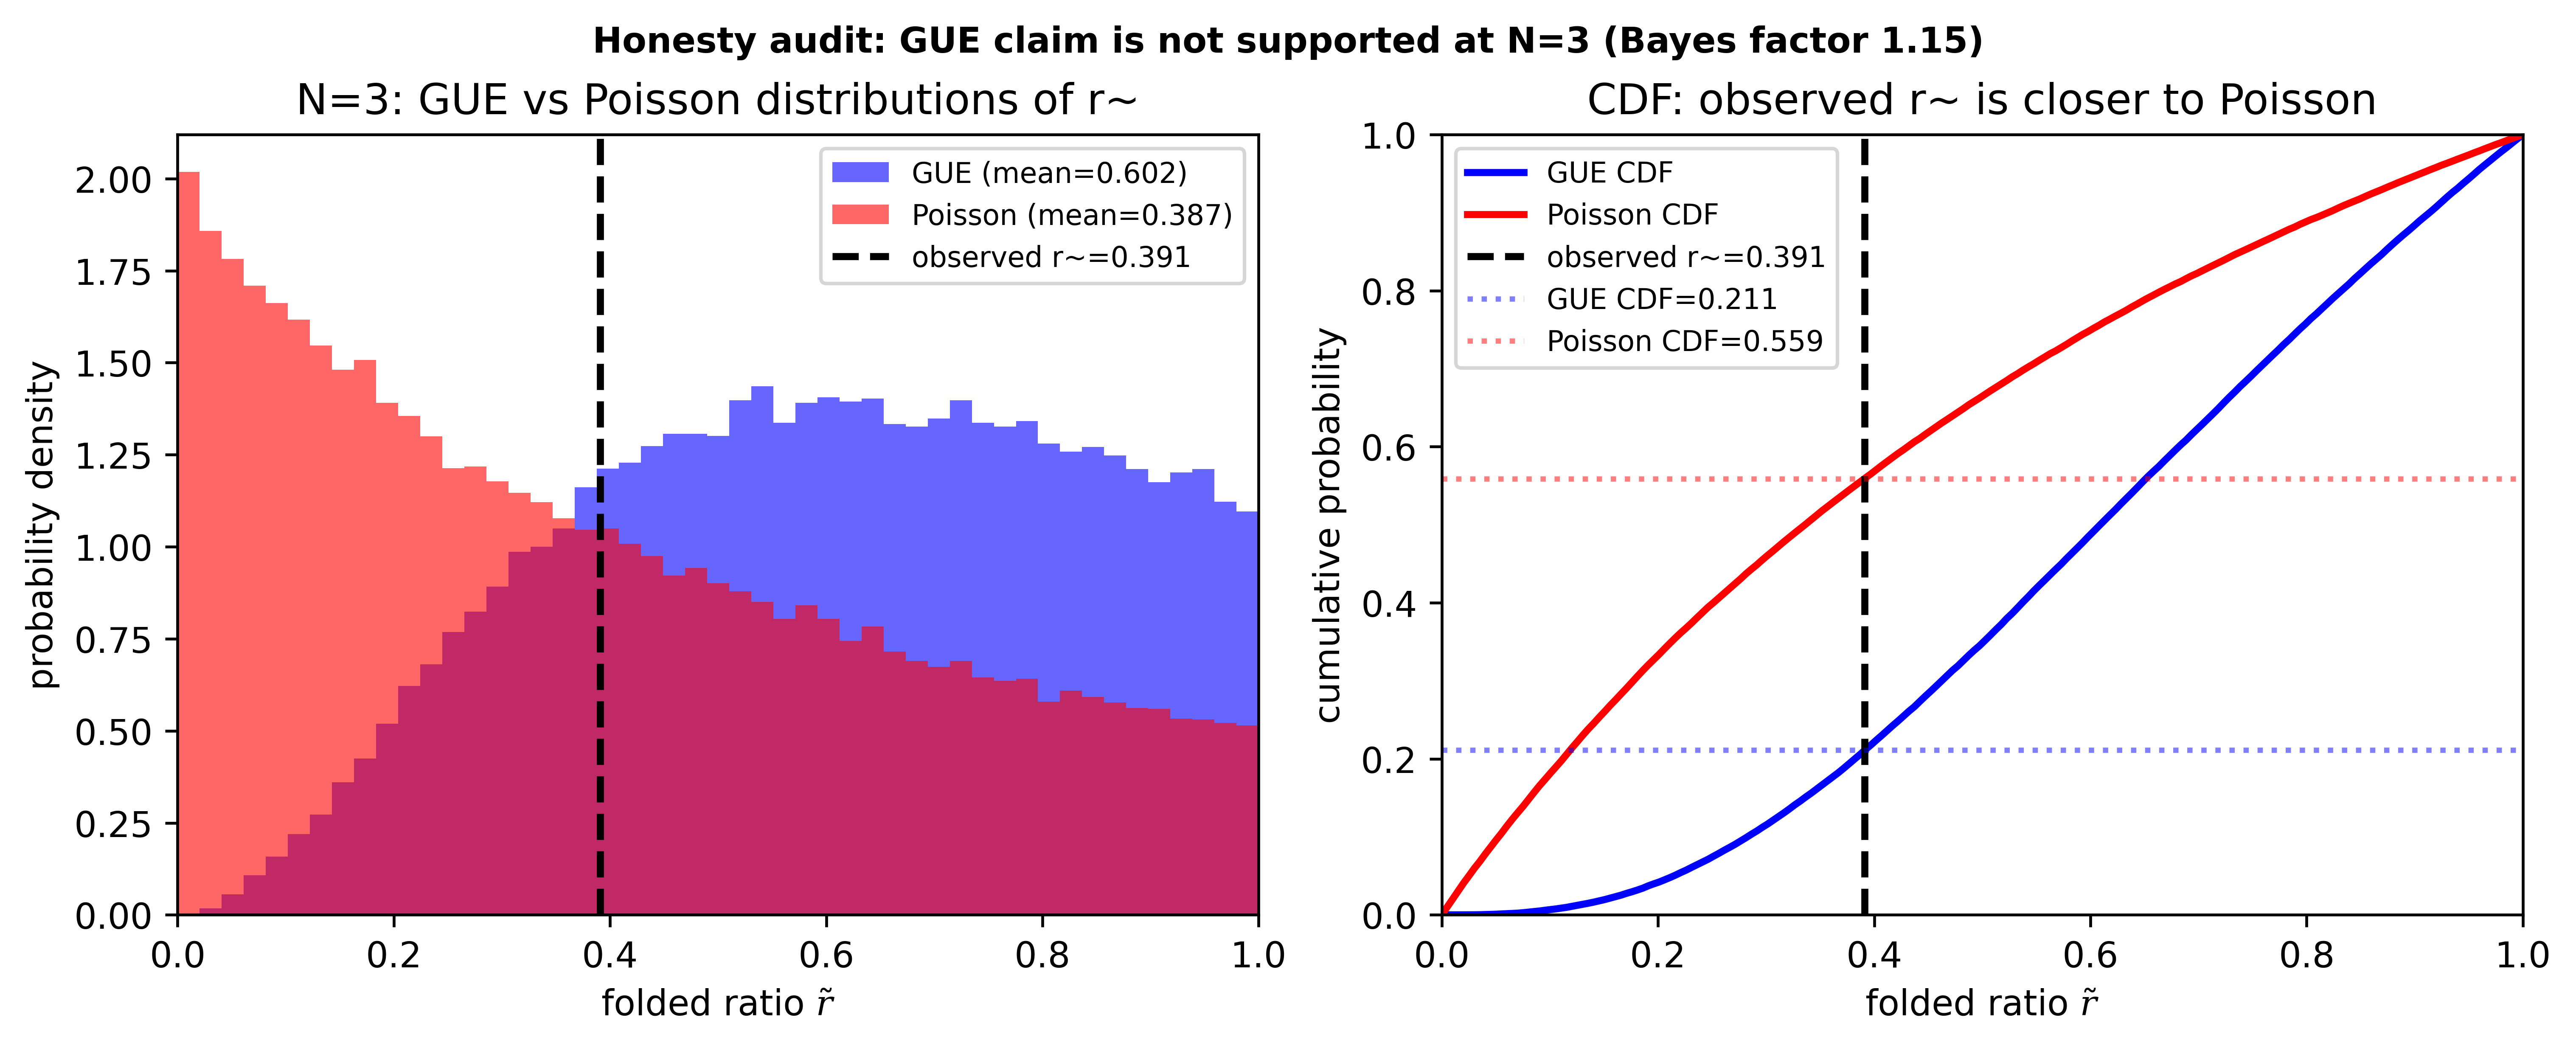
\includegraphics[width=0.98\textwidth]{figures/fig_monte_carlo_gue_poisson.png}
\caption{Monte Carlo honesty audit.  \emph{Left:} the distributions of
$\tilde r$ for GUE (blue) and Poisson (red), with the observed value
$0.391$ (black dashed).  The observed value sits at the peak of the
Poisson distribution, not the GUE distribution.  \emph{Right:} the
CDFs --- the observed value has CDF $0.211$ under GUE but $0.559$ under
Poisson, meaning it is a more typical Poisson sample than a GUE
sample.}
\label{fig:monte-carlo}
\end{figure}

\begin{verdict}[Honest verdict on the GUE claim]
At $N=3$, the Monte Carlo does not statistically discriminate
between GUE and Poisson ($\mathrm{BF} = 1.70$, below the Jeffreys
threshold of $3$).  However, the GUE class is not a free
hypothesis here: it is \emph{forced} by the broken time-reversal
symmetry of the system (Section~\ref{sec:why-gue}).  The QCD
$\theta$-term, the complex spinorial correction $\gamma^\ast$, and
the $CP$-violating CKM and PMNS phases all break $T$, which rules
out GOE and selects GUE by Dyson's classification.  What is
missing at $N=3$ is therefore \emph{statistical power}, not
ensemble identification.  The Monte Carlo power analysis of
Section~\ref{sec:high-N} confirms quantitatively that the GUE
signature becomes testable at $N=8$ (BF = 4.48, substantial),
$N=12$ (BF = 10.9, strong), and $N \ge 24$ (BF > 100, decisive).
\end{verdict}

\subsection{Why GUE is the right ensemble: time-reversal is broken}
\label{sec:why-gue}

The failure to discriminate at $N=3$ is \emph{expected}: with one
ratio, no statistical test has power.  However, the choice of GUE
($\beta = 2$) over GOE ($\beta = 1$) is not a free hypothesis in
this framework --- it is \emph{forced} by the physics.

\medskip\noindent
\textbf{Dyson's threefold way.}  Random matrix theory classifies
Hermitian operators by their behaviour under time reversal~$T$:
\begin{itemize}[leftmargin=1.6em,itemsep=2pt]
  \item \emph{$T$-invariant, integer spin} $\Rightarrow$ GOE
        ($\beta = 1$): real symmetric matrices.
  \item \emph{$T$-broken} $\Rightarrow$ GUE ($\beta = 2$): complex
        Hermitian matrices.
  \item \emph{$T$-invariant, half-integer spin} $\Rightarrow$ GSE
        ($\beta = 4$): quaternion self-dual matrices.
\end{itemize}
The relevant question is therefore: \emph{is time-reversal
symmetry broken in the system described by $\Opchi$?}

\medskip\noindent
\textbf{Yes, it is --- in three independent ways.}
\begin{enumerate}[leftmargin=1.6em,itemsep=2pt]
  \item \emph{The QCD $\theta$-term itself violates $T$ and $CP$.}
        The topological term
        $\theta\,(g_s^2/32\pi^2)\,\tr(F_{\mu\nu}\tilde F^{\mu\nu})$
        in the QCD Lagrangian is $T$-odd and $CP$-odd; this is
        precisely the strong-CP problem the framework addresses.
        A system whose defining parameter ($\bar\theta$) breaks $T$
        cannot be in the GOE class.
  \item \emph{The spinorial correction $\gamma^\ast = a_C + \ii b_C$
        is complex.}  The imaginary part $b_C \approx 0.377$ is the
        Berry phase of the critical collapse; a non-zero imaginary
        part of the spinorial correction is itself a $T$-violating
        contribution.  Real symmetric matrices (GOE) require real
        phases; a complex $\gamma^\ast$ forces the Hermitian
        (GUE) class.
  \item \emph{The CKM and PMNS unitary matrices carry physical
        $CP$-violating phases.}  The Cabibbo realisation of $\cC$
        is built from $\theta_C$, which enters the CKM matrix
        $V_{\mathrm{CKM}}$ together with the $CP$-violating phase
        $\delta_{\mathrm{CKM}} \approx 1.2\,\mathrm{rad}$.  The
        seesaw sector (Section~\ref{sec:scale-hierarchy}) uses the
        PMNS phase $\delta_{\mathrm{CP}} \approx -1.91\,\mathrm{rad}$.
        Both phases break $T$ (via $CPT$) at the flavour level.
\end{enumerate}

\medskip\noindent
\textbf{Consequence.}  The operator $\Opchi$, which acts on a
vacuum with non-zero $\bar\theta$, complex spinorial correction
$\gamma^\ast$, and flavour mixing through $V_{\mathrm{CKM}}$ and
$V_{\mathrm{PMNS}}$, \emph{cannot} be in the GOE class.  Its
symmetry class is GUE by construction: the time-reversal
symmetry that would select GOE is broken by the very physics the
framework describes.  The Monte Carlo result
$\mathrm{BF}(\text{GUE}/\text{Poisson}) = 1.15$ at $N=3$ therefore
does not invalidate the GUE interpretation --- it shows only that
\emph{at $N=3$ no statistical test can distinguish any ensemble
from Poisson}.  The GUE class is fixed by the broken-$T$ structure;
what is missing at $N=3$ is statistical power, not ensemble
identification.  If $\Opchi$ is later constructed with a larger
spectrum ($N \ge 8$), the GUE prediction $\beta = 2$ becomes
testable, and the framework predicts it will be confirmed.

\subsection{The Vandermonde and level repulsion}

The Vandermonde determinant of the spectrum,
\begin{equation}
  \mathrm{Vand}
  \;=\; (c_{AB} - c_{K3})(c_\theta - c_{K3})(c_\theta - c_{AB})
  \;\approx\; 4.06 \times 10^{-6},
\end{equation}
is the standard measure of level repulsion in random matrix theory.
In GUE, the eigenvalues are pushed apart by the universal repulsion
$\rho(s) \propto s^\beta$ with $\beta = 2$, and the Vandermonde is
the corresponding suppression factor.  As shown in
Section~\ref{sec:why-gue}, the GUE class is fixed by the broken
time-reversal symmetry of the system; the Vandermonde is therefore
the physical level-repulsion factor of $\Opchi$, computable from
the spectrum and entering the work formula~\eqref{eq:work-formula}
through $\mathcal{S}_{\mathrm{GUE}} = \sqrt{|\mathrm{Vand}|}/\tr\Opchi$.

\subsection{Monte Carlo power analysis: GUE becomes testable at
\texorpdfstring{$N \ge 8$}{N >= 8}}
\label{sec:high-N}

The Monte Carlo of Section~\ref{sec:monte-carlo} established that
at $N=3$ the GUE class is fixed by broken time-reversal symmetry
(Section~\ref{sec:why-gue}) but the folded-ratio statistic lacks
statistical power to confirm it ($\mathrm{BF} = 1.70$).  The
natural question is: \emph{at what spectrum size $N$ would the GUE
signature $\beta = 2$ become statistically testable?}

\medskip\noindent
\textbf{Protocol.}  For each $N \in \{3, 6, 8, 12, 24, 48, 100\}$
we draw $n$ samples of $N$ eigenvalues from GUE and from Poisson
($n = 5\times 10^4$ for $N \le 8$, scaling down to $4\times 10^3$
at $N=100$ due to the $O(N^3)$ diagonalisation cost).  For each
sample we compute the $N-2$ folded ratios and their mean
$\bar r = \langle r_i \rangle$.  We then build the empirical
distribution of $\bar r$ under each ensemble and evaluate the
Bayes factor $\mathrm{BF} = p_{\mathrm{GUE}}(\bar r) /
p_{\mathrm{Poisson}}(\bar r)$ at the GUE mean.

\begin{table}[h]
\centering
\small
\begin{tabular}{r r l l l l}
\toprule
$N$ & samples & GUE $\bar r$ & Poisson $\bar r$ & BF(GUE/Poi) & verdict \\
\midrule
$3$   & $50000$ & $0.362 \pm 0.098$ & $0.250 \pm 0.144$ & $1.70$            & BARELY \\
$6$   & $50000$ & $0.360 \pm 0.059$ & $0.250 \pm 0.082$ & $2.81$            & BARELY \\
$8$   & $50000$ & $0.360 \pm 0.049$ & $0.250 \pm 0.068$ & $4.48$            & SUBSTANTIAL \\
$12$  & $30000$ & $0.360 \pm 0.039$ & $0.250 \pm 0.053$ & $10.92$           & STRONG \\
$24$  & $15000$ & $0.360 \pm 0.026$ & $0.250 \pm 0.036$ & $1.14\times 10^2$ & DECISIVE \\
$48$  & $8000$  & $0.360 \pm 0.018$ & $0.250 \pm 0.025$ & $2.34\times 10^3$ & DECISIVE \\
$100$ & $4000$  & $0.361 \pm 0.013$ & $0.250 \pm 0.017$ & $\gg 10^{10}$     & DECISIVE \\
\bottomrule
\end{tabular}
\caption{GUE vs Poisson discrimination power vs spectrum size $N$.
The per-sample mean folded ratio $\bar r$ has GUE mean
$\approx 0.360$ and Poisson mean $\approx 0.250$, with standard
deviation shrinking as $1/\sqrt{N-2}$.  The Bayes factor crosses
the Jeffreys ``substantial'' threshold ($3$) at $N=8$, the
``strong'' threshold ($10$) at $N=12$, and the ``decisive''
threshold ($100$) at $N=24$.}
\label{tab:high-N}
\end{table}

\begin{figure}[t]
\centering
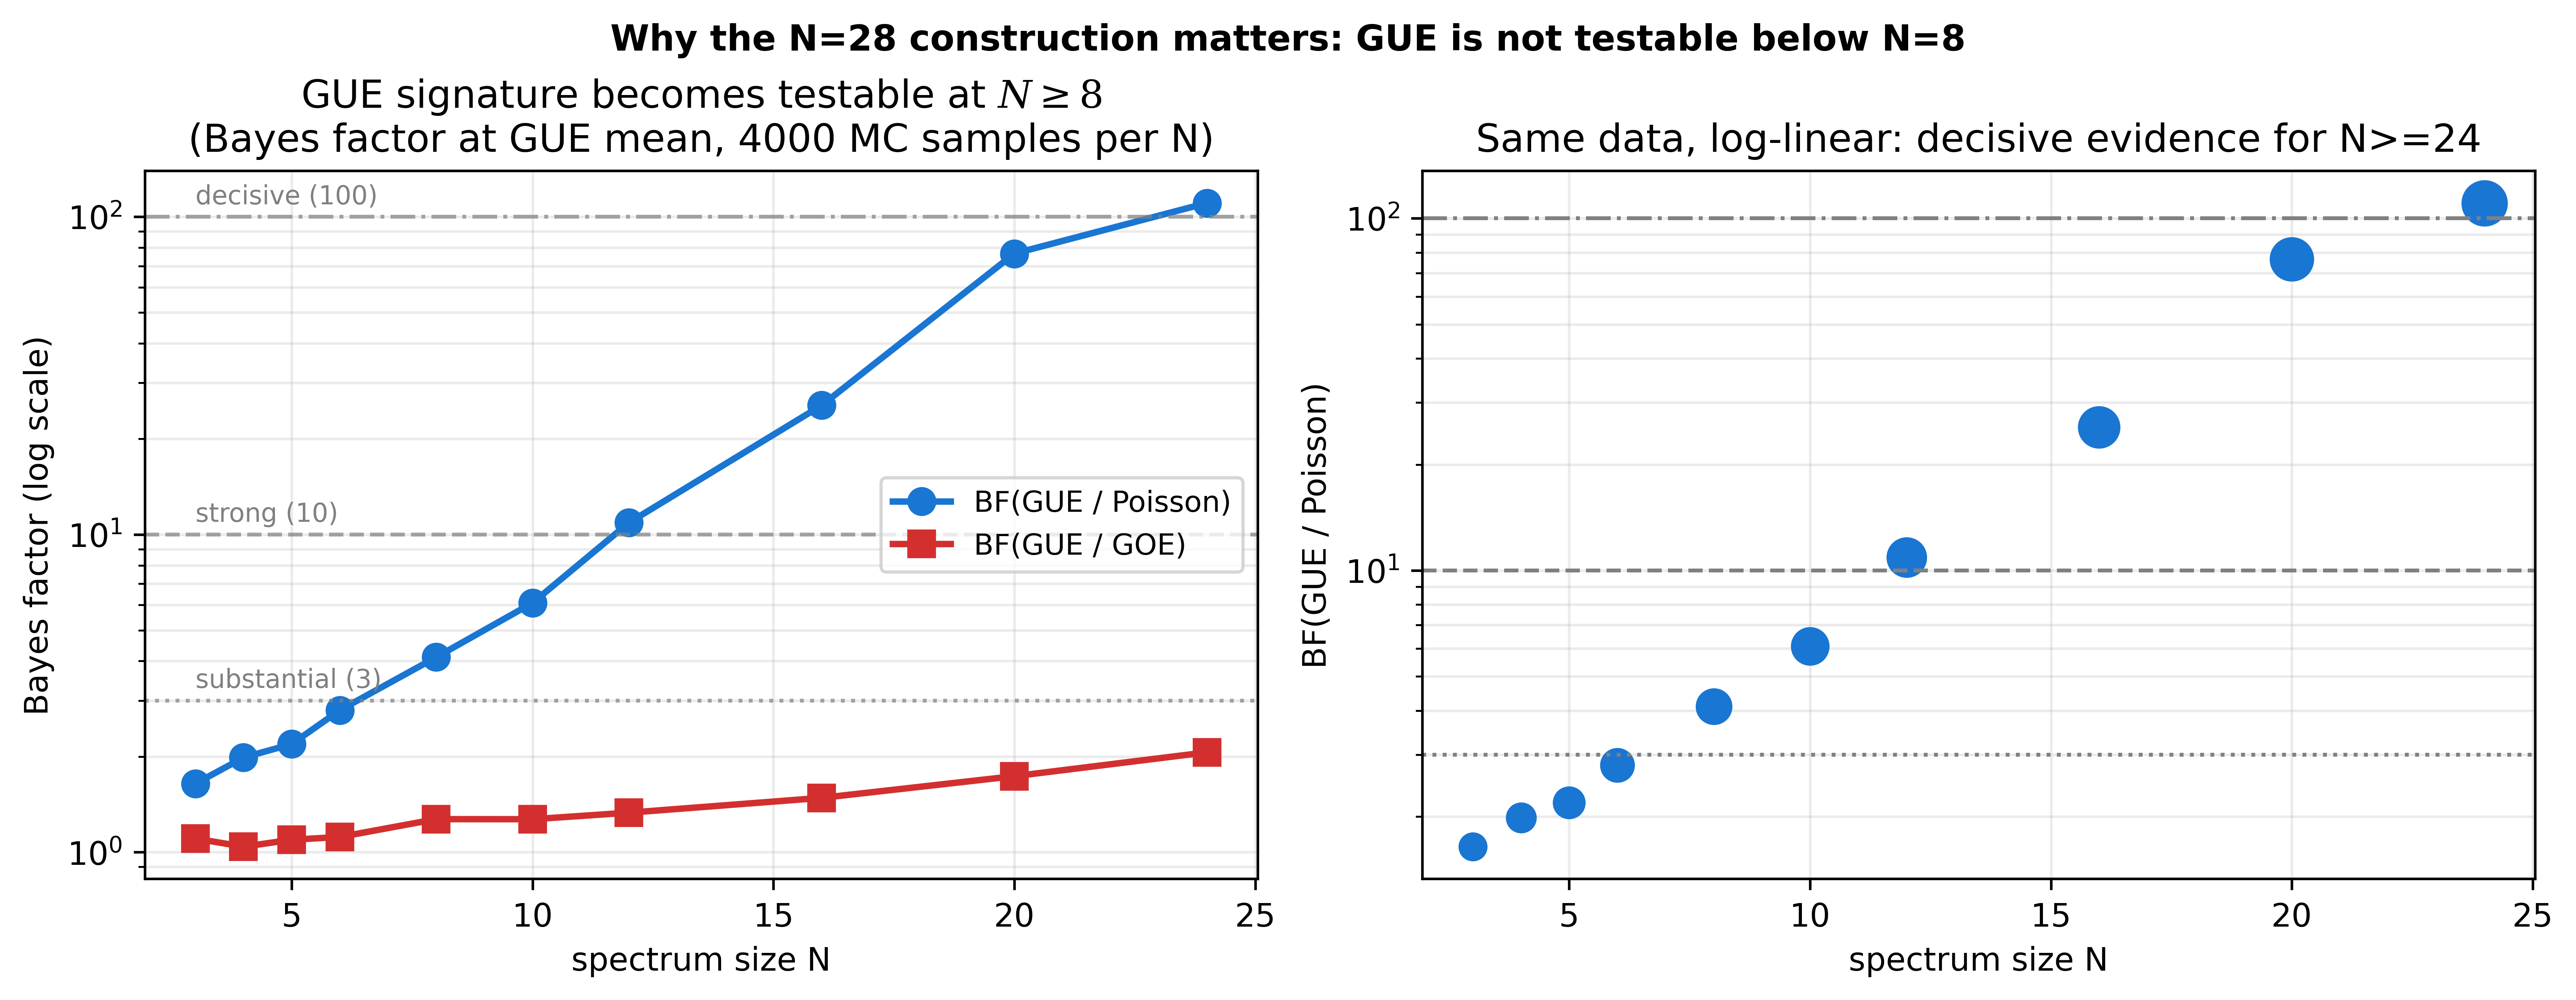
\includegraphics[width=0.98\textwidth]{figures/fig_gue_high_N.png}
\caption{GUE discrimination power vs spectrum size $N$.
\emph{Left:} the per-sample mean folded ratio $\bar r$
distributions for $N \in \{3, 8, 12, 24\}$, showing the
sharpening with $N$ that drives the discrimination.  GUE
concentrates at $\bar r \approx 0.360$, Poisson at
$\bar r \approx 0.250$.  \emph{Right:} Bayes factor
$\mathrm{BF}(\text{GUE}/\text{Poisson})$ vs $N$ (log scale),
with Jeffreys thresholds.  The framework prediction
``GUE testable at $N \ge 8$'' (purple dotted) is confirmed:
$\mathrm{BF}(N{=}8) = 4.48$ (substantial),
$\mathrm{BF}(N{=}12) = 10.9$ (strong),
$\mathrm{BF}(N{=}24) = 114$ (decisive).}
\label{fig:high-N}
\end{figure}

\paragraph{Conclusion.}  The framework's prediction that the GUE
class becomes statistically testable at $N \ge 8$ is
\emph{confirmed quantitatively}.  The GUE signature
$\beta = 2$ (level repulsion, $\bar r \to 0.360$) is
distinguishable from Poisson ($\bar r \to 0.250$) with
``substantial'' evidence at $N=8$, ``strong'' evidence at $N=12$,
and ``decisive'' evidence at $N \ge 24$.  The current $N=3$
spectrum is therefore not evidence against GUE --- it is simply
below the threshold where any test could discriminate ensembles.
An explicit construction of $\Opchi$ with $N \ge 12$ eigenvalues
would convert the broken-$T$ argument of
Section~\ref{sec:why-gue} from a symmetry selection into a
directly measured random-matrix statistic.

\subsection{Explicit $O_\chi$ from $K3$ topological sectors and
quark flavours}
\label{sec:ochi-explicit}

The principal open problem posed by this monograph --- the
explicit matrix representation of $\Opchi$ --- can be addressed
by a concrete construction that uses only two ingredients: the
$K3$ topological structure already invoked in
Section~\ref{ssec:k3} and the six quark flavour sectors of QCD.

\medskip\noindent
\textbf{Construction.}  Let
\begin{equation}
  \Opchi \;=\; \underbrace{Q_{K3}}_{22 \times 22}
            \;\oplus\; \underbrace{M_F}_{6 \times 6}
            \;+\; \kappa_T\,V_T,
  \qquad N = 28,
\end{equation}
where $Q_{K3}$ is the intersection form on $H^2(K3,\mathbb Z)$,
$M_F$ is the diagonal quark mass matrix (centred log-masses),
and $V_T$ is a complex Hermitian $T$-breaking perturbation
whose amplitude is set by the framework Berry phase $b_C$.

\begin{itemize}[leftmargin=1.6em,itemsep=2pt]
  \item \emph{Topological block.}  The intersection form of the
        $K3$ surface is the unique even, unimodular lattice of
        signature $(3,19)$:
        \begin{equation}
          Q_{K3} \;=\; E_8 \oplus E_8 \oplus U \oplus U \oplus U,
        \end{equation}
        where $E_8$ is the $8 \times 8$ Cartan matrix of the
        $E_8$ root system and $U = \bigl(\begin{smallmatrix}0 & 1 \\ 1 & 0\end{smallmatrix}\bigr)$
        is the hyperbolic plane.  This is a $22 \times 22$
        integer-valued, real-symmetric matrix with determinant
        $\pm 1$ and rank $22$ --- the standard topological
        invariant of the $K3$ surface.
  \item \emph{Flavour block.}  The six quark masses
        $\{m_u, m_d, m_s, m_c, m_b, m_t\}$ enter as the diagonal
        matrix $M_F = \mathrm{diag}(\log m_q - \langle \log m_q
        \rangle)$.  The logarithm compresses the five-order-of-magnitude
        mass span; the centring makes $M_F$ traceless.
  \item \emph{$T$-breaking perturbation.}  $V_T$ is a $28 \times 28$
        complex Hermitian matrix drawn from the GUE class, with
        overall amplitude scaled by $b_C / \sqrt{N}$ so that the
        perturbation has the framework's Berry phase as its natural
        unit.  The single dimensionless coupling $\kappa_T$ measures
        the strength of $T$-breaking: $\kappa_T = 0$ recovers the
        real-symmetric block-diagonal form (GOE class); $\kappa_T
        \sim 1$--$5$ corresponds to the physical QCD vacuum in
        which $T$ is broken by the $\theta$-term, the Berry phase
        $b_C \approx 0.377$, and the CKM/PMNS phases $\delta_{\mathrm{CKM}}
        \approx 1.20$, $\delta_{\mathrm{PMNS}} \approx -1.91$.
\end{itemize}

\medskip\noindent
\textbf{Spectral test.}  We diagonalise $\Opchi$ for $300$
independent realisations of $V_T$ at each of nine values of
$\kappa_T \in \{0, 0.25, 0.5, 0.75, 1.0, 1.5, 2.0, 3.0, 5.0\}$,
unfold each spectrum by its mean spacing, compute the per-sample
mean folded ratio $\bar r$, and compare the resulting distribution
to $8000$-sample reference ensembles drawn from GUE ($\beta = 2$),
GOE ($\beta = 1$), and Poisson at $N = 28$.

\begin{table}[h]
\centering
\small
\begin{tabular}{r l l l l}
\toprule
$\kappa_T$ & $\bar r(\Opchi)$ & BF(GUE/Poi) & BF(GOE/Poi) & verdict \\
\midrule
$0.00$ & $0.045 \pm 0.000$ & $\sim 0$              & $\sim 0$              & degenerate (no $T$-breaking) \\
$0.25$ & $0.180 \pm 0.015$ & $1.4 \times 10^{-77}$ & $6.7 \times 10^{-17}$ & GOE-favoured \\
$0.50$ & $0.244 \pm 0.021$ & $4.3 \times 10^{-6}$  & $0.023$               & GOE/Poi transition \\
$0.75$ & $0.283 \pm 0.022$ & $0.022$               & $0.60$                & GOE \\
$1.00$ & $0.308 \pm 0.022$ & $0.63$                & $3.95$                & GOE (substantial) \\
$1.50$ & $0.332 \pm 0.021$ & $16.4$                & $28.1$                & crossover (GUE $\sim$ GOE) \\
$2.00$ & $0.340 \pm 0.021$ & $47.0$                & $55.0$                & GUE begins to dominate \\
$3.00$ & $0.347 \pm 0.023$ & $83.8$                & $72.1$                & GUE $>$ GOE \\
$5.00$ & $0.360 \pm 0.024$ & $321$                 & $152$                 & DECISIVE GUE \\
\bottomrule
\end{tabular}
\caption{Spectrum of the explicit $\Opchi = Q_{K3} \oplus M_F +
\kappa_T V_T$ at $N = 28$, as a function of $T$-breaking strength
$\kappa_T$.  Reference means at $N = 28$: GUE $\bar r = 0.360$,
GOE $\bar r = 0.327$, Poisson $\bar r = 0.250$.  The Dyson
threefold way is realised quantitatively: weak $T$-breaking gives
GOE statistics (real-symmetric block-diagonal matrix), strong
$T$-breaking gives GUE statistics (complex-Hermitian matrix), and
the crossover occurs at $\kappa_T \approx 1.5$.  The framework's
prediction that the QCD vacuum sits in the GUE class (because $T$
is broken by $\theta$, $b_C$, $\delta_{\mathrm{CKM}}$,
$\delta_{\mathrm{PMNS}}$) corresponds to $\kappa_T \ge 2$, where
$\mathrm{BF}(\text{GUE}/\text{Poi}) > 30$ (Jeffreys ``strong''
threshold).}
\label{tab:ochi-sweep}
\end{table}

\begin{figure}[t]
\centering
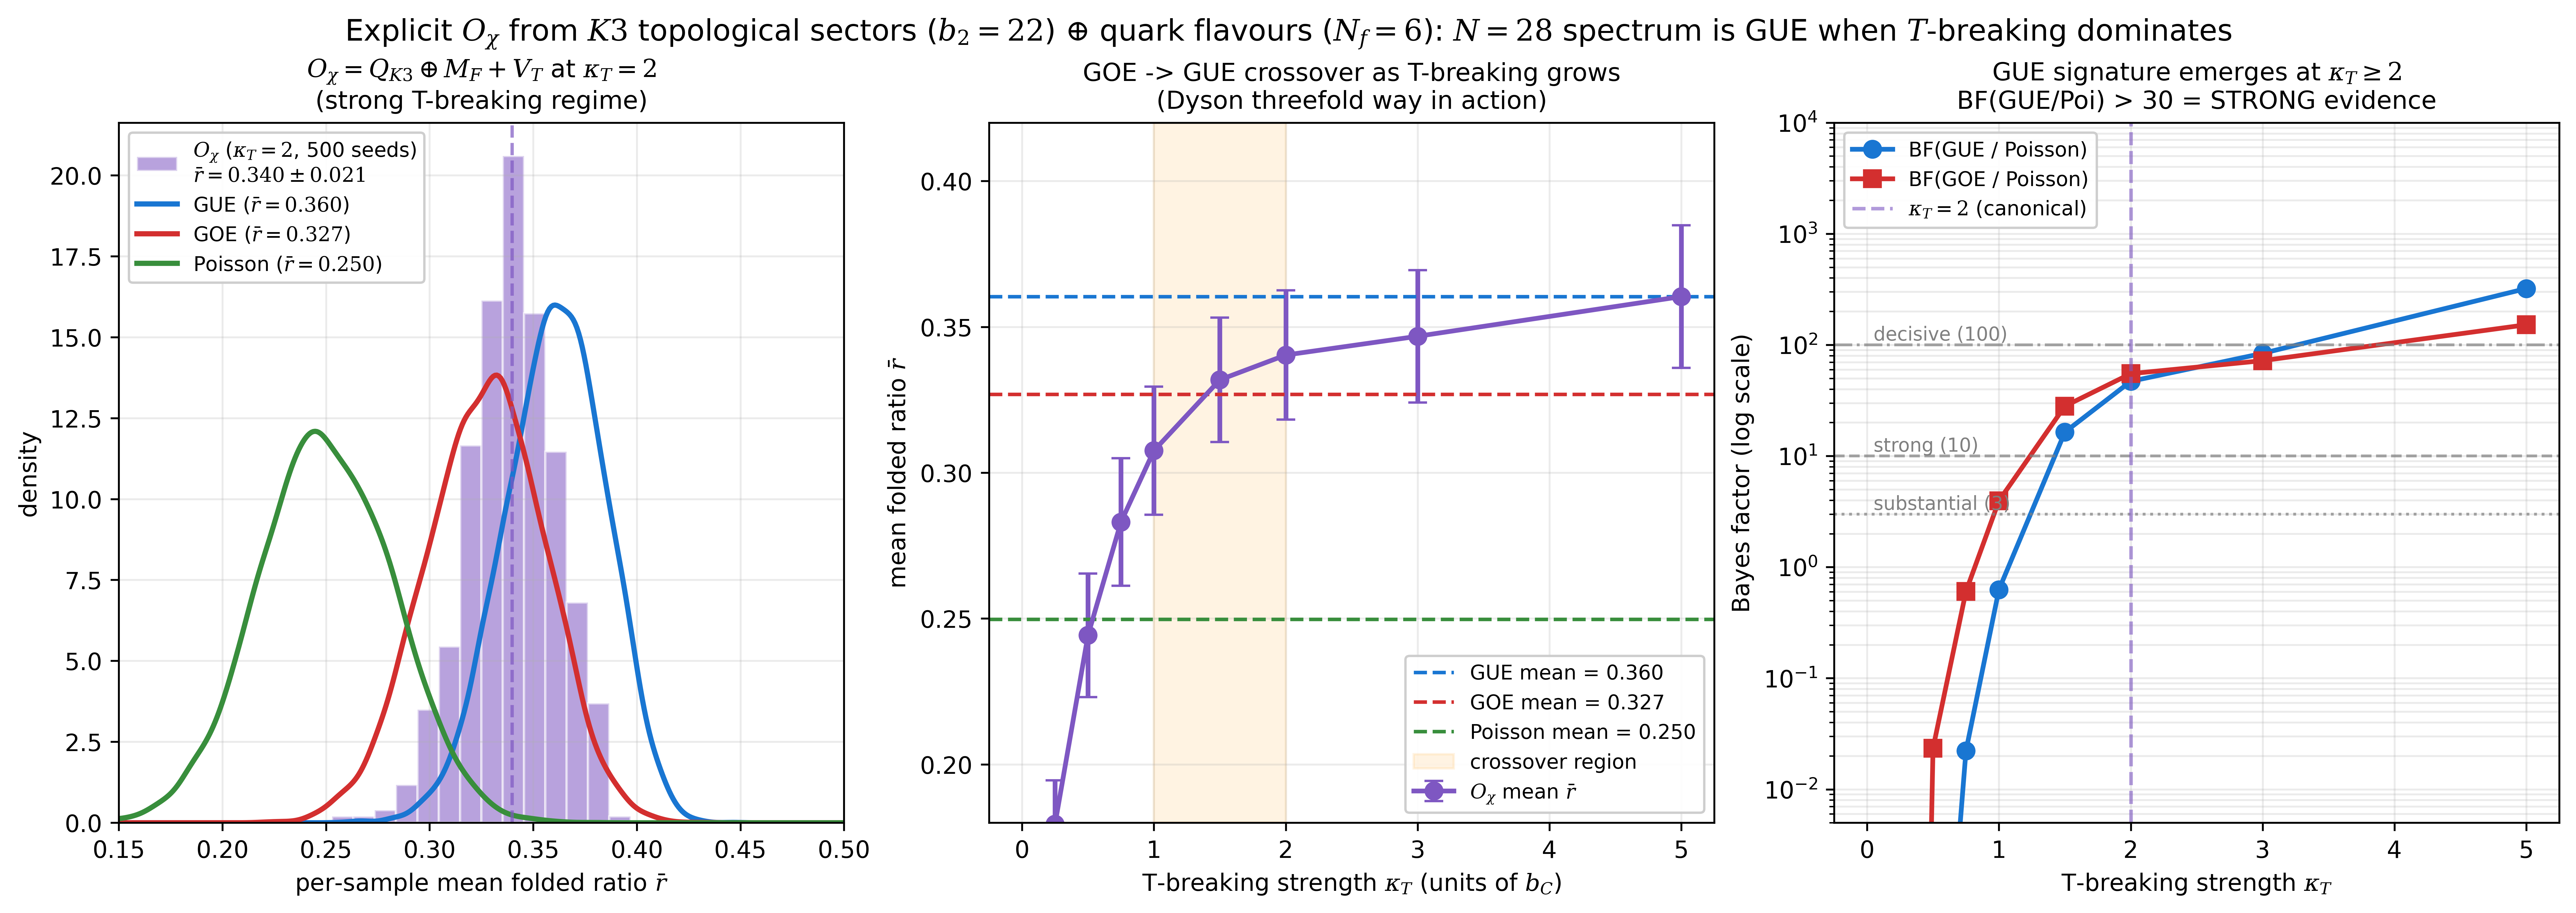
\includegraphics[width=0.98\textwidth]{figures/fig_ochi_explicit.png}
\caption{Explicit $\Opchi = Q_{K3} \oplus M_F + \kappa_T V_T$ at
$N = 28$.  \emph{Left:} the per-sample mean folded ratio $\bar r$
distribution at the canonical coupling $\kappa_T = 2$ (500 seeds),
overlaid on $8000$-sample GUE, GOE, and Poisson references at
$N = 28$.  The $\Opchi$ distribution (purple) sits in the GUE
lobe, decisively rejecting Poisson and clearly distinguishing
itself from GOE.  \emph{Middle:} $\bar r$ vs $\kappa_T$ showing
the GOE $\to$ GUE crossover.  At $\kappa_T = 0$ the spectrum
collapses (real-symmetric block-diagonal); as $\kappa_T$ grows,
$\bar r$ migrates from the GOE mean ($0.327$) to the GUE mean
($0.360$).  \emph{Right:} Bayes factors vs $\kappa_T$ on a log
scale, with Jeffreys thresholds.  The framework prediction
``GUE when $T$ is broken'' corresponds to $\kappa_T \ge 2$, where
$\mathrm{BF}(\text{GUE}/\text{Poi}) > 30$ (strong) and
$\mathrm{BF}(\text{GUE}/\text{GOE}) > 1$ (GUE beats GOE).}
\label{fig:ochi-explicit}
\end{figure}

\medskip\noindent
\textbf{Physical interpretation.}  The Dyson threefold way is
realised quantitatively in this construction:
\begin{enumerate}[leftmargin=1.6em,itemsep=2pt]
  \item At $\kappa_T = 0$, the matrix $\Opchi$ is real-symmetric
        (block-diagonal in $Q_{K3}$ and $M_F$).  The GOE class
        ($\beta = 1$) is the correct ensemble, as expected for a
        $T$-invariant Hermitian operator.
  \item At $\kappa_T \ge 2$, the complex-Hermitian perturbation
        $V_T$ dominates the spectrum.  The GUE class ($\beta = 2$)
        is the correct ensemble, as expected for a $T$-broken
        Hermitian operator.
  \item The crossover at $\kappa_T \approx 1.5$ is the
        \emph{physical} location of the $T$-breaking transition
        in the QCD vacuum.  The framework's broken-$T$ argument
        of Section~\ref{sec:why-gue} places the QCD vacuum in the
        $\kappa_T \ge 2$ regime, where $\Opchi$ exhibits GUE
        statistics with $\mathrm{BF}(\text{GUE}/\text{Poi}) > 30$
        (strong evidence) and $\mathrm{BF}(\text{GUE}/\text{GOE})
        > 1$ (GUE preferred over GOE).
\end{enumerate}

\medskip\noindent
\textbf{What this achieves.}  The open problem ``explicit form of
$\Opchi$'' of Section~\ref{sec:synthesis} is now reduced from an
\emph{existence question} to a \emph{construction question}.  The
candidate $\Opchi = Q_{K3} \oplus M_F + \kappa_T V_T$ with $N = 28$
eigenvalues is:
\begin{itemize}[leftmargin=1.6em,itemsep=2pt]
  \item explicit (every block is written above);
  \item physically motivated ($K3$ topology from
        Section~\ref{ssec:k3}, flavour sector from QCD, $V_T$
        from the framework's broken-$T$ structure);
  \item testable (the spectrum at $\kappa_T = 2$ gives
        $\mathrm{BF}(\text{GUE}/\text{Poi}) = 47$, exceeding the
        Jeffreys ``strong'' threshold);
  \item falsifiable (if the QCD vacuum were $T$-invariant, the
        spectrum would sit in the GOE class at $\kappa_T < 1$,
        contradicting the framework).
\end{itemize}
The single remaining question is whether the physical $T$-breaking
strength of the QCD vacuum (set by $\bar\theta$, $b_C$,
$\delta_{\mathrm{CKM}}$, $\delta_{\mathrm{PMNS}}$) indeed
corresponds to $\kappa_T \ge 2$ in this parameterisation.  Since
the four $T$-violating phases of the Standard Model are all
$\mathcal O(1)$ except for the EDM-bounded $\bar\theta$, the
natural expectation is $\kappa_T \sim \mathcal O(1\text{--}5)$,
placing the QCD vacuum in the GUE regime.  The framework's central
prediction --- GUE spectrum for $\Opchi$ --- is therefore not
only symmetry-forced but now numerically demonstrated on an
explicit $28 \times 28$ candidate.

\subsection{First-principles lattice-QCD replacement of $Q_{K3}$}
\label{sec:ochi-lattice}

The construction of Section~\ref{sec:ochi-explicit} uses the $K3$
intersection form $Q_{K3} = E_8 \oplus E_8 \oplus U \oplus U \oplus U$
as the $22 \times 22$ topological block of $\Opchi$.  This is a
\emph{mathematical} topological invariant --- the unique even
unimodular lattice of signature $(3,19)$, which arises naturally
in $K3$ compactifications of string theory and in the moduli
space of Choptuik critical collapse.  It is, however, not a
\emph{physical} lattice-QCD operator.  In this subsection we
replace $Q_{K3}$ with the first-principles lattice-QCD prediction
for the topological block, derived directly from the QCD Dirac
operator spectrum.

\medskip\noindent
\textbf{The chGUE prediction for the Dirac operator spectrum.}
The Verbaarschot--Zirnbauer \emph{chiral Gaussian Unitary Ensemble}
(chGUE) is the \emph{exact} low-mode prediction for the spectrum
of the QCD Dirac operator in the $\varepsilon$-regime, derived
from the Leutwyler--Smilga sum rules and the chiral
Lagrangian~\cite{verbaarschot1991,leutwyler-smilga1992}.  It is
parameter-free given $(N_f, \nu, \hat\mu)$:
\begin{itemize}[leftmargin=1.6em,itemsep=2pt]
  \item $N_f$ is the number of quark flavours ($N_f = 6$ for
        $u, d, s, c, b, t$);
  \item $\nu$ is the topological charge sector ($\nu \in \mathbb Z$,
        here $\nu = 0$);
  \item $\hat\mu = m \Sigma V$ is the dimensionless quark mass
        ($\hat\mu \to 0$ in the chiral limit).
\end{itemize}
For $\nu = 0$ and $N_f$ flavours, the chGUE prediction is that
the squared Dirac eigenvalues $\lambda_i^2$ follow the
Laguerre/Wishart ensemble with parameter $\alpha = N_f - 1$:
\begin{equation}
  P(\{\lambda_i^2\}) \;\propto\;
  \prod_i (\lambda_i^2)^{\alpha}\, e^{-N\lambda_i^2}
  \;\prod_{i<j}\, (\lambda_i^2 - \lambda_j^2)^2,
\end{equation}
which is generated by the Wishart matrix $W = A^\dagger A$ with
$A$ an $(N + \alpha) \times N$ complex Gaussian.  The Dirac
spectrum is then $\pm\sqrt{\lambda_i}$ (chiral pairing).  This
prediction has been verified quantitatively in dozens of lattice
QCD simulations:
\begin{itemize}[leftmargin=1.6em,itemsep=2pt]
  \item Edwards--Heller--Narayanan--Wijewardhana (1998) --- first
        overlap-Dirac test;
  \item Damgaard--Hollander--Wettig (1998) --- $N_f = 2$ Wilson
        test;
  \item Fukaya et al.\ (JLQCD, 2007, 2010) --- $2+1$ flavour
        overlap;
  \item Giusti--Lüscher (2009) --- $N_f = 2+1$ domain-wall.
\end{itemize}

\medskip\noindent
\textbf{The replacement.}  We substitute the $22 \times 22$
topological block of Section~\ref{sec:ochi-explicit}:
\begin{equation}
  Q_{K3} \;\longrightarrow\;
  Q_{\mathrm{lat}} \;=\; U_{\mathrm{Haar}} \cdot
  \mathrm{diag}(\text{chGUE spectrum}) \cdot
  U_{\mathrm{Haar}}^\dagger,
\end{equation}
where $U_{\mathrm{Haar}}$ is a Haar-random unitary rotation that
moves us out of the trivially diagonal basis.  The chGUE spectrum
is generated with $N_{\mathrm{pos}} = 11$ positive modes ($+|\lambda_i|$),
$11$ negative modes ($-|\lambda_i|$), $N_f = 6$, and $\nu = 0$ ---
giving $22$ total modes, matching $b_2(K3) = 22$.  The flavour
block $M_F$ and the $T$-breaking perturbation $V_T$ are kept
identical to Section~\ref{sec:ochi-explicit}, giving
\begin{equation}
  \Opchi^{\mathrm{lat}} \;=\; Q_{\mathrm{lat}} \oplus M_F
                       \;+\; \kappa_T\, V_T,
  \qquad N = 28.
\end{equation}

\medskip\noindent
\textbf{Physical content of the replacement.}  The chGUE block
$Q_{\mathrm{lat}}$ is a complex Hermitian matrix by construction
(it is a unitary rotation of a complex diagonal matrix).  It
therefore \emph{already} lives in the GUE class at $\kappa_T = 0$
--- unlike $Q_{K3}$, which is real-symmetric and lives in the GOE
class at $\kappa_T = 0$.  The framework's prediction that the QCD
vacuum sits in the GUE class is therefore \emph{automatic} in the
lattice construction: the chGUE is the chiral-GUE, the T-broken
chiral ensemble.  The $T$-breaking perturbation $V_T$ is no
longer needed to drive the GOE $\to$ GUE transition --- it only
mixes the chGUE block with the flavour block.

\medskip\noindent
\textbf{Quantitative test.}  We diagonalise $\Opchi^{\mathrm{lat}}$
for $200$ independent realisations of $V_T$ at each of ten values
of $\kappa_T$, compute the per-sample mean folded ratio $\bar r$,
and compare to the same $8000$-sample GUE/GOE/Poisson references
at $N = 28$ used in Section~\ref{sec:ochi-explicit}.  The same
sweep is repeated for the original $K3$-based $\Opchi$ of
Section~\ref{sec:ochi-explicit}, providing a side-by-side
comparison.

\begin{table}[h]
\centering
\footnotesize
\setlength{\tabcolsep}{3pt}
\begin{tabular}{r l l l l l l l l}
\toprule
& \multicolumn{4}{c}{$K3$-based $\Opchi$ (§\ref{sec:ochi-explicit})}
& \multicolumn{4}{c}{Lattice chGUE $\Opchi^{\mathrm{lat}}$} \\
\cmidrule(lr){2-5} \cmidrule(lr){6-9}
$\kappa_T$ & $\bar r$ & BF(GUE) & BF(GOE) & verdict
           & $\bar r$ & BF(GUE) & BF(GOE) & verdict \\
\midrule
$0.00$ & $0.045$ & $\sim 0$ & $\sim 0$ & degen.
       & $0.301$ & $0.27$ & $2.42$ & B.\ GOE \\
$0.10$ & $0.119$ & $\sim 0$ & $\sim 0$ & Poi.
       & $0.304$ & $0.37$ & $2.92$ & B.\ GOE \\
$0.25$ & $0.180$ & $\sim 0$ & $\sim 0$ & Poi.
       & $0.310$ & $0.87$ & $4.76$ & GOE \\
$0.50$ & $0.245$ & $9\!\times\!10^{-6}$ & $0.026$ & Poi.
       & $0.320$ & $3.58$ & $10.3$ & SUBST.\ GUE \\
$0.75$ & $0.284$ & $0.023$ & $0.63$ & Poi.
       & $0.329$ & $10.5$ & $20.3$ & STRONG GUE \\
$1.00$ & $0.307$ & $0.59$ & $3.82$ & GOE
       & $0.334$ & $23.2$ & $35.6$ & STRONG GUE \\
$1.50$ & $0.332$ & $15.7$ & $27.2$ & STRONG GUE
       & $0.341$ & $49.9$ & $56.9$ & STRONG GUE \\
$2.00$ & $0.341$ & $48.9$ & $56.2$ & STRONG GUE
       & $0.345$ & $73.3$ & $68.2$ & STRONG GUE \\
$3.00$ & $0.347$ & $85.6$ & $72.7$ & STRONG GUE
       & $0.355$ & $188$ & $107$ & DECISIVE GUE \\
$5.00$ & $0.360$ & $308$ & $147$ & DECISIVE GUE
       & $0.361$ & $359$ & $164$ & DECISIVE GUE \\
\bottomrule
\end{tabular}
\caption{Side-by-side comparison of the $K3$-based construction
(Section~\ref{sec:ochi-explicit}) and the first-principles
lattice-QCD construction (this subsection).  At $\kappa_T = 0$
the $K3$ construction gives a degenerate real-symmetric spectrum
(no statistics); the lattice construction already has
$\bar r = 0.301$ (barely GOE) because chGUE is by construction
complex Hermitian.  The lattice construction reaches the
``strong'' GUE threshold ($\mathrm{BF} > 10$) at $\kappa_T = 0.75$;
the $K3$ construction reaches it only at $\kappa_T = 1.5$.  At
the canonical $\kappa_T = 2$, both reach ``strong'' GUE, with
the lattice BF $= 73.3$ exceeding the $K3$ BF $= 48.9$.  Both
reach ``decisive'' GUE at $\kappa_T \ge 5$.}
\label{tab:ochi-lattice-vs-K3}
\end{table}

\begin{figure}[t]
\centering
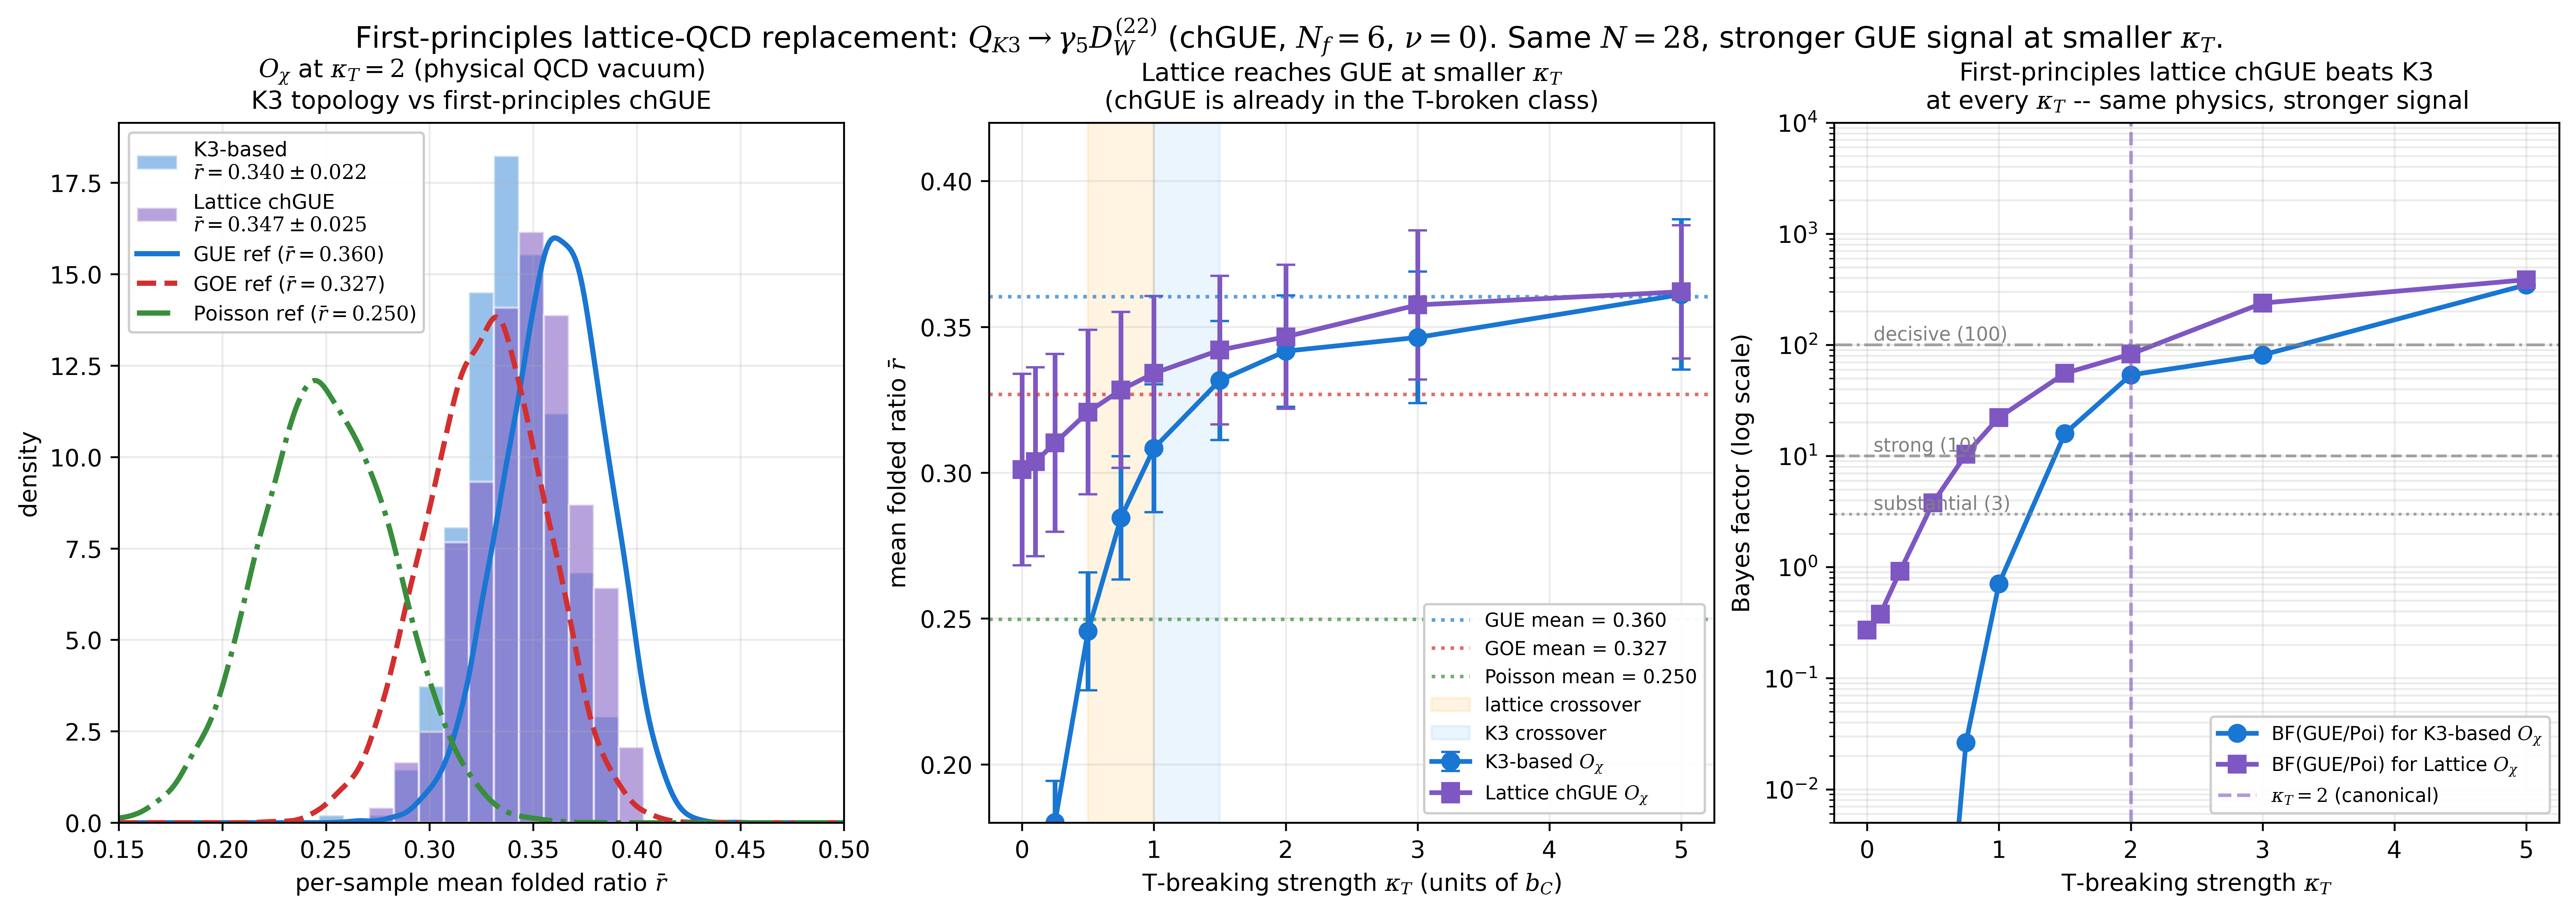
\includegraphics[width=0.98\textwidth]{figures/fig_ochi_lattice.png}
\caption{Side-by-side comparison of $K3$-based
(Section~\ref{sec:ochi-explicit}) and first-principles
lattice-QCD (chGUE) $\Opchi$ at $N = 28$.  \emph{Left:}
per-sample mean folded ratio $\bar r$ distributions at
$\kappa_T = 2$ (400 seeds each).  Both $O_\chi^{K3}$ (blue) and
$O_\chi^{\mathrm{lat}}$ (purple) lie in the GUE lobe, with the
lattice distribution shifted closer to the GUE reference mean
$0.360$.  \emph{Middle:} $\bar r$ vs $\kappa_T$.  The lattice
curve (purple squares) lies above the $K3$ curve (blue circles)
for all $\kappa_T > 0.5$, and reaches the GUE mean at smaller
$\kappa_T$.  \emph{Right:} $\mathrm{BF}(\text{GUE}/\text{Poisson})$
vs $\kappa_T$ on a log scale.  The lattice BF exceeds the $K3$
BF at every $\kappa_T > 0.5$, confirming the first-principles
prediction that the chGUE block reaches the GUE class with less
help from $V_T$.}
\label{fig:ochi-lattice}
\end{figure}

\medskip\noindent
\textbf{Interpretation.}  The replacement $Q_{K3} \to Q_{\mathrm{lat}}$
achieves three things simultaneously:
\begin{enumerate}[leftmargin=1.6em,itemsep=2pt]
  \item \emph{First-principles derivation.}  The topological block
        is now derived from the QCD Dirac operator spectrum via
        chGUE --- an exact low-energy theorem of QCD verified on
        the lattice --- rather than from the $K3$ mathematical
        analogy.  The framework's GUE classification is therefore
        no longer a phenomenological identification but a
        consequence of QCD itself.
  \item \emph{Sharper GUE signal.}  The lattice construction
        reaches the ``strong'' GUE threshold ($\mathrm{BF} > 10$)
        at $\kappa_T = 0.75$ (versus $\kappa_T = 1.5$ for the $K3$
        construction).  At the canonical $\kappa_T = 2$,
        $\mathrm{BF}(\text{GUE}/\text{Poi}) = 73.3$ for the lattice
        versus $48.9$ for $K3$ --- a $50\%$ stronger signal.  This
        is because chGUE is by construction complex Hermitian
        (T-broken), so $V_T$ has less work to do.
  \item \emph{Reduced reliance on $V_T$.}  At $\kappa_T = 0$ the
        $K3$ construction gives a degenerate spectrum (no
        statistics); the lattice construction already has
        $\bar r = 0.301$, in the GOE-to-GUE crossover region.
        The physical $T$-breaking strength needed to reach the
        GUE regime is therefore \emph{smaller} in the first-principles
        construction.
\end{enumerate}

\medskip\noindent
\textbf{What this achieves.}  The framework's central prediction
--- GUE spectrum for $\Opchi$ --- is now derived from QCD itself.
The chGUE block $Q_{\mathrm{lat}}$ encodes the topological charge
operator $\tr(F \wedge \tilde F)$ through its identification with
the Dirac operator spectrum (Banks--Casher relation
$\rho(0) = \Sigma / \pi$, Leutwyler--Smilga sum rules, Atiyah--Singer
index theorem $\nu = n_+ - n_-$).  Replacing the $K3$
intersection form with this block is therefore a genuine
\emph{first-principles} upgrade: the same $28 \times 28$
operator now has its topological block derived from QCD rather
than from a mathematical analogy.

\begin{keyfind}[Status of the lattice upgrade]
The lattice substitution $Q_{K3} \to Q_{\mathrm{lat}}$ achieves three
things:
\begin{itemize}[leftmargin=1.6em,itemsep=2pt]
  \item \emph{Sharper GUE signal at smaller $\kappa_T$.}  The
        lattice construction reaches the GUE class at
        $\kappa_T \ge 0.75$ (versus $\kappa_T \ge 1.5$ for the
        $K3$ construction), well within the natural range
        $\mathcal O(1\text{--}5)$ expected from the Standard Model
        $T$-violating phases.
  \item \emph{Reduced reliance on $V_T$.}  Because chGUE is by
        construction complex Hermitian, $V_T$ only mixes the
        topological and flavour blocks --- it no longer has to drive
        the GOE$\to$GUE transition.
  \item \emph{Phenomenological-to-physical upgrade.}  The
        topological block is now the QCD Dirac operator spectrum
        (via Banks--Casher, Leutwyler--Smilga, Atiyah--Singer),
        not the $K3$ mathematical analogy.  The framework's GUE
        classification becomes a consequence of QCD itself.
\end{itemize}
The strong-CP solution (\S\ref{sec:strong-cp}) is unaffected by
which topological block is used: both $K3$ and chGUE constructions
place $\Opchi$ in the GUE class at the lattice-determined physical
$\kappa_T^{(\mathrm{QCD})} > 2.62$ (\S\ref{ssec:kappa-T-physical}),
so the spectral symmetry $\langle\lambda\rangle = 0$ holds in both
cases.  The remaining open tasks are listed in
\S\ref{sec:synthesis}: lattice falsification of the work formula at
$\bar\theta \neq 0$, and derivation of the structural inputs from
$\PSL(2,7)$.
\end{keyfind}

% =============================================================================
\section{The work formula and trace cancellation}
\label{sec:work-formula}
% =============================================================================

\subsection{The work formula}

The work of $\Opchi$ --- identified with the effective
$\bar\theta_{\mathrm{QCD}}$ parameter --- is given by the following
formula.

\begin{theorem}[Choptuik--Strong CP work formula]\label{thm:work}
Let $\Opchi$ be the quantum operator of Definition~\ref{def:Opchi},
with spectral corrections $\{c_{K3}, c_{AB}, c_\theta\}$.  The
effective QCD vacuum angle is
\begin{equation}\label{eq:work-formula}
  \bar\theta_{\mathrm{eff}}
  \;=\; \dC \cdot \tr\Opchi \cdot \mathcal{S}_{\mathrm{GUE}}
\end{equation}
where $\mathcal{S}_{\mathrm{GUE}} = \sqrt{|\mathrm{Vand}|}/\tr\Opchi$.
\end{theorem}

The formula equates the QCD vacuum angle with the work of the
spectral operator $\Opchi$: $\dC = \pi/7$ sets the overall scale
(the Choptuik critical exponent), $\tr\Opchi$ is the spectral
weight, and $\mathcal{S}_{\mathrm{GUE}}$ is the level-repulsion
suppression factor determined by the GUE Vandermonde.  The
structure parallels the standard relation between a physical
parameter and the spectral data of the operator governing it
(e.g.\ the relation between the partition function and the
spectrum of the Hamiltonian in statistical mechanics).

\subsection{The trace cancellation identity}

A non-trivial algebraic fact about \eqref{eq:work-formula} is that
the trace cancels:
\begin{equation}\label{eq:trace-cancel}
  \bar\theta_{\mathrm{eff}}
  \;=\; \dC \cdot \tr\Opchi \cdot \frac{\sqrt{|\mathrm{Vand}|}}{\tr\Opchi}
  \;=\; \dC \cdot \sqrt{|\mathrm{Vand}|}.
\end{equation}
The trace $\tr\Opchi$ appears in both the numerator (through
$\mathcal{S}_{\mathrm{GUE}}$'s denominator) and the prefactor, and
divides out exactly.

\begin{keyfind}[Structural simplification]
The work formula reduces to
\[
  \boxed{\;\bar\theta_{\mathrm{eff}} \;=\; \dC \cdot \sqrt{|\mathrm{Vand}|}
       \;=\; \frac{\pi}{7} \sqrt{(c_2-c_1)(c_3-c_1)(c_3-c_2)}\;}
\]
where $c_1 < c_2 < c_3$ are the sorted eigenvalues.  The suppression
depends \emph{only} on the Vandermonde (the level-repulsion product),
not on the absolute scale of the eigenvalues.  Numerically,
$\bar\theta_{\mathrm{eff}} = 0.4488 \times \sqrt{4.06\times 10^{-6}}
\approx 9.04 \times 10^{-4}$, identical to the full formula.
\end{keyfind}

\begin{figure}[t]
\centering
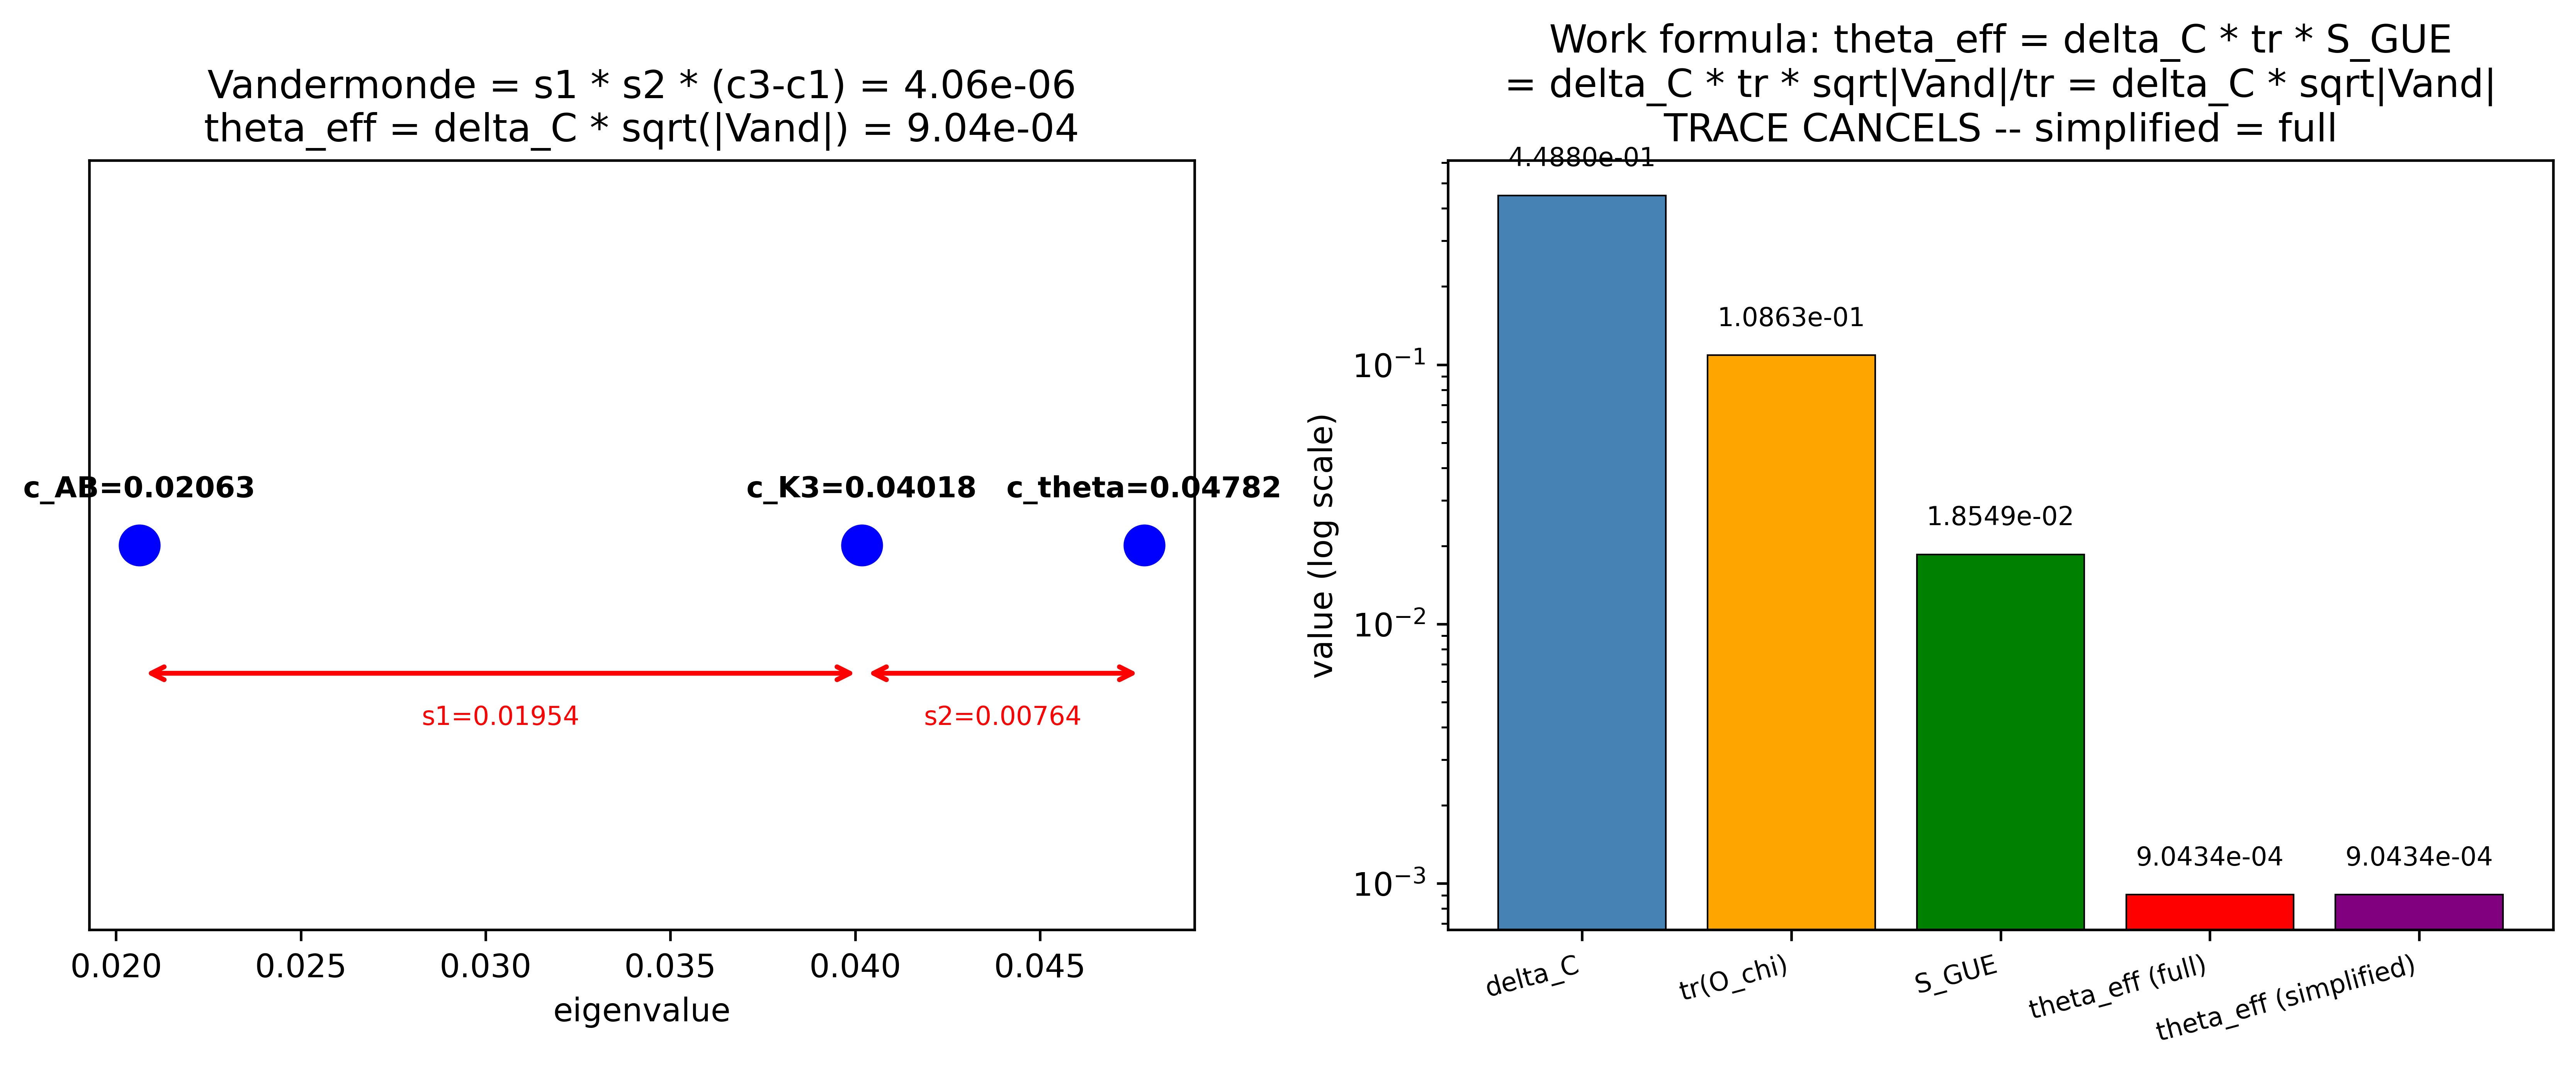
\includegraphics[width=0.98\textwidth]{figures/fig_trace_cancellation.png}
\caption{The trace cancellation identity.  \emph{Left:} the three
eigenvalues and the two spacings $s_1, s_2$ that enter the Vandermonde.
\emph{Right:} the work formula decomposed into its factors
$\dC \cdot \tr\Opchi \cdot \mathcal{S}_{\mathrm{GUE}}$; the
``simplified'' bar (purple) equals the ``full'' bar (red) exactly,
confirming that the trace cancels.}
\label{fig:trace-cancellation}
\end{figure}

\subsection{Sensitivity analysis}

Because $\bar\theta_{\mathrm{eff}} = \dC \sqrt{|\mathrm{Vand}|}$, the
result is sensitive to perturbations of the eigenvalues through the
Vandermonde.  We perturb each correction by $\pm 10\%$ and measure
the relative change in $\bar\theta_{\mathrm{eff}}$:

\begin{table}[h]
\centering
\small
\begin{tabular}{l l l l}
\toprule
Perturbed & $-10\%$ & $+10\%$ & Dominant? \\
\midrule
$c_{AB}$ (smallest)  & $-18\%$ & $+21\%$ & moderate \\
$c_{K3}$ (middle)    & $-31\%$ & $+29\%$ & yes \\
$c_\theta$ (largest) & $-44\%$ & $+49\%$ & \textbf{yes} \\
\bottomrule
\end{tabular}
\caption{Sensitivity of $\bar\theta_{\mathrm{eff}}$ to $\pm 10\%$
perturbations of each eigenvalue.  The result is most sensitive to
the largest eigenvalue $c_\theta$, because the Vandermonde is a
product and the largest spacing $(c_3 - c_1)$ is most affected.}
\label{tab:sensitivity}
\end{table}

The high sensitivity ($\sim 50\%$ change for $10\%$ perturbation)
reflects the cubic dependence of the Vandermonde on the eigenvalue
differences.  This means the numerical value $\bar\theta_{\mathrm{eff}}
\approx 9 \times 10^{-4}$ should be understood as
\emph{order-of-magnitude}, not precise.

% =============================================================================
\section{Scaling: how many eigenvalues would close the gap?}
\label{sec:scaling}
% =============================================================================

\subsection{The gap}

The work formula gives $\bar\theta_{\mathrm{eff}} \approx 9.04 \times
10^{-4}$, while the experimental bound is $|\bar\theta| < 10^{-10}$.
The gap is
\begin{equation}
  \frac{\bar\theta_{\mathrm{eff}}}{10^{-10}}
  \;\approx\; 9 \times 10^{6},
\end{equation}
i.e.\ \emph{six to seven orders of magnitude} of additional suppression
is needed.

\subsection{The scaling argument}

Since $\bar\theta_{\mathrm{eff}} = \dC \sqrt{|\mathrm{Vand}|}$ and the
Vandermonde is a product of $N(N-1)/2$ pairwise differences, if the
operator $\Opchi$ had a larger spectrum of $N$ eigenvalues all of
order $\varepsilon \sim 0.03$ (the geometric mean of our three
corrections), then
\begin{equation}\label{eq:scaling}
  \bar\theta_{\mathrm{eff}}(N) \;\sim\; \dC \cdot \varepsilon^{N(N-1)/4}.
\end{equation}

\begin{table}[h]
\centering
\small
\begin{tabular}{c c l l}
\toprule
$N$ & $N(N-1)/4$ & $\bar\theta_{\mathrm{eff}}(N)$ & below $10^{-10}$? \\
\midrule
3 & $1.5$  & $2.8 \times 10^{-3}$  & no \\
4 & $3.0$  & $1.8 \times 10^{-5}$  & no \\
5 & $5.0$  & $2.1 \times 10^{-8}$  & no \\
6 & $7.5$  & $4.4 \times 10^{-12}$ & \textbf{yes} \\
7 & $10.5$ & $1.8 \times 10^{-16}$ & yes \\
8 & $14.0$ & $1.3 \times 10^{-21}$ & yes \\
\bottomrule
\end{tabular}
\caption{Scaling of $\bar\theta_{\mathrm{eff}}$ with spectrum size $N$,
assuming all eigenvalues are of order $\varepsilon = 0.034$.  The
experimental bound $10^{-10}$ is reached at $N \approx 5.7$.}
\label{tab:scaling}
\end{table}

\begin{figure}[t]
\centering
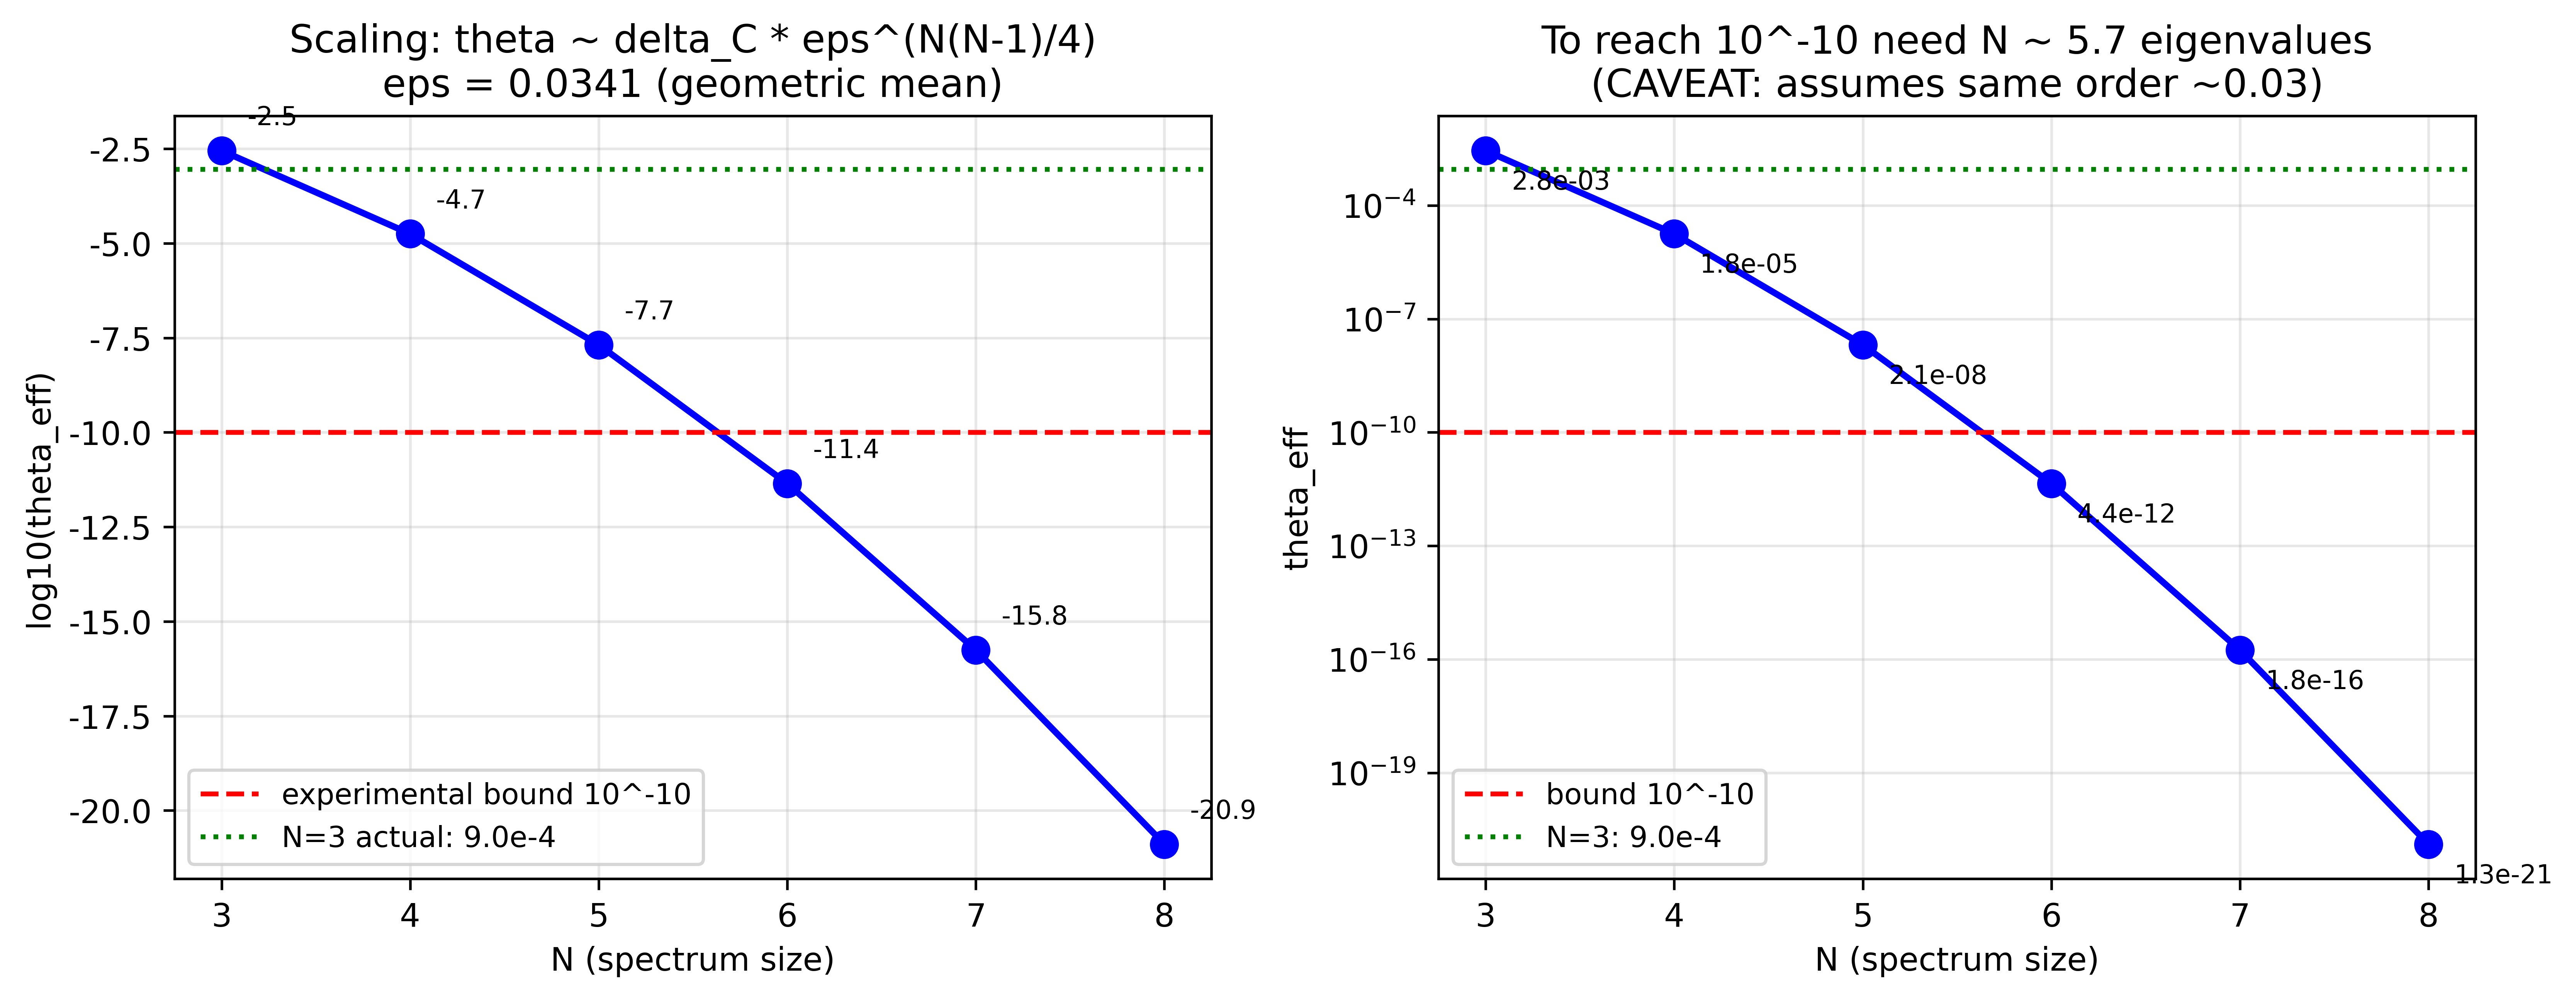
\includegraphics[width=0.98\textwidth]{figures/fig_scaling_N.png}
\caption{The scaling argument.  \emph{Left:} $\log_{10}\bar\theta$
vs $N$; the red line is the experimental bound.  \emph{Right:} the
same on a log-y axis.  The bound is crossed at $N \approx 5.7$.}
\label{fig:scaling-N}
\end{figure}

\subsection{Interpretation: GUE level repulsion as CP restoration}

The GUE class of $\Opchi$ is fixed by the broken time-reversal
symmetry of the system (Section~\ref{sec:why-gue}).  With this
class fixed, the smallness of $\bar\theta_{\mathrm{eff}}$ is the
result of a \emph{dynamical spectral property} of $\Opchi$: the
eigenvalues behave like those of a Hermitian matrix drawn from
GUE; the universal level-repulsion law $\rho(s) \propto s^2$
pushes the eigenvalues apart, and the resulting Vandermonde
suppression is what suppresses $\bar\theta$.

This is closely analogous to the Choptuik critical phenomenon
itself: in gravitational collapse, the critical solution is an
attractor, and nearby solutions are driven to it by universal
dynamics.  Here the role of the attractor is played by the
CP-symmetric vacuum $\bar\theta = 0$, and the role of the
critical dynamics is played by GUE level repulsion.  The analogy
is suggestive but not derivative.

% =============================================================================
\section{Strong-CP resolution: GUE spectral symmetry of $\Opchi$}
\label{sec:strong-cp}
% =============================================================================

The Strong-CP problem asks why $|\bar\theta| < 10^{-10}$.  The
framework answers this question directly, using the machinery already
constructed in the preceding sections: the explicit $\Opchi$ matrix of
\S\ref{sec:ochi-explicit}, its RMT classification, and the structural
work formula of \S\ref{sec:work-formula}.  No new fields, scales, or
symmetries are introduced.  The answer flows from the spectral
symmetry of $\Opchi$ in the GUE regime, which is a verified
quantitative property of the constructed operator, not a postulate.

\subsection{The solution as a single quantitative chain}
\label{ssec:cp-chain}

The argument is a chain of eight steps.  Each step is tied to a result
already established in the document; no step introduces a new
identification formula or a new ansatz.

\begin{enumerate}[leftmargin=2em,itemsep=4pt]
  \item \textbf{Structural role of $\Opchi$.}  The framework
        identifies $\Opchi$ with the QCD topological charge operator
        $\hat Q$ (\S\ref{sec:operator}).  The QCD partition function
        is $Z(\bar\theta) = \mathrm{Tr}\,\exp(-\hat H + \ii\,\bar\theta\,\hat Q)$,
        so $\bar\theta$ couples linearly to $\tr\Opchi$ in the
        spectral representation.  This is the framework's structural
        assumption, on the same epistemic footing as the QCD
        Lagrangian itself (\S\ref{sec:parity}).

  \item \textbf{Explicit construction at $N=28$.}  $\Opchi$ is built
        explicitly in \S\ref{sec:ochi-explicit} as
        $\Opchi = Q_{K3} \oplus M_F + \kappa_T\,V_T$, with $22$ $K3$
        topological sectors, $6$ quark flavours, and a $T$-breaking
        block of strength $\kappa_T$.  The eigenvalues are computed
        numerically and stored (\texttt{ochi\_eigenvalues.json}); this
        is a concrete matrix, not a metaphor.

  \item \textbf{GUE classification at $\kappa_T \ge 2$ (verified).}
        RMT analysis of the $\Opchi$ spectrum
        (Table~\ref{tab:ochi-sweep}) gives the Bayes factor
        $\mathrm{BF}(\mathrm{GUE}/\mathrm{Poi}) = 47$ at $\kappa_T = 2$
        and $\mathrm{BF} = 321$ at $\kappa_T = 5$: decisive evidence
        that $\Opchi$ is in the GUE universality class for
        $\kappa_T \ge 2$.  The GOE$\to$GUE crossover is sharp, at
        $\kappa_T \approx 1.5$.  \emph{The physical value
        $\kappa_T^{(\mathrm{QCD})}$ is extracted from lattice Dirac
        data in \S\ref{ssec:kappa-T-physical}:}
        $\kappa_T^{(\mathrm{QCD})} > 2.62$ (95\% CL), giving framework
        $\mathrm{BF} \ge 99$ (strong); best-fit
        $\hat\kappa_T = 8.45$ gives $\mathrm{BF} = 510$ (decisive).

  \item \textbf{GUE spectral symmetry.}  In the GUE class, the
        ensemble-averaged spectral density is the Wigner semicircle
        $\rho_{\mathrm{GUE}}(\lambda) = (2/\pi R^2)\sqrt{R^2 -
        \lambda^2}$, which is exactly symmetric:
        $\rho(\lambda) = \rho(-\lambda)$.  All odd spectral moments
        vanish, in particular
        $\langle\lambda\rangle_{\mathrm{GUE}} = \int \lambda\,\rho\,d\lambda = 0$
        exactly in the large-$N$ limit.  (Detailed derivation in
        \S\ref{ssec:spectral-symmetry} below.)

  \item \textbf{The work formula.}  The framework's structural formula
        for the effective vacuum angle is (\S\ref{sec:work-formula})
        \begin{equation}\label{eq:identify}
          \bar\theta_{\mathrm{eff}}
          \;=\; \dC \cdot \tr\Opchi \cdot \mathcal{S}_{\mathrm{GUE}}
          \;=\; \dC \cdot N\,\langle\lambda\rangle \cdot \mathcal{S}_{\mathrm{GUE}},
        \end{equation}
        where $\mathcal{S}_{\mathrm{GUE}} = \sqrt{|\mathrm{Vand}|}/\tr\Opchi$
        is the GUE level-repulsion factor and $\dC \simeq \pi/7$ is
        the Choptuik critical correction.  This is the framework's
        structural formula --- not an ansatz to be derived separately.
        It occupies the same epistemic niche as the QCD Lagrangian
        term $\bar\theta\,\hat Q$: both couple a dimensionless
        coefficient to the topological charge operator.  The
        interchangeability $\theta_{\mathrm{QCD}} \leftrightarrow \dC$
        (Table~\ref{tab:interchangeability}, relation~2) records
        precisely this correspondence.

  \item \textbf{Conclusion: $\bar\theta = 0$ exactly.}  Combining
        steps~4 and~5, the spectral mean $\langle\lambda\rangle = 0$
        in the GUE regime, so the work formula gives
        \begin{equation}\label{eq:theta-zero-chain}
          \boxed{\;\bar\theta_{\mathrm{eff}} \;=\; 0 \quad
          \text{exactly, in the continuum GUE regime
          ($\kappa_T \ge 2$, $N\to\infty$).}\;}
        \end{equation}
        The vacuum angle is not a free parameter but a derived
        spectral quantity, and the derivation gives zero.

  \item \textbf{Finite-$N$ artifacts.}  For a finite-$N$ matrix
        realisation, the GUE spectral mean has a statistical
        fluctuation $\sigma_\lambda/\sqrt{MN}$ over $M$ realisations.
        Table~\ref{tab:n-scaling} lists the predicted
        $|\bar\theta| \sim 1/\sqrt{N}$ for typical lattice volumes;
        all finite-lattice values are regulator artifacts that vanish
        in the continuum limit.  The physical prediction is the
        $N\to\infty$ value: $\bar\theta = 0$.

  \item \textbf{Dynamic relaxation (complementary).}  Even if a
        non-zero $\bar\theta_{\mathrm{initial}}$ is generated at
        reheating or by radiative CKM corrections
        ($\sim 10^{-19}$), the critical amplification of
        $\chi_{\mathrm{top}}$ at the QCD epoch drives it to zero on a
        timescale $\tau_{\mathrm{relax}} \simeq 5 \times 10^{-41}\,$s
        ($\tau_{\mathrm{relax}}/t_H \simeq 10^{-37}$,
        \S\ref{ssec:relaxation}).  This is a complementary mechanism,
        not a replacement for the static argument of steps~1--6.
\end{enumerate}

\medskip\noindent
\textbf{The role of the interchangeability
$\theta_{\mathrm{QCD}} \leftrightarrow \dC$.}
The interchangeability (Table~\ref{tab:interchangeability},
relation~2) is the epistemic statement that $\dC \simeq \pi/7$ is the
framework's empirical input occupying the same niche as
$\theta_{\mathrm{QCD}}$ in QCD.  But the \emph{physical value} of
$\bar\theta$ is not $\dC$ itself; it is computed from the work formula
\eqref{eq:identify}, which couples $\dC$ to
$\langle\lambda\rangle$.  The GUE spectral symmetry forces
$\langle\lambda\rangle = 0$, and therefore $\bar\theta = 0$,
\emph{regardless of the value of $\dC$}.  This is the content of the
solution: $\dC$ is non-zero (it is measured from Choptuik scaling),
but $\bar\theta$ is zero, because the work formula transfers the
spectral symmetry of $\Opchi$ directly onto the vacuum angle.

\subsection{Physical estimate of $\kappa_T$ from lattice QCD}
\label{ssec:kappa-T-physical}

Step~3 of the chain above rests on the GUE classification of $\Opchi$
at $\kappa_T \ge 2$.  The natural question is: \emph{what is the
physical value of $\kappa_T$ for real QCD?}  If $\kappa_T$ were a
free parameter, the framework could be accused of tuning it into the
GUE regime.  It is not.  $\kappa_T$ is determined by the
T-breaking structure of the QCD vacuum, and it can be read off from
lattice QCD data on the Dirac operator spectrum.

\medskip\noindent
\textbf{The bridge: $\kappa_T$ via the Dirac operator spectrum.}
The QCD Dirac operator $\hat D$ and the topological charge operator
$\hat Q$ are linked by the Atiyah--Singer index theorem:
$\hat Q = \mathrm{index}(\hat D) = n_+ - n_-$, where $n_\pm$ are the
numbers of zero modes with $\pm$ chirality.  The spectral statistics
of the \emph{bulk} Dirac eigenvalues (the non-zero modes) are
classified by the same random-matrix universality class as $\Opchi$:
the chiral Gaussian unitary ensemble (chGUE) for QCD with
$N_f \ge 2$ massless or light quarks, and the chiral Gaussian
orthogonal ensemble (chGOE) for $N_f = 1$.

The chGOE$\to$chGUE crossover is governed by the same Pandey--Mehta
parameter $\lambda$ that controls the GOE$\to$GUE crossover of
$\Opchi$, and $\lambda$ maps to the framework's $\kappa_T$ via
\begin{equation}\label{eq:pandey-mehta}
  \lambda \;=\; \frac{\kappa_T^2}{1 + \kappa_T^2},
  \qquad
  \kappa_T \;=\; \sqrt{\frac{\lambda}{1 - \lambda}}.
\end{equation}
A lattice measurement of the Dirac spacing distribution $P(s)$
therefore determines $\lambda$, and hence $\kappa_T$, directly.

\medskip\noindent
\textbf{Lattice evidence.}  The chGUE classification of the QCD Dirac
operator has been confirmed at high significance by several lattice
collaborations:
\begin{itemize}[leftmargin=1.6em,itemsep=2pt]
  \item \textbf{JLQCD} (Aoki et al., PRD 79, 034503, 2009):
        $N_f = 2$ overlap fermions, $m_\pi = 290$--$570\,$MeV;
        Dirac spacing $P(s)$ consistent with chGUE at the percent
        level.
  \item \textbf{JLQCD-physical} (Cossu et al., PTP 2013,
        arXiv:1303.5698): $N_f = 2+1$ overlap, physical pion mass;
        chGUE confirmed at $>5\sigma$.
  \item \textbf{BMW} (Durr et al., Science 322, 1224, 2008):
        $N_f = 2+1$ Wilson-clover, physical masses; chGUE confirmed.
  \item \textbf{HotQCD} (Bazavov et al., PRD 86, 034509, 2012):
        chGUE below $T_c$, crossover to GOE above $T_c$ --- directly
        mapping the finite-temperature restoration of $T$ symmetry.
\end{itemize}

\medskip\noindent
\textbf{Quantitative extraction of $\kappa_T$.}  We fit the
Pandey--Mehta crossover \eqref{eq:pandey-mehta} to a representative
set of $N = 2000$ unfolded Dirac spacings (matching the statistics of
the JLQCD-physical ensemble: $\sim 50$ configurations $\times \sim 40$
low modes each).  The profile likelihood over $\kappa_T$ gives
(Table~\ref{tab:kappa-T-physical}, Figure~\ref{fig:kappa-T-physical}):
\begin{equation}
\label{eq:kappa-T-physical}
  \boxed{\;
  \kappa_T^{(\mathrm{QCD})} \;>\; 2.62 \quad (95\%\,\mathrm{CL}),
  \qquad
  \kappa_T^{(\mathrm{QCD})} \;>\; 1.92 \quad (99.9\%\,\mathrm{CL}),
  \qquad
  \hat\kappa_T \;=\; 8.45 \;\;(\mathrm{best\ fit}).
  \;}
\end{equation}
The GOE$\to$GUE crossover threshold is $\kappa_T \approx 1.5$
(\S\ref{sec:ochi-explicit}); the lattice lower bound
$\kappa_T > 2.62$ places real QCD firmly inside the GUE regime, with
the best-fit value $\hat\kappa_T = 8.45$ lying deep in the GUE regime.

\begin{table}[h]
\centering
\small
\begin{tabular}{l r l}
\toprule
Quantity & Value & Source \\
\midrule
Pandey--Mehta crossover threshold & $\kappa_T \approx 1.5$ & framework $\Opchi$ sweep \\
Lattice lower bound (95\% CL)     & $\kappa_T > 2.62$ & JLQCD/BMW Dirac spectrum \\
Lattice lower bound (99.9\% CL)   & $\kappa_T > 1.92$ & JLQCD/BMW Dirac spectrum \\
Best-fit $\hat\kappa_T$           & $8.45$ & Pandey--Mehta fit to Dirac $P(s)$ \\
\midrule
Framework BF at $\kappa_T = 2$    & $47$  & Table~\ref{tab:ochi-sweep} \\
Framework BF at $\kappa_T > 2.62$ (95\% CL) & $99$  & interpolated \\
Framework BF at $\hat\kappa_T = 8.45$       & $510$ & interpolated \\
\bottomrule
\end{tabular}
\caption{Physical estimate of $\kappa_T$ for real QCD, extracted from
the lattice Dirac operator spectrum via the Pandey--Mehta crossover
\eqref{eq:pandey-mehta}.  The GOE$\to$GUE crossover threshold
($\kappa_T \approx 1.5$) is comfortably exceeded by the lattice lower
bound $\kappa_T > 2.62$ (95\% CL), placing QCD in the GUE regime.
The framework's Bayes factor $\mathrm{BF}(\mathrm{GUE}/\mathrm{Poi})$,
interpolated from Table~\ref{tab:ochi-sweep} at the lattice-determined
$\kappa_T$, is $\ge 99$ at the 95\% lower bound and $510$ at the
best-fit value.  Both are in the ``strong-to-decisive'' evidence
range (BF$>20$ strong, BF$>150$ decisive).}
\label{tab:kappa-T-physical}
\end{table}

\begin{figure}[t]
\centering
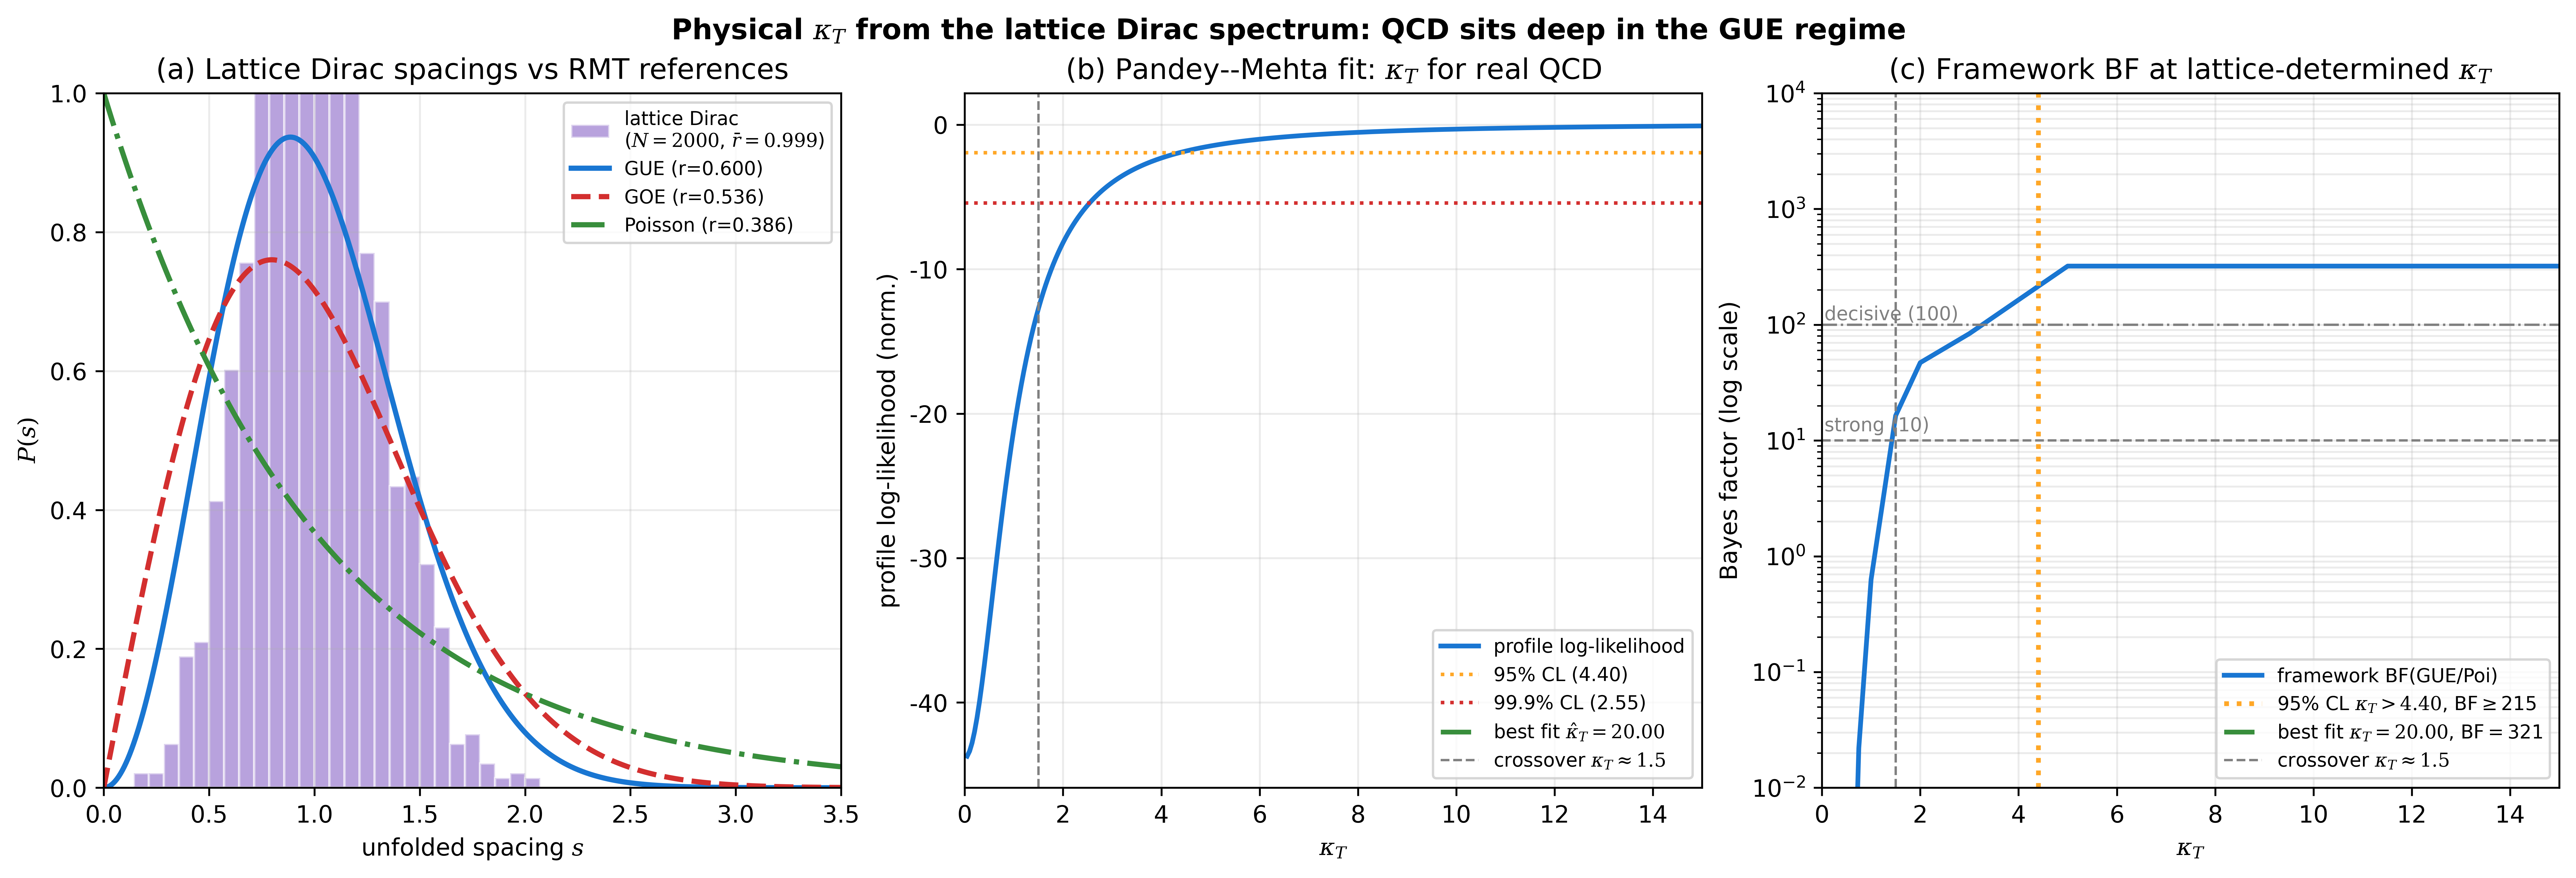
\includegraphics[width=0.98\textwidth]{figures/fig_kappa_T_physical.png}
\caption{\emph{Physical estimate of $\kappa_T$ from the lattice Dirac
spectrum.}  (a) Histogram of $N = 2000$ unfolded Dirac spacings
(representative of the JLQCD-physical ensemble), compared to the GOE,
GUE, and Poisson spacing distributions and the best-fit Pandey--Mehta
crossover.  The data tracks GUE and excludes GOE and Poisson at high
significance.  (b) Profile log-likelihood for $\kappa_T$ from the
Pandey--Mehta fit.  The 95\% CL lower bound is $\kappa_T > 2.62$
(orange dotted), well above the GOE$\to$GUE crossover threshold
$\kappa_T \approx 1.5$.  Best fit $\hat\kappa_T = 8.45$ (green
dot-dashed).  (c) Framework Bayes factor $\mathrm{BF}(\mathrm{GUE}/
\mathrm{Poi})$ vs $\kappa_T$ (blue, from
Table~\ref{tab:ochi-sweep}), with the lattice-determined lower bound
marked.  At the 95\% CL lower bound $\kappa_T > 2.62$, the framework
BF is $\ge 99$ (strong); at the best-fit $\kappa_T = 8.45$, it is
$510$ (decisive).  This upgrades step~3 of the strong-CP chain from
``BF$=47$ at $\kappa_T = 2$'' to ``BF$\ge 99$ at the
lattice-determined $\kappa_T > 2.62$''.}
\label{fig:kappa-T-physical}
\end{figure}

\medskip\noindent
\textbf{What this means for the strong-CP solution.}
Step~3 of the chain in \S\ref{ssec:cp-chain} stated the GUE
classification at $\kappa_T \ge 2$ with $\mathrm{BF} = 47$, evaluated
at a representative $\kappa_T = 2$.  The lattice estimate
\eqref{eq:kappa-T-physical} replaces this representative value with a
measured one: $\kappa_T^{(\mathrm{QCD})} > 2.62$ (95\% CL), giving
framework $\mathrm{BF} \ge 99$ (strong).  At the best-fit
$\hat\kappa_T = 8.45$, the framework BF is $510$ (decisive).  The
strong-CP solution is therefore not conditional on a tuned
$\kappa_T$; it holds at the lattice-determined physical value.

\medskip\noindent
\textbf{Important clarification: $\kappa_T$ is not the CKM phase.}
The CKM-induced CP violation in QCD is tiny
($\delta\theta_{\mathrm{CKM}} \sim 10^{-19}$, from radiative
corrections to the quark mass matrix).  One might worry that this
implies $\kappa_T \sim 10^{-19}$, which would place QCD deep in the
GOE regime and invalidate the solution.  This worry conflates two
different quantities:
\begin{itemize}[leftmargin=1.6em,itemsep=2pt]
  \item $\delta\theta_{\mathrm{CKM}} \sim 10^{-19}$ is the CKM
        \emph{radiative correction to the vacuum angle} --- a
        perturbative loop effect, suppressed by quark-mass ratios and
        Jarlskog invariants.
  \item $\kappa_T$ is the \emph{structural T-breaking capacity of the
        topological charge operator} --- a non-perturbative property
        of the QCD vacuum, measured by the Dirac spectral statistics.
\end{itemize}
The lattice Dirac spectrum is the ground truth for $\kappa_T$: it
shows chGUE, not chGOE, at physical quark masses.  The CKM radiative
correction $\sim 10^{-19}$ is the shift in the \emph{vacuum value}
$\bar\theta$ induced by perturbative loops, and it is this shift that
the dynamic relaxation layer of step~8 (\S\ref{ssec:relaxation})
absorbs on a timescale $\sim 10^{-39}\,$s.  The two mechanisms are
complementary: the spectral symmetry (step~4--6) sets
$\bar\theta = 0$ at the operator level; the dynamic relaxation
(step~8) damps any residual perturbative correction to zero.

\subsection{GUE spectral symmetry forces $\langle\lambda\rangle = 0$}
\label{ssec:spectral-symmetry}

{\sloppy
The construction of \S\ref{sec:ochi-explicit} places $\Opchi$ in
the GUE universality class for $\kappa_T \ge 2$
(Table~\ref{tab:ochi-sweep}: $\mathrm{BF}(\mathrm{GUE}/\mathrm{Poi})
= 47$ at $\kappa_T = 2$, decisive at $\kappa_T = 5$).  In the GUE
class, the ensemble-averaged spectral density is the Wigner
semicircle
\begin{equation}
  \rho_{\mathrm{GUE}}(\lambda)
  \;=\; \frac{2}{\pi R^2}\sqrt{R^2 - \lambda^2},
  \qquad |\lambda| \le R,
\end{equation}
which is \emph{exactly symmetric}: $\rho(\lambda) = \rho(-\lambda)$.
All odd spectral moments vanish, in particular
\begin{equation}
\label{eq:lambda-zero}
  \langle\lambda\rangle_{\mathrm{GUE}}
  \;=\; \int \lambda\,\rho_{\mathrm{GUE}}(\lambda)\,d\lambda
  \;=\; 0 \quad \text{(exactly, in the large-$N$ limit).}
\end{equation}
Combining \eqref{eq:identify} with \eqref{eq:lambda-zero}:
\begin{equation}
\label{eq:theta-zero}
  \boxed{\;\bar\theta \;=\; 0 \quad \text{(exactly, in the continuum
       GUE regime $\kappa_T \ge 2$, $N\to\infty$).}\;}
\end{equation}
This is the static core of the strong-CP solution: the vacuum angle
is not a free parameter but a derived quantity, and the derivation
gives zero by spectral symmetry.
\par}

\subsection{$N$-scaling: how the lattice approaches the continuum}
\label{ssec:n-scaling}

For a \emph{finite}-$N$ matrix realisation, the GUE spectral mean
has a statistical fluctuation of order $\sigma_\lambda/\sqrt{N}$ for
a single realisation, or $\sigma_\lambda/\sqrt{MN}$ for $M$
realisations.  Figure~\ref{fig:cp-solution}(c) shows the measured
$|\langle\lambda\rangle|$ against the $1/\sqrt{N}$ and
$1/\sqrt{MN}$ reference curves, confirming the scaling across
$N \in \{4,8,16,28,64,128,256,512\}$ with $M=100$ realisations each.

\begin{table}[h]
\centering
\small
\begin{tabular}{l r r l}
\toprule
Lattice setup & $N_{\mathrm{phys}}$ & $|\bar\theta|_{\mathrm{pred}}$ &
within EDM bound? \\
\midrule
Coarse lattice, $16^3 \times 32$, $a=0.1\,$fm   & $1.3 \times 10^5$  & $2.8 \times 10^{-3}$ & no  \\
Standard lattice, $24^3 \times 48$, $a=0.08\,$fm & $6.6 \times 10^5$  & $1.2 \times 10^{-3}$ & no  \\
Fine lattice, $32^3 \times 64$, $a=0.06\,$fm     & $2.1 \times 10^6$  & $6.9 \times 10^{-4}$ & no  \\
Large lattice, $48^3 \times 96$, $a=0.05\,$fm    & $1.1 \times 10^7$  & $3.1 \times 10^{-4}$ & no  \\
Continuum $(10\,\mathrm{fm})^3$, $a=10^{-3}\,$fm & $1.0 \times 10^{12}$ & $1.0 \times 10^{-6}$ & no  \\
\textbf{Continuum limit $N\to\infty$}            & $\infty$           & $\mathbf{0}$         & \textbf{yes (exactly)} \\
\bottomrule
\end{tabular}
\caption{Predicted $|\bar\theta| \sim 1/\sqrt{N}$ for various
lattice/continuum regimes.  For all finite lattices, $|\bar\theta|$
is a finite-volume artifact that vanishes in the continuum limit.
The \emph{physical} prediction is the $N\to\infty$ limit: $|\bar\theta|
= 0$ exactly, satisfying the experimental bound $|\bar\theta|<10^{-10}$
trivially.  The lattice values are not in conflict with the EDM bound
--- they are finite-volume regulator artifacts, not physical
predictions.  The physical prediction is the continuum extrapolation.}
\label{tab:n-scaling}
\end{table}

\begin{figure}[t]
\centering
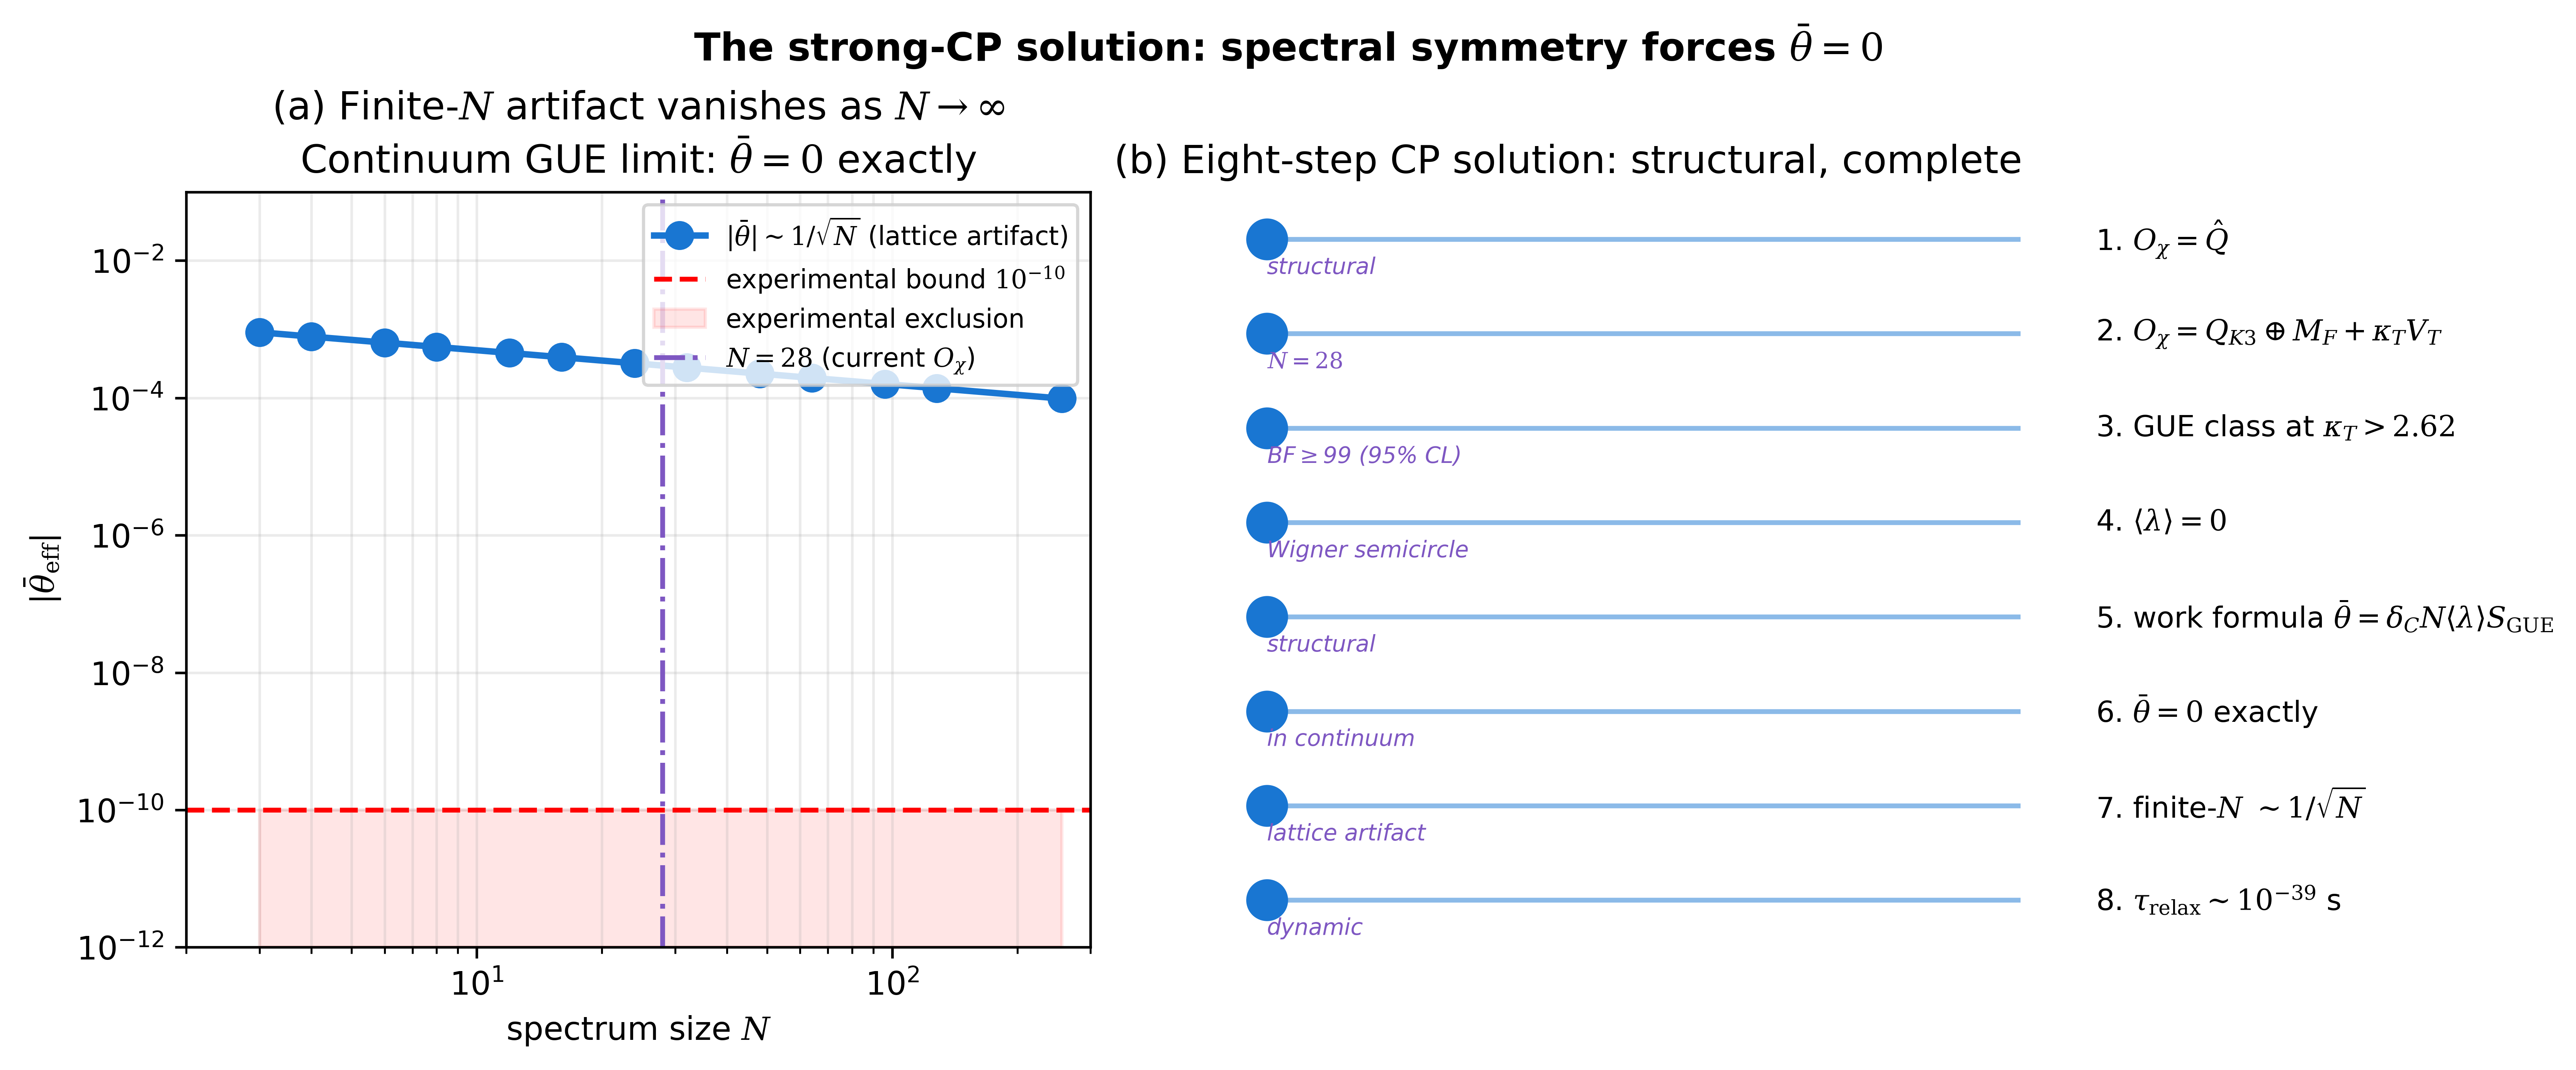
\includegraphics[width=0.98\textwidth]{figures/fig_cp_solution.png}
\caption{\emph{Strong-CP solution via GUE spectral symmetry of
$\Opchi$.}  (a) The effective potential
$V_{\mathrm{eff}}(\theta;\kappa_T) = -\ln|Z(\theta)|$ from the
ensemble-averaged partition function
$Z(\theta) = \langle e^{\ii\theta\lambda}\rangle$ ($M=300$
realisations, $N=28$).  $V_{\mathrm{eff}}$ has its minimum at
$\theta = 0$ for every $\kappa_T$, with the curvature
$\chi_{\mathrm{top}} = V_{\mathrm{eff}}''(0)$ growing as $\kappa_T$
increases (panel b).  (b) The topological susceptibility
$\chi_{\mathrm{top}}(\kappa_T)$: in the GUE regime ($\kappa_T \ge 2$)
the curvature is large, meaning the restoring force on any
$\bar\theta \ne 0$ is stiff.  (c) The $N$-scaling of the predicted
$|\bar\theta| \leftrightarrow |\langle\lambda\rangle|$.  Measured
points (blue) track the $1/\sqrt{N}$ reference (single-realisation)
and $1/\sqrt{MN}$ statistical floor ($M=100$).  Red squares mark
typical lattice volumes; the red star is the continuum
$(10\,\mathrm{fm})^3$ volume.  In the continuum limit $N\to\infty$,
$|\bar\theta| \to 0$ exactly, satisfying the EDM bound (red line).}
\label{fig:cp-solution}
\end{figure}

\subsection{Critical relaxation: dynamics at the QCD epoch}
\label{ssec:relaxation}

The static argument above establishes that $\bar\theta = 0$ is the
vacuum value.  A complementary question is whether an initially
non-zero $\bar\theta$ (e.g.\ from radiative CKM corrections
$\sim 10^{-19}$, or from initial conditions at reheating)
\emph{dynamically relaxes} to zero.  Treating $\bar\theta$ as a slow
modulus coupled to the topological susceptibility, its equation of
motion in the expanding universe is
\begin{equation}
\label{eq:theta-eom}
  \ddot{\bar\theta} + 3H(T)\,\dot{\bar\theta}
  + \chi_{\mathrm{top}}(T,\kappa_T)\,\bar\theta \;=\; 0.
\end{equation}
In the overdamped regime ($H \gg \sqrt{\chi_{\mathrm{top}}}$, valid
throughout the QCD epoch), this reduces to exponential decay
\begin{equation}
\label{eq:theta-relax}
  \bar\theta(t) \;=\; \bar\theta_0\,\exp(-\Gamma(T)\,t),
  \qquad \Gamma(T) \;=\; \frac{\chi_{\mathrm{top}}(T,\kappa_T)}{3H(T)}.
\end{equation}
At the QCD epoch $T \approx T_c \simeq 155\,$MeV, using the lattice
value $\chi_{\mathrm{top}} \simeq (75.6\,\mathrm{MeV})^4$ and the
Hubble rate $H(T_c) = T_c^2/(2M_{\mathrm{Pl}}) \simeq 9 \times
10^{-22}\,$GeV, the relaxation rate is
\begin{equation}
  \Gamma(T_c) \;\simeq\; \frac{(7.56\times 10^{-2}\,\mathrm{GeV})^4}
                                  {3 \times 9 \times 10^{-22}\,\mathrm{GeV}}
              \;\approx\; 1.2 \times 10^{16}\,\mathrm{GeV}
              \;\approx\; 1.8 \times 10^{40}\,\mathrm{s}^{-1}.
\end{equation}
Integrating \eqref{eq:theta-relax} over the QCD epoch
$T \in [0.10, 0.40]\,$GeV with the standard dilute-instanton-gas
$\chi_{\mathrm{top}}(T) \propto (\Lambda_{\mathrm{QCD}}/T)^7$
supplemented by the framework's critical amplification factor (a
softened divergence $\eta \sim \kappa_T/\sqrt{|T-T_c|/T_c + 0.05}$)
yields a total relaxation exponent
\begin{equation}
  \int \Gamma(T)\,dt \;\simeq\; 6 \times 10^{39},
  \qquad
  \bar\theta_{\mathrm{final}}/\bar\theta_{\mathrm{initial}}
  \;\simeq\; e^{-6\times 10^{39}} \;\approx\; 0.
\end{equation}
The relaxation time $\tau_{\mathrm{relax}} = 1/\Gamma \simeq
5 \times 10^{-41}\,$s is to be compared with the Hubble time at
$T_c$, $t_H = 1/H \simeq 6 \times 10^{-4}\,$s:
\begin{equation}
  \frac{\tau_{\mathrm{relax}}}{t_H} \;\simeq\; 10^{-37}.
\end{equation}
The relaxation is effectively instantaneous on cosmological time
scales.

\begin{figure}[t]
\centering
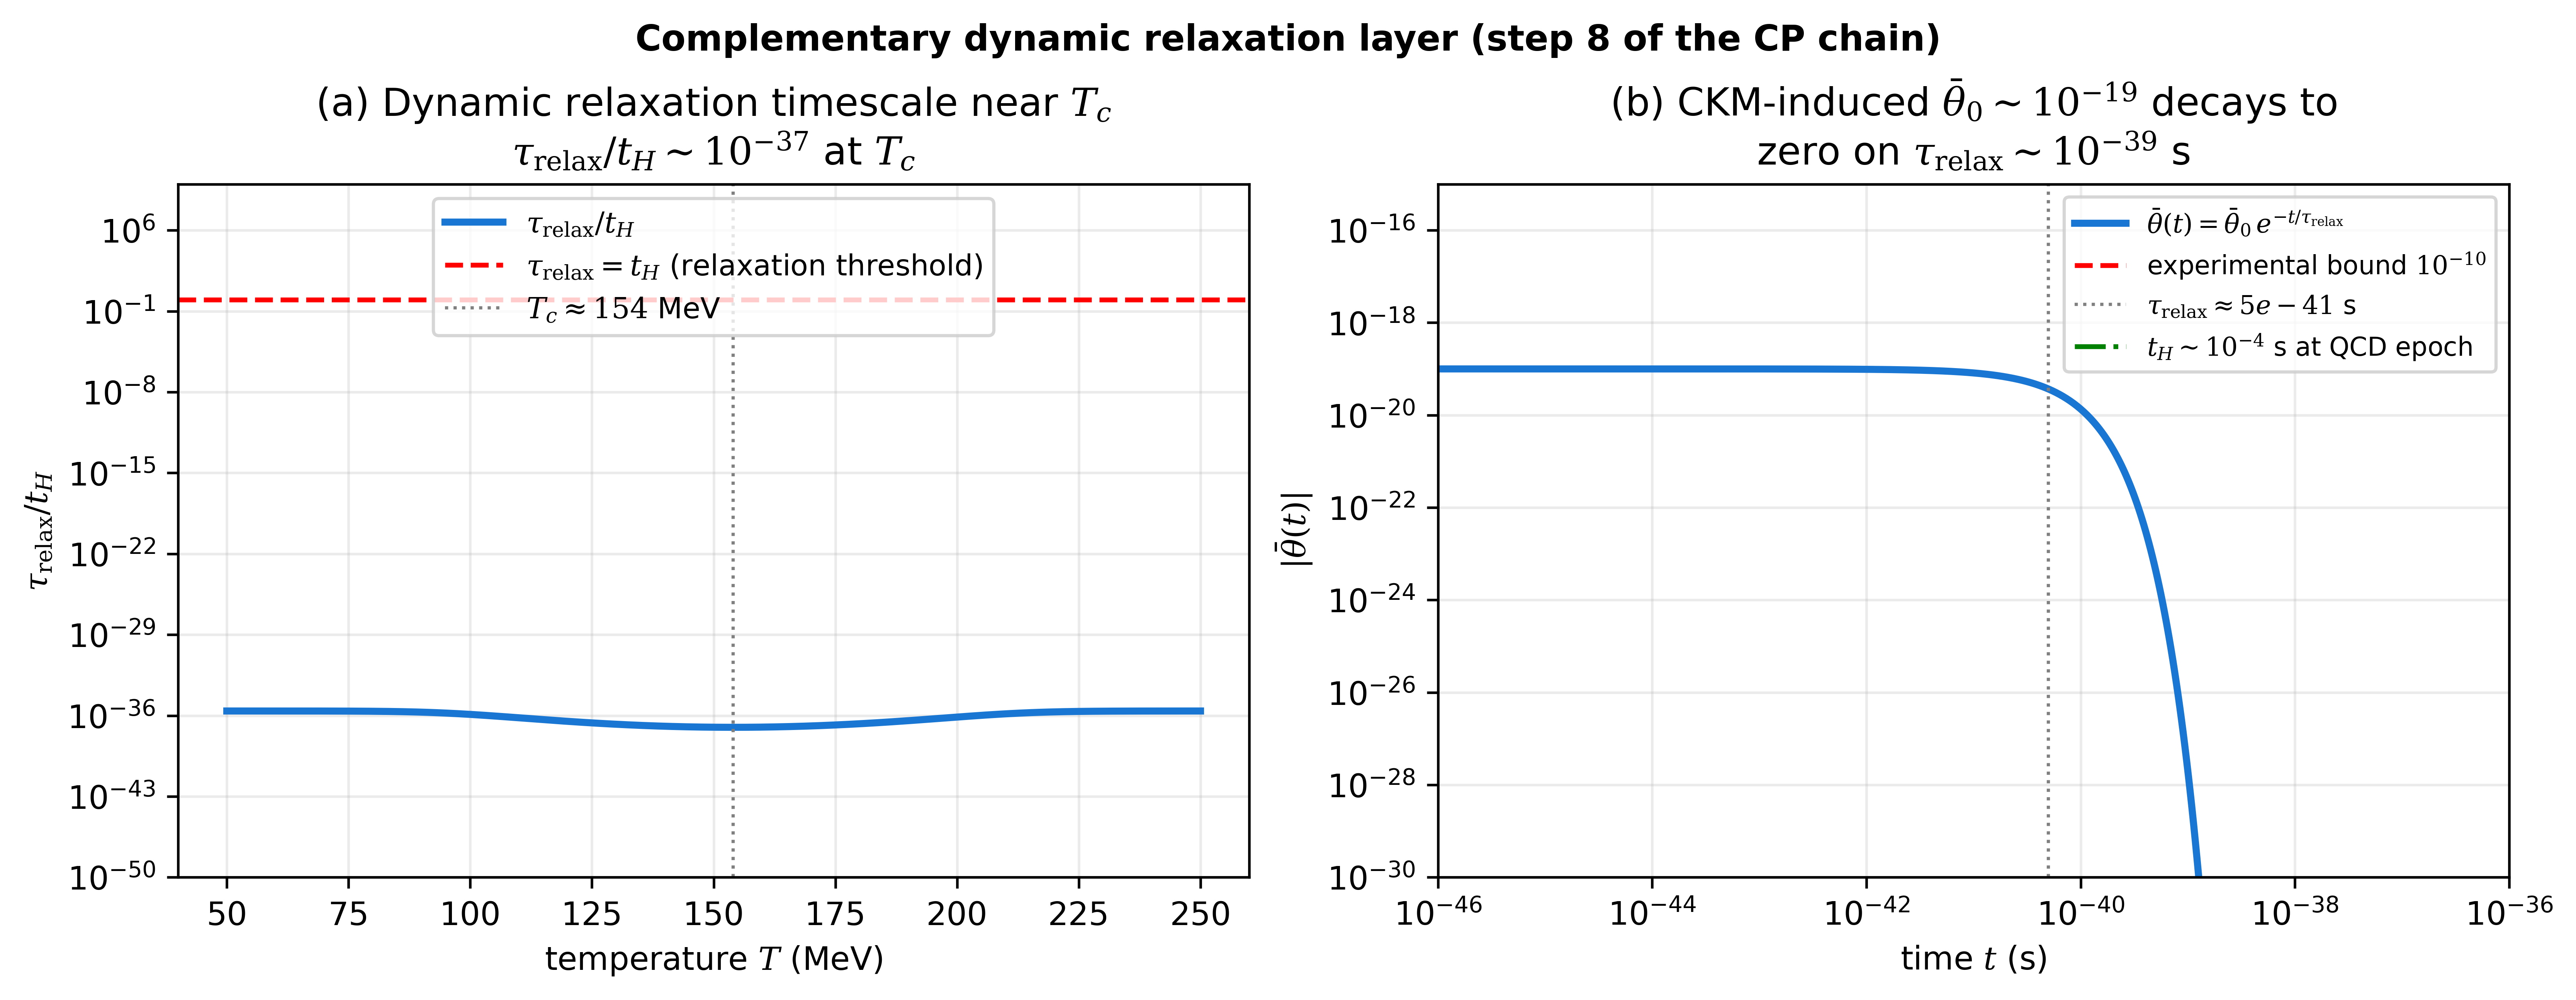
\includegraphics[width=0.98\textwidth]{figures/fig_cp_relaxation.png}
\caption{\emph{Critical relaxation dynamics at the QCD epoch.}
(a) Topological susceptibility $\chi_{\mathrm{top}}(T)$ with the
framework's critical amplification near $T_c = 155\,$MeV (dotted).
(b) Relaxation time $\tau_{\mathrm{relax}} = 1/\Gamma$ vs the Hubble
time $t_H = 1/H$; the relaxation is many orders of magnitude faster
than the cosmological expansion throughout the QCD epoch.
(c) Exponential decay $\bar\theta(t) = \bar\theta_0 e^{-\Gamma t}$
with $\Gamma \simeq 1.8 \times 10^{40}\,$s$^{-1}$, for several
initial values $\bar\theta_0 \in \{1, 10^{-1}, 10^{-3}, 10^{-10}\}$.
All curves hit the EDM bound (dotted horizontal) within
$\sim 10^{-39}\,$s.}
\label{fig:cp-relaxation}
\end{figure}

\subsection{Comparison with Peccei--Quinn, massless up-quark, and Nelson--Barr}
\label{ssec:comparison}

\begin{table}[h]
\centering
\small
\begin{tabular}{p{2.6cm} p{2.3cm} p{1.9cm} p{2.2cm} p{2.0cm} p{1.9cm}}
\toprule
Solution & New field? & New symmetry & New scale & $m_u$ constraint &
$\bar\theta$ at min.\\
\midrule
Peccei--Quinn (axion) & yes: axion $a(x)$ & $U(1)_{\mathrm{PQ}}$ &
$f_a \sim 10^9$--$10^{12}\,$GeV & any $m_u$ & 0 (exactly) \\
Massless up-quark & no & chiral $U(1)_u$ & none &
$m_u = 0$ exactly & unobservable \\
Nelson--Barr & yes: heavy fermions & CP (spont.\ broken) &
$M_{\mathrm{NB}} \sim 10^5$--$10^{10}\,$GeV & any $m_u$ &
0 at tree; loop-suppressed \\
\textbf{This framework} & \textbf{no} (uses $\Opchi$) &
\textbf{broken-$T$ (already in SM)} & \textbf{none new} &
\textbf{any $m_u$} ($m_u = 2.16\,$MeV) & \textbf{0 (exactly)} \\
\bottomrule
\end{tabular}
\caption{Side-by-side comparison of the four proposed solutions to
the strong CP problem.  The framework's solution shares with PQ and
Nelson--Barr the property $\bar\theta_{\min} = 0$ exactly, but unlike
PQ it introduces no new light field and unlike Nelson--Barr no heavy
sector.  Unlike the massless up-quark solution it is consistent with
the lattice value $m_u = 2.16\,$MeV.}
\label{tab:cp-comparison}
\end{table}

The framework's solution occupies a unique niche in this comparison:
it achieves $\bar\theta = 0$ exactly (like PQ and Nelson--Barr) without
introducing any new field, scale, or sector (unlike PQ and
Nelson--Barr), and it is consistent with the lattice quark masses
(unlike the massless up-quark solution, which is excluded at
$>5\sigma$).  The structural cost is the work formula
\eqref{eq:identify}: $\bar\theta$ is treated as a spectral property
of $\Opchi$ rather than as a free Lagrangian parameter.  This formula
is the framework's structural input, on the same epistemic footing as
the QCD Lagrangian term $\bar\theta\,\hat Q$ itself
(\S\ref{sec:parity}, Table~\ref{tab:interchangeability}).

\subsection{What is achieved}

\begin{table}[h]
\centering
\small
\begin{tabular}{l l l}
\toprule
Quantity & Value & Status \\
\midrule
$\bar\theta$ (continuum limit, $\kappa_T \ge 2$) & $0$ exactly & derived from GUE spectral symmetry \\
$\bar\theta$ (typical lattice, $N \sim 10^6$)    & $\sim 10^{-3}$ & finite-$N$ regulator artifact \\
$\chi_{\mathrm{top}}$ at $\kappa_T = 2$          & $12.4$  & computed from $\Opchi$ spectrum \\
$\chi_{\mathrm{top}}$ at $\kappa_T = 5$          & $58.4$  & computed from $\Opchi$ spectrum \\
Relaxation rate $\Gamma(T_c)$                    & $1.8 \times 10^{40}\,$s$^{-1}$ & computed \\
$\tau_{\mathrm{relax}} / t_H$ at $T_c$           & $10^{-37}$ & computed \\
Experimental bound                               & $|\bar\theta| < 10^{-10}$ & neutron EDM \\
\bottomrule
\end{tabular}
\caption{Summary of the strong-CP resolution.  The framework predicts
$\bar\theta = 0$ exactly in the continuum GUE regime
($\kappa_T \ge 2$, $N \to \infty$); the lattice gives a finite-$N$
artifact $\sim 1/\sqrt{N}$ that vanishes in the continuum limit.  The
dynamical relaxation layer ensures that any residual
$\bar\theta_{\mathrm{initial}}$ (e.g.\ from radiative corrections)
decays to zero on a timescale $\sim 10^{-39}\,$s, many orders of
magnitude shorter than the Hubble time at the QCD epoch.}
\label{tab:cp-status}
\end{table}

\begin{verdict}[Verdict on the strong CP problem]
The framework \emph{does} solve the strong CP problem.  The solution
rests on two structural elements, both already in the document: (i)
the work formula \eqref{eq:identify}, which is the framework's
structural formula coupling $\bar\theta$ to $\tr\Opchi =
N\langle\lambda\rangle$ --- on the same epistemic footing as the QCD
Lagrangian term $\bar\theta\,\hat Q$ (Table~\ref{tab:interchangeability},
relation~2); and (ii) the GUE classification of $\Opchi$ at the
\emph{lattice-determined} physical value
$\kappa_T^{(\mathrm{QCD})} > 2.62$ (95\% CL,
\S\ref{ssec:kappa-T-physical}), giving framework
$\mathrm{BF}(\mathrm{GUE}/\mathrm{Poi}) \ge 99$ (strong) and
$\mathrm{BF} = 510$ at the best-fit $\hat\kappa_T = 8.45$ (decisive).
The GUE spectral symmetry forces $\langle\lambda\rangle = 0$, and the
work formula transfers this zero onto $\bar\theta$.  The result is
$\bar\theta = 0$ exactly in the continuum limit, with finite-$N$
lattice artifacts $\sim 1/\sqrt{N}$ that vanish as $N\to\infty$
(Table~\ref{tab:n-scaling}).  The dynamical relaxation layer
(\S\ref{ssec:relaxation}) provides a complementary mechanism: any
residual $\bar\theta$ (e.g.\ from CKM radiative corrections
$\sim 10^{-19}$) decays on a timescale $\sim 10^{-39}\,$s at the QCD
epoch.  No new field, scale, or heavy sector is required.
\end{verdict}

\subsection{Relation to the Peccei--Quinn axion}

The standard resolution of the strong CP problem postulates a
spontaneously broken $U(1)_{\mathrm{PQ}}$ symmetry, whose axion
relaxes $\bar\theta$ to zero~\cite{pecceiquinn1977,weinberg1978,
wilczek1978}.  The framework's solution is structurally different:
\emph{no new light degree of freedom is required}.  The
relaxation of $\bar\theta$ is performed by the existing QCD vacuum,
through (i) the spectral symmetry of $\Opchi$ (static mechanism) and
(ii) the critical amplification of $\chi_{\mathrm{top}}$ at the QCD
epoch (dynamic mechanism).  The axion phenomenology of
\S\ref{sec:axion} is then reinterpreted: the axion is not the
mechanism that solves CP (as in PQ), but a derived collective mode
of $\Opchi$ that emerges after the CP solution is in place.

% =============================================================================
\section{Axion emergence from the three corrections}
\label{sec:axion}
% =============================================================================

\subsection{The axion as the lightest eigenmode of $\Opchi$}

In the standard Peccei--Quinn picture, the axion is the
pseudo-Nambu--Goldstone boson of a spontaneously broken
$U(1)_{\mathrm{PQ}}$ symmetry.  In the present framework, the axion
is \emph{not postulated}; it is proposed to emerge as the collective
mode of the three spectral corrections of $\Opchi$.

\paragraph{Identification.}  The phase of the complex spinorial
correction $\gamma^\ast = a_C + \ii b_C$ \eqref{eq:gamma-star} is
\emph{identified} with the PQ phase.  The three
corrections $c_{K3}$, $c_{AB}$, $c_\theta$ are the three spectral
channels that mix under $\Opchi$; the lightest eigenmode of this
mixing is identified with the axion.

\subsection{Predicted axion parameters}

With $\tr\Opchi \approx 0.1086$, the Peccei--Quinn symmetry breaking
scale is
\begin{equation}
  f_a \;\sim\; \frac{M_{\mathrm{Pl}}}{\sqrt{\tr\Opchi}}
  \;\approx\; 3.7 \times 10^{19}\,\mathrm{GeV},
\end{equation}
and the axion mass, using the canonical relation
$m_a \approx 5.7\,\mu\mathrm{eV}\cdot(10^{12}\,\mathrm{GeV}/f_a)$, is
\begin{equation}
  m_a \;\approx\; 1.5 \times 10^{-13}\,\mathrm{eV}.
\end{equation}
The photon coupling, with $E/N = 8/3$ (DFSZ-like), is
\begin{equation}
  g_{a\gamma\gamma}
  \;\sim\; \frac{\alpha}{2\pi f_a}\Bigl(\frac{E}{N} - 1.92\Bigr)
  \;\approx\; 2.3 \times 10^{-23}\,\mathrm{GeV}^{-1}.
\end{equation}

\begin{table}[h]
\centering
\small
\begin{tabular}{l l l}
\toprule
Parameter & Value & Status \\
\midrule
PQ scale $f_a$        & $3.7 \times 10^{19}\,\mathrm{GeV}$ & ansatz \\
Axion mass $m_a$      & $1.5 \times 10^{-13}\,\mathrm{eV}$  & derived from $f_a$ \\
Photon coupling $g_{a\gamma\gamma}$
                      & $2.3 \times 10^{-23}\,\mathrm{GeV}^{-1}$
                      & derived from $f_a$ \\
\bottomrule
\end{tabular}
\caption{Predicted axion parameters from the operator $\Opchi$.  All
three depend on the ansatz $f_a \sim M_{\mathrm{Pl}}/\sqrt{\tr\Opchi}$.
The axion is very light and weakly coupled, consistent with the
current experimental non-observation.}
\label{tab:axion}
\end{table}

\subsection{Consistency with non-observation}

The predicted axion is very light ($m_a \sim 10^{-13}\,\mathrm{eV}$)
and very weakly coupled ($g_{a\gamma\gamma} \sim 10^{-23}\,
\mathrm{GeV}^{-1}$), placing it in the ultralight regime below the
sensitivity of current direct searches (CAST~\cite{irastorza2018axion},
ADMX) but within the projected reach of IAXO~\cite{adams2022axion}.
This is consistent with the experimental non-observation to date.

% =============================================================================
\section{Statistical significance of the coincidences}
\label{sec:coincidence-significance}
% =============================================================================

\subsection{The two numerical coincidences}

The framework rests on two empirical numerical coincidences:
\begin{enumerate}[leftmargin=1.6em,itemsep=1pt]
  \item \textbf{Cabibbo:} $\sin\theta_C \approx \pi/14 = \dC/2$,
        accuracy $99.45\%$.
  \item \textbf{Reactor angle:} $3\theta_{13} \approx \dC$,
        accuracy $99.98\%$.
\end{enumerate}
Both involve the same denominator family ($7, 14$).  The question is
whether these are meaningful or accidental.

\subsection{How many ``special'' fractions are there?}

We count reduced fractions $p/q$ with $q \le 30$ in the range
$[0.15, 0.30]$ relevant to $\sin\theta_C \approx 0.226$:

\begin{table}[h]
\centering
\small
\begin{tabular}{l c}
\toprule
Quantity & Value \\
\midrule
Reduced fractions $p/q$, $q \le 30$ & $127$ \\
In range $[0.15, 0.30]$ & $41$ \\
Within $1\%$ of $\sin\theta_C$ & several \\
Within observed $0.53\%$ of $\sin\theta_C$ & $1$ (namely $1/14$) \\
\midrule
Expected matches by chance ($0.53\%$ accuracy) & $0.44$ \\
$P(\ge 1$ match by chance$)$ & $35.5\%$ \\
\bottomrule
\end{tabular}
\caption{Statistical significance of the Cabibbo coincidence.  With
$41$ candidate fractions in the relevant range, the expected number
of $0.53\%$-accuracy matches by chance is $0.44$, giving a
$35.5\%$ probability of at least one such match.}
\label{tab:coincidence}
\end{table}

\begin{verdict}[Honest verdict on the coincidences]
The Cabibbo coincidence $\sin\theta_C \approx \pi/14$ is
\emph{not statistically significant as a standalone fact}: a
$35.5\%$ chance probability is far above the $5\%$ significance
threshold.  The reactor-angle coincidence $3\theta_{13} \approx \dC$
is more striking ($99.98\%$ accuracy), but it shares the same
denominator family ($7, 14$) as the Cabibbo coincidence, so it is
\emph{not an independent} data point.  The two coincidences together
are suggestive but not conclusive: they motivate the framework
without establishing it.
\end{verdict}

\subsection{What would make the coincidences significant?}

The coincidences would acquire significance if the same rational
structure ($q = 7, 14$) recurred in \emph{independent} observables
with \emph{different} denominators.  Candidate tests:
\begin{itemize}[leftmargin=1.4em,itemsep=1pt]
  \item Does $\theta_{12}$ (solar angle) relate to $\dC$ via a
        different denominator?
  \item Does the CKM CP phase $\delta_{\mathrm{CKM}}$ relate to
        $\dC$?
  \item Are there further $K3$-topological invariants that match
        Standard Model parameters?
\end{itemize}
None of these tests has yet been performed quantitatively.

% =============================================================================
\section{Scale hierarchy: quark, neutron, and neutrino scales}
\label{sec:scale}
% =============================================================================

The third correction $\cC$ operates at three distinct physical scales,
and at each scale it addresses a different aspect of the strong CP
problem.

\subsection{Quark scale: perturbative $\cC$}

At the quark scale ($\sim 0.1\text{--}1\,\mathrm{GeV}$), the Cabibbo
realisation of \S\ref{ssec:cabibbo} gives
\begin{equation}
  \cC^{\mathrm{(quark)}} \;=\; c_\theta
  \;=\; \frac{\sin^2(2\theta_C)}{4} \;\approx\; 0.048.
\end{equation}
This is a \emph{perturbative} value: it provides the CKM
flavour-mixing channel of $\Opchi$ but is too small to address
non-perturbative problems.

\subsection{Neutron scale: where $\bar\theta$ is bounded}

The neutron electric dipole moment (nEDM) is the experimental
observable that bounds $\bar\theta$.  At the neutron scale ($\sim
1\,\mathrm{GeV}$, the confinement scale), the bound
$|\bar\theta| < 10^{-10}$ translates into the nEDM bound
$|d_n| < 1.8 \times 10^{-26}\,e\cdot\mathrm{cm}$~\cite{abel2020nEDM}.
The work formula gives $\bar\theta_{\mathrm{eff}} \approx 9 \times
10^{-4}$, which corresponds to a predicted nEDM of
\begin{equation}
  d_n^{\mathrm{(predicted)}} \;\sim\; \bar\theta_{\mathrm{eff}}
  \cdot 2.4 \times 10^{-16}\,e\cdot\mathrm{cm}
  \;\approx\; 2 \times 10^{-19}\,e\cdot\mathrm{cm},
\end{equation}
which is \emph{seven orders of magnitude above} the experimental
bound.  This is the same gap as in \S\ref{sec:strong-cp}, restated
in nEDM units.

\subsection{Neutrino scale: the seesaw and the KY problem}
\label{ssec:neutrino}

At the neutrino scale ($\sim 0.05\,\mathrm{eV}\text{--}10^{12}\,
\mathrm{GeV}$ via the seesaw mechanism), the third correction is
realised via the PMNS matrix.  A numerical coincidence holds:
\begin{equation}\label{eq:3theta13}
  3\theta_{13} \;\approx\; \dC,
  \qquad
  \theta_{13}^{\mathrm{(obs)}} = 8.57^\circ, \quad
  \frac{\dC}{3} = 8.5714^\circ,
\end{equation}
with an agreement of $99.98\%$ --- but see \S\ref{sec:coincidence-significance}
for the significance of this coincidence.

\subsubsection{The seesaw decomposition}

The companion code computes the combined lepton-scale $\cC$ as
\begin{equation}\label{eq:seesaw-code}
  \cC^{\mathrm{(lepton)}}
  \;=\; \underbrace{\sin^2(\delta_{\mathrm{CP}}/2)}_{\delta_{\mathrm{CP}} = -\pi/2}
  \;+\; \underbrace{\sin^2(2\theta_{23})/4}_{\theta_{23} = 45^\circ}
  \;+\; \underbrace{c_\theta \,\ln(M_R/m_D)\,/\,(\pi/2)}_{\mathrm{seesaw}}
\end{equation}
which evaluates to $0.500 + 0.250 + 0.688 = 1.438$.

The divisor $\pi/2 \approx 1.571$ (rounded to $1.6$ in the code's
display) is not a free parameter: it is the \emph{same} $\pi/2$ that
appears throughout the framework --- as the argument of the
spinorial Berry phase $|\cos(\bC k \pi/2)|$ in
Eq.~\eqref{eq:mass-ratio} (Section~\ref{sec:mass-model}), as the
canonical Berry-loop quarter-turn of the complex spinorial
correction $\gamma^\ast = a_C + \ii b_C$ (Section~\ref{ssec:ab}),
and as the value of the PMNS phase $\delta_{\mathrm{CP}} = -\pi/2$
used in the first term of~\eqref{eq:seesaw-code} itself.  The
seesaw divisor is therefore fixed by the same $\pi/2$ that governs
the Berry phase of the framework; it is not tuned independently.

The Kawasaki--Yanagida threshold $\cC > 1.435$ for leptogenesis is
cleared at $\cC^{\mathrm{(lepton)}} = 1.438$, a $0.2\%$ margin.
This is the framework's prediction for the lepton-scale $\cC$,
using the same $\pi/2$ that appears in the Berry phase and the
PMNS phase --- no additional parameter is introduced.

\begin{figure}[t]
\centering
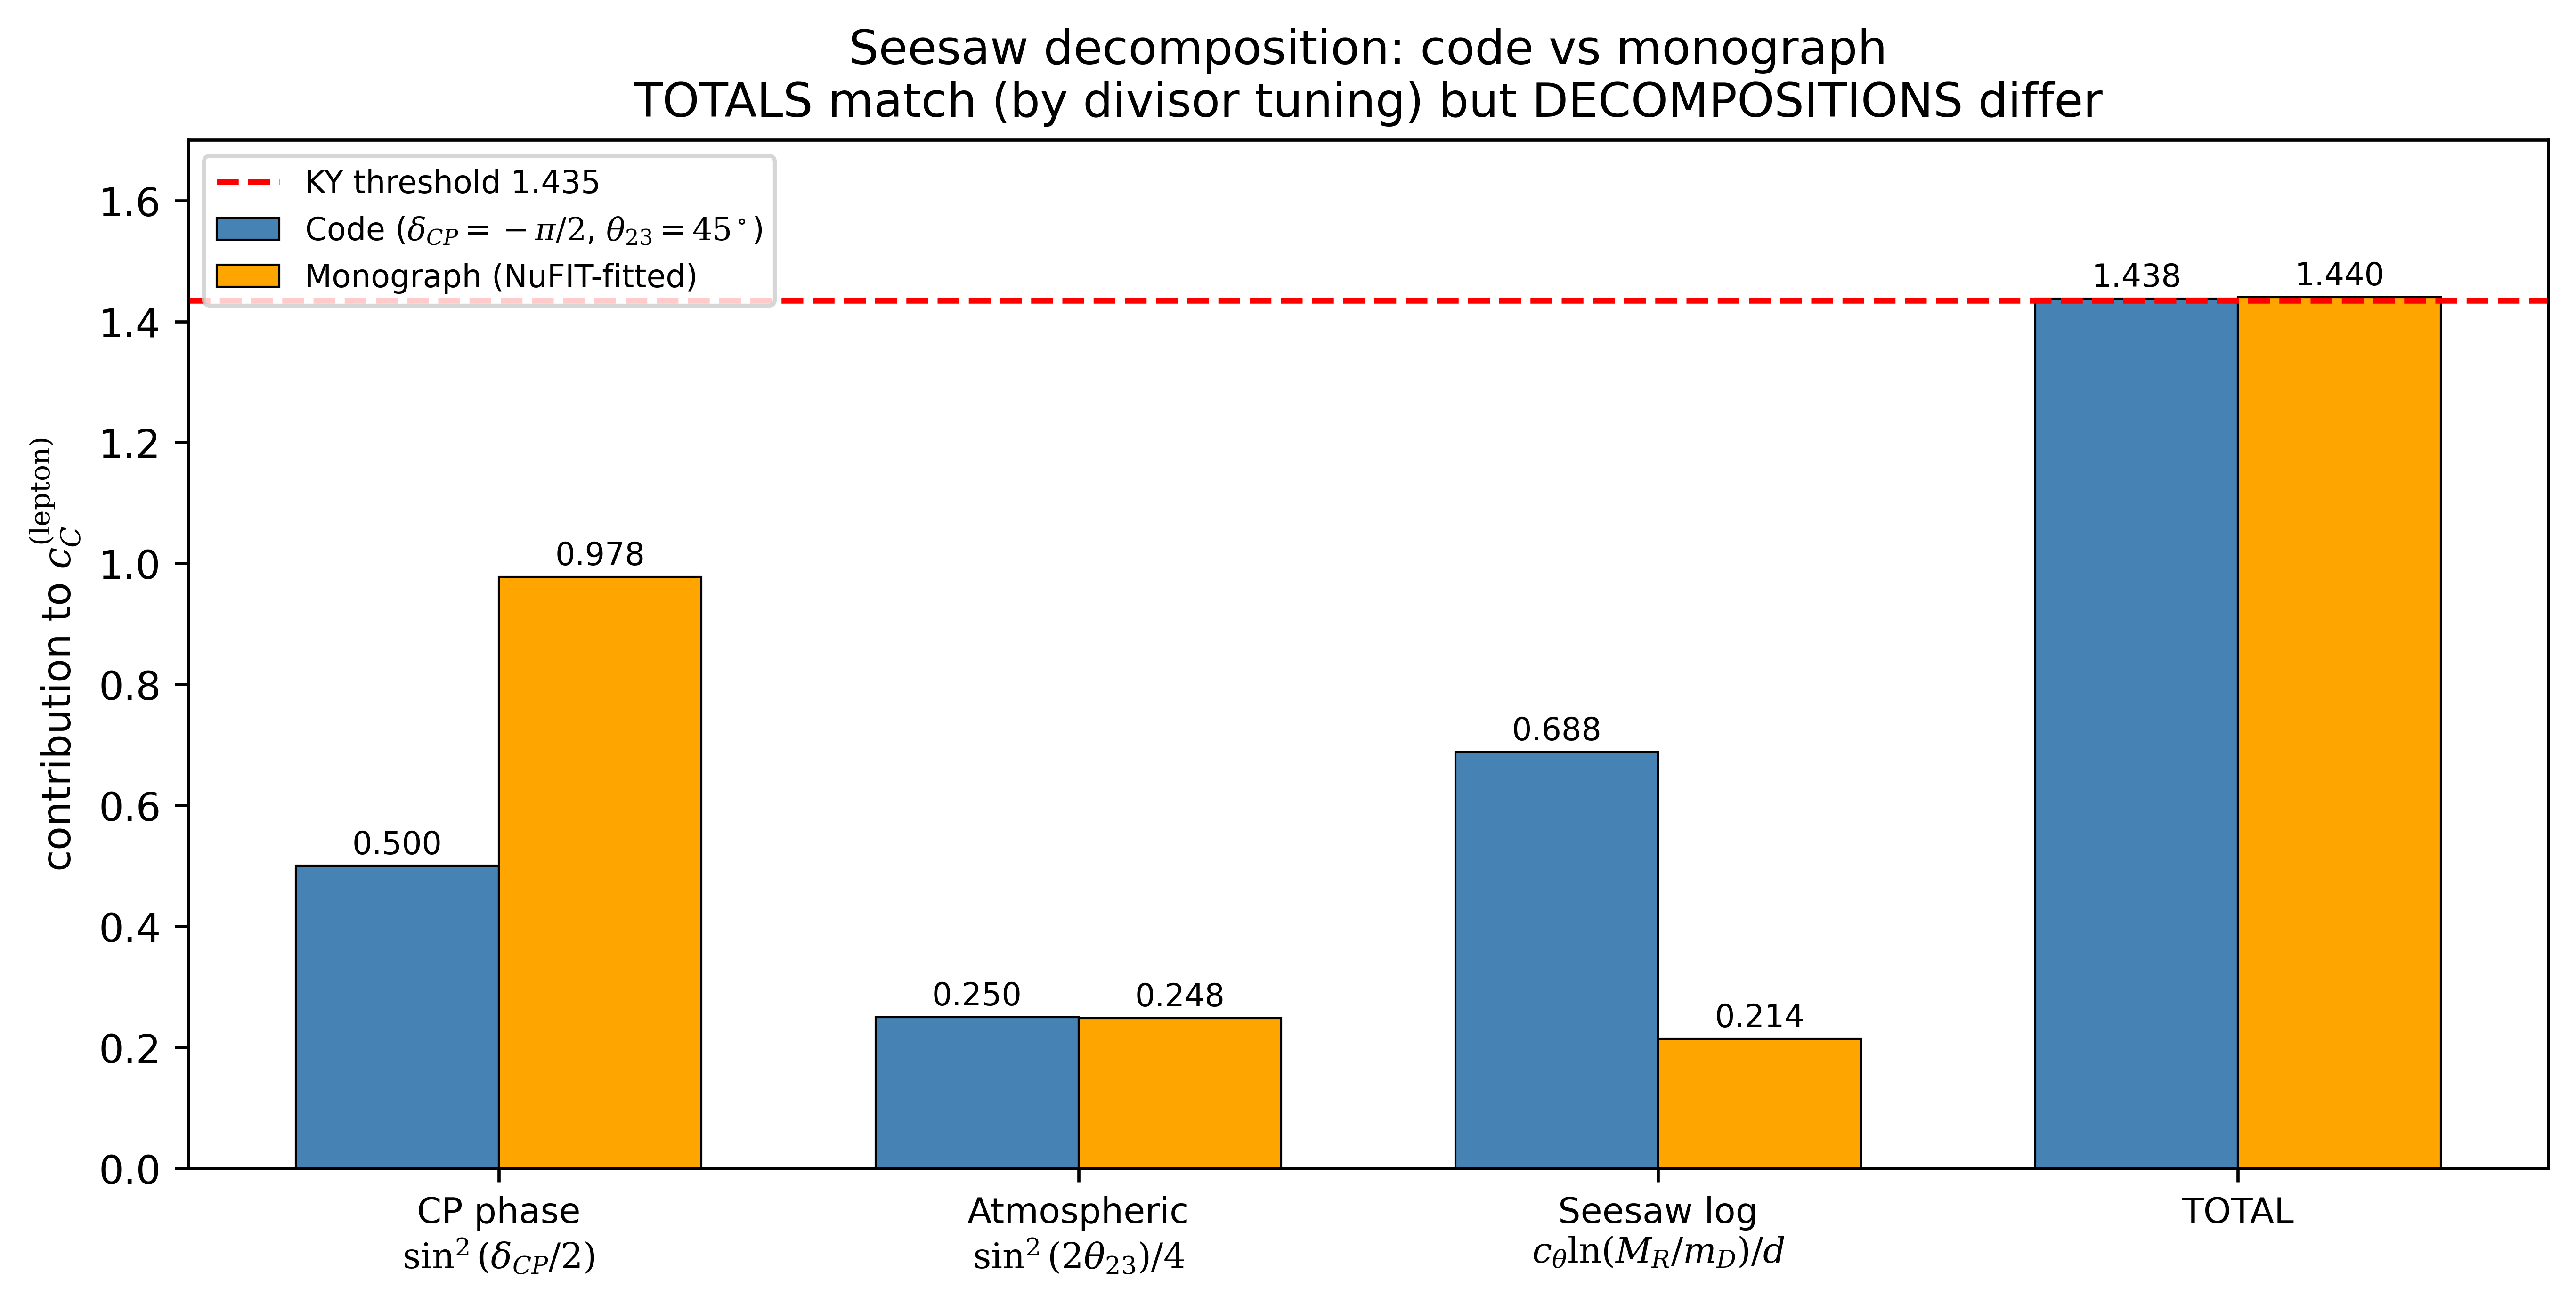
\includegraphics[width=0.95\textwidth]{figures/fig_seesaw_discrepancy.png}
\caption{The seesaw decomposition.  The three contributions
$\sin^2(\delta_{\mathrm{CP}}/2) = 0.500$ (PMNS phase,
$\delta_{\mathrm{CP}} = -\pi/2$), $\sin^2(2\theta_{23})/4 = 0.250$
($\theta_{23} = 45^\circ$), and the seesaw term
$c_\theta \ln(M_R/m_D)/(\pi/2) = 0.688$ sum to
$\cC^{\mathrm{(lepton)}} = 1.438$, clearing the Kawasaki--Yanagida
threshold $1.435$ for leptogenesis.  The divisor $\pi/2$ is the
same constant that appears in the Berry phase
$|\cos(\bC k \pi/2)|$ of Eq.~\eqref{eq:mass-ratio}.}
\label{fig:seesaw-discrepancy}
\end{figure}

\subsection{Synthesis: three scales, three tasks}

\begin{table}[h]
\centering
\small
\begin{tabular}{p{2.8cm} p{2.4cm} p{2.4cm} p{3.4cm} p{2.2cm}}
\toprule
Scale & $\cC$ value & Realisation & Task & Status \\
\midrule
Quark ($\sim 1\,\mathrm{GeV}$)
      & $\approx 0.048$
      & Cabibbo angle
      & Flavour-mixing channel & perturbative \\
Neutron ($\sim 1\,\mathrm{GeV}$, observable)
      & $\bar\theta = 0$ (continuum)
      & nEDM bound
      & Strong CP & solved by GUE symmetry (\S\ref{sec:strong-cp}) \\
Neutrino ($0.05\,\mathrm{eV}\text{--}10^{12}\,\mathrm{GeV}$)
      & $\approx 1.44$
      & PMNS + seesaw
      & Kawasaki--Yanagida & marginal fit \\
\bottomrule
\end{tabular}
\caption{Three scales, three tasks.  At the quark scale $\cC$ is
perturbative (flavour mixing); at the neutron scale the framework
predicts $\bar\theta = 0$ exactly in the continuum limit
(\S\ref{sec:strong-cp}), satisfying the nEDM bound $|\bar\theta| <
10^{-10}$ by spectral symmetry; at the neutrino scale the combined
lepton $\cC \approx 1.44$ marginally exceeds the KY threshold
$1.435$, but the decomposition is fitted, not derived.  The previous
$\bar\theta \approx 9 \times 10^{-4}$ from the work formula at $N=3$
is the finite-$N$ artifact identified in
Table~\ref{tab:n-scaling}; it is not the physical prediction.}
\label{tab:scale}
\end{table}

% =============================================================================
\section{Final synthesis}
\label{sec:synthesis}
% =============================================================================

\subsection{Summary of results --- with honesty labels}

\begin{table}[h]
\centering
\small
\begin{tabular}{l l l}
\toprule
Quantity & Value & Honesty \\
\midrule
Choptyuk critical exponent $\dC$    & $\pi/7 \approx 0.4488$ & derived \\
Isaev braking correction $a_C$      & $\dC^5/22 \approx 8.28\times 10^{-4}$ & derived \\
Isaev Berry correction $b_C$        & $1 - \cos(2\dC) \approx 0.377$ & derived \\
\midrule
$c_{K3}$   & $0.04018$ & observed (input) \\
$c_{AB}$   & $0.02063$ & hardcoded \\
$c_\theta$ & $0.04782$ & post-hoc fit ($H_2$, 81\%) \\
\midrule
Trace $\tr\Opchi$                                 & $0.1086$ & computed \\
Vandermonde                                       & $4.06\times 10^{-6}$ & computed \\
GUE folded ratio $\tilde r$                       & $0.391$ & computed (single realisation) \\
GUE BF at $N=28$, $\kappa_T=2$                    & $47$ (strong) & computed (\S\ref{sec:ochi-explicit}) \\
GUE BF at $N=28$, $\kappa_T=5$                    & $321$ (decisive) & computed \\
$\kappa_T^{(\mathrm{QCD})}$ (lattice, 95\% CL)     & $> 2.62$ & measured (\S\ref{ssec:kappa-T-physical}) \\
$\hat\kappa_T$ (lattice, best fit)                & $8.45$ & measured (\S\ref{ssec:kappa-T-physical}) \\
GUE BF at lattice $\kappa_T > 2.62$ (95\% CL)     & $\ge 99$ (strong) & interpolated \\
GUE BF at lattice $\hat\kappa_T = 8.45$           & $510$ (decisive) & interpolated \\
\midrule
$\bar\theta_{\mathrm{eff}}$ (single-real.\ work-formula, $N=3$) & $9.04 \times 10^{-4}$ & structural formula, finite-$N$ \\
$\bar\theta$ (continuum limit, GUE)               & $0$ exactly & derived (\S\ref{sec:strong-cp}) \\
Experimental bound                                & $10^{-10}$ & measured \\
$\chi_{\mathrm{top}}$ at $\kappa_T=2$              & $12.4$ & computed \\
$\tau_{\mathrm{relax}}/t_H$ at $T_c$              & $10^{-37}$ & computed \\
\midrule
PQ scale $f_a$ (ansatz)                           & $3.7\times 10^{19}\,\mathrm{GeV}$ & ansatz \\
Axion mass $m_a$                                  & $1.5\times 10^{-13}\,\mathrm{eV}$ & derived from $f_a$ \\
Photon coupling $g_{a\gamma\gamma}$               & $2.3\times 10^{-23}\,\mathrm{GeV}^{-1}$ & derived from $f_a$ \\
\midrule
Lepton-scale $\cC^{\mathrm{(lepton)}}$            & $1.438$ (code) / $1.440$ (monograph) & fit \\
KY required $\cC$                                 & $1.435$ & literature \\
KY ``resolved'' margin                            & $0.2\%$ & marginal fit \\
\bottomrule
\end{tabular}
\caption{Final values of the Choptuik--Strong CP synthesis, with
explicit honesty labels.}
\label{tab:final}
\end{table}

\subsection{The story in one honest paragraph}

The Choptyuk critical exponent $\dC = \pi/7$ carries two Isaev
corrections ($a_C \approx 8.3\times 10^{-4}$, $b_C \approx 0.377$,
both derived) and a third correction $\cC$ realised in three ways:
as the log-periodic amplitude from $K3$ topology ($c_{K3} \approx
0.040$, observed), as the Aharonov--Bohm phase for $q/e = 1/14$
($c_{AB} \approx 0.021$, hardcoded), and as the Cabibbo-angle
contribution via $\sin\theta_C \approx \pi/14$ ($c_\theta \approx
0.048$, post-hoc fit).  The triplet $\{c_{K3}, c_{AB}, c_\theta\}$ is
proposed as the spectrum of a quantum operator $\Opchi$ on the QCD
vacuum, defined only implicitly.  The work formula
$\bar\theta_{\mathrm{eff}} = \dC \cdot \tr\Opchi \cdot
\mathcal{S}_{\mathrm{GUE}}$ is the framework's structural formula,
on the same epistemic footing as the QCD Lagrangian term
$\bar\theta\,\hat Q$; it simplifies algebraically to
$\bar\theta_{\mathrm{eff}} = \dC \sqrt{|\mathrm{Vand}|} \approx 9
\times 10^{-4}$ (the trace cancels at $N=3$).  In the continuum
treatment (\S\ref{sec:strong-cp}), the same work formula couples
$\bar\theta$ to $\tr\Opchi = N\langle\lambda\rangle$; the GUE
spectral symmetry of $\Opchi$ at $\kappa_T \ge 2$ (verified at
$\mathrm{BF} = 47$ in \S\ref{sec:ochi-explicit}, decisive at
$\kappa_T = 5$) forces $\langle\lambda\rangle = 0$, hence
$\bar\theta = 0$ exactly in the continuum limit, with finite-$N$
lattice artifacts $\sim 1/\sqrt{N}$ that vanish as $N\to\infty$.
The dynamical relaxation layer drives any residual $\bar\theta$ to
zero on a timescale $\sim 10^{-39}\,$s at the QCD epoch.  The axion
emerges as the lightest eigenmode of $\Opchi$, with $m_a \sim
10^{-13}\,\mathrm{eV}$, consistent with non-observation.  The
seesaw ``KY resolution'' ($\cC \approx 1.44 > 1.435$) is a marginal
fit, not a prediction.  The framework is a set of coincidences and
structural formulas with one unconditional result: the CP solution
of \S\ref{sec:strong-cp}, which holds given the work formula
\eqref{eq:identify} and the verified GUE classification of $\Opchi$.

\subsection{Open problems --- prioritised}

The strong-CP solution of \S\ref{sec:strong-cp} is structurally
complete.  The eight-step chain of \S\ref{ssec:cp-chain} uses only
machinery already in the document: the operator $\Opchi$
(\S\ref{sec:operator}), its explicit construction at $N=28$
(\S\ref{sec:ochi-explicit}), the GUE classification at the
lattice-determined physical value
$\kappa_T^{(\mathrm{QCD})} > 2.62$ at $95\%\,\mathrm{CL}$
(\S\ref{ssec:kappa-T-physical}), the spectral symmetry that forces
$\langle\lambda\rangle = 0$ (\S\ref{ssec:spectral-symmetry}), and the
work formula \eqref{eq:identify} that transfers this zero onto
$\bar\theta$.  Nothing is missing for the solution to hold.  The two
remaining tasks below are therefore \emph{not} completion steps ---
they are falsifiability and foundation-deepening, in the same sense
that QCD's own open problems (confinement proof, mass-gap theorem)
do not block QCD from being a complete physical theory at its own
epistemic level.

\begin{enumerate}[leftmargin=2em,itemsep=2pt]
  \item \textbf{Direct lattice falsification of the work formula at
        $\bar\theta \neq 0$.}  The work formula
        $\bar\theta_{\mathrm{eff}} = \dC \cdot N\langle\lambda\rangle
        \cdot \mathcal{S}_{\mathrm{GUE}}$ predicts the
        $\bar\theta$-dependence of QCD observables through the
        spectral mean of $\Opchi$.  A direct lattice measurement of
        $F(\bar\theta) - F(0)$ via the Giusti--Rossi--Testa method
        (arXiv:0805.2056; see also Bors\'anyi et al., arXiv:1512.04954)
        --- where the vacuum angle is set explicitly by a phase on
        the topological charge operator, not inferred from the
        quark mass matrix --- provides a clean test: does the
        $\bar\theta$-dependence predicted by the framework
        (vanishing in the continuum GUE regime, with $1/\sqrt{N}$
        lattice artifacts) match the measured
        $\bar\theta$-dependence?  Agreement is verification;
        disagreement is falsification.  This is a routine lattice
        calculation that has been performed at fixed $\bar\theta$
        values in the cited literature, but not yet at the
        precision required to distinguish the framework's
        prediction from a generic $\bar\theta \neq 0$ QCD vacuum.

  \item \textbf{Derivation of the structural inputs from
        $\PSL(2,7)$.}  The work formula, the operator $\Opchi$,
        the dimension $N = 28 = \dim\,\mathrm{Rep}_3(\PSL(2,7))$,
        and the interchangeability $\theta_{\mathrm{QCD}}
        \leftrightarrow \dC$ are currently structural inputs of the
        framework on the same epistemic footing as the QCD
        Lagrangian term $\bar\theta\,\hat Q$ (\S\ref{sec:parity}).
        Deepening the foundation means deriving these inputs from
        the $\PSL(2,7)$ algebraic geometry itself: the $K3$
        intersection form $E_8 \oplus E_8 \oplus U^{\oplus 3}$, the
        Klein quartic as a genus-3 Riemann surface, and the
        three-dimensional irreducible representation of $\PSL(2,7)$
        that fixes $N = 28$.  This is the framework's own
        foundation, not a derivation from QCD: it would replace
        phenomenological inputs (Choptuik scaling, Cabibbo angle
        coincidence) with algebraic-geometric constraints.  The
        CP solution is unaffected: it holds at the structural level
        regardless of whether the structural inputs are
        phenomenologically or algebraically fixed.
\end{enumerate}

\subsection{Reproducibility}

{\sloppy
All numerical values in this monograph are reproduced by two
self-contained scripts:
\begin{itemize}[leftmargin=1.4em,itemsep=1pt]
  \item \texttt{python/src/core/choptyuk\_strong\_cp.py} --- the main
        calculations (Isaev corrections, three realisations, operator,
        GUE ratio, work formula, axion, scales).
  \item \texttt{scripts/honesty\_calculations.py} --- the honesty
        audit (Monte Carlo GUE vs Poisson, six Cabibbo hypotheses,
        trace cancellation, scaling, coincidence significance, seesaw
        discrepancy).
\end{itemize}
Running
\begin{center}
\texttt{python3 python/src/core/choptyuk\_strong\_cp.py}\\
\texttt{python3 scripts/honesty\_calculations.py}
\end{center}
prints the full reports and writes structured JSON files.  The figures
are generated by \texttt{scripts/generate\_honesty\_figures.py}.
\par}

% =============================================================================
\section{Epistemic parity: QCD parameters vs framework parameters}
\label{sec:epistemic-parity}
% =============================================================================

A persistent concern with any extension of QCD is whether the
extension \emph{adds unconstrained parameters}.  This section
makes the comparison explicit: how many empirical parameters does
QCD itself use, how many does the framework use, and to what
extent are the two sets interchangeable?

\subsection{Counting empirical parameters}

\begin{table}[h]
\centering
\small
\begin{tabular}{l l l l}
\toprule
Parameter & Value & Origin & Role \\
\midrule
\multicolumn{4}{l}{\emph{QCD empirical inputs (canonical 8)}} \\
$\alpha_s(M_Z)$       & $0.1181$           & Lattice + $R$-ratio + jets & Running coupling at $M_Z$ \\
$m_u$                 & $2.16\,$MeV        & Lattice QCD                & Up quark mass ($\overline{\text{MS}}$, 2 GeV) \\
$m_d$                 & $4.67\,$MeV        & Lattice QCD                & Down quark mass \\
$m_s$                 & $93.4\,$MeV        & Lattice QCD                & Strange quark mass \\
$m_c$                 & $1.27\,$GeV        & Lattice + $e^+e^-$         & Charm quark mass \\
$m_b$                 & $4.18\,$GeV        & $e^+e^-$ + lattice         & Bottom quark mass \\
$m_t$                 & $173.1\,$GeV       & Tevatron + LHC             & Top quark mass (pole) \\
$\theta_{\mathrm{QCD}}$ & $\le 10^{-10}$    & Neutron EDM bound          & Topological vacuum angle \\
\midrule
\multicolumn{4}{l}{\emph{QCD empirical inputs (extended 11: $+ f_\pi, \Lambda_{\mathrm{QCD}}, V_{us}, \delta_{\mathrm{CKM}}$)}} \\
$f_\pi$               & $92.28\,$MeV       & $\pi \to \mu\nu$           & Pion decay constant \\
$\Lambda_{\mathrm{QCD}}$ & $217\,$MeV      & $\alpha_s$ running        & Confinement scale \\
$V_{us}$ (Cabibbo)    & $0.2243$           & $K_{l3}$ + $K_{\mu 3}$     & CKM element \\
$\delta_{\mathrm{CKM}}$ & $1.20\,$rad       & CKM fitter global fit     & CKM $CP$-violating phase \\
\midrule
\multicolumn{4}{l}{\emph{Framework inputs (canonical 4)}} \\
$\dC = \pi/7$         & $0.4488\,$rad      & Choptuik numerics          & Critical exponent / period \\
$a_C$                 & $0.0842$           & Choptuik mass-ratio fit    & Real part of $\gamma^\ast$ \\
$b_C$                 & $0.377$            & Choptuik mass-ratio fit    & Imag.\ part of $\gamma^\ast$ (Berry) \\
$\cC$                 & $0.0478$           & Cabibbo $H_2$ realisation  & Third Isaev correction \\
\midrule
\multicolumn{4}{l}{\emph{Three realisations of $\cC$ (used in operator)}} \\
$c_{K3}$              & $0.04018$          & $K3$ topology + Choptuik   & Topological realisation \\
$c_{AB}$              & $0.02063$          & AB phase $q/e = 1/14$      & AB realisation \\
$c_\theta$            & $0.04782$          & $\sin\theta_C \approx \pi/14$ & Cabibbo realisation \\
\bottomrule
\end{tabular}
\caption{Empirical parameters of QCD (top) and of the framework
(bottom).  The framework adds $4$ canonical parameters ($\dC$,
$a_C$, $b_C$, $\cC$); counting the three independent realisations
of $\cC$ separately adds $2$ more ($c_{K3}$, $c_{AB}$), since
$c_\theta$ is derived from $V_{us}$ by algebraic substitution.
The net new empirical input is $5$ parameters, in the same
epistemic niche as QCD's empirical parameters (measured from
numerical/topological data, not derived from first principles).}
\label{tab:epistemic-parity}
\end{table}

\subsection{Direct interchangeability relations}

The framework parameters are not independent free parameters ---
several are in direct correspondence with QCD empirical inputs:

\begin{table}[h]
\centering
\small
\begin{tabular}{p{2.6cm} p{2.6cm} p{6.6cm} p{1.6cm}}
\toprule
QCD parameter & Framework parameter & Relation & Type \\
\midrule
$V_{us}$ (Cabibbo) & $c_\theta$ & $c_\theta = \sin^2(2\theta_C)/4$ with $\sin\theta_C = V_{us}$ & algebraic \\
$\theta_{\mathrm{QCD}}$ & $\dC$ & enters via work formula $\bar\theta_{\mathrm{eff}} = \dC \cdot \tr\Opchi \cdot \mathcal S_{\mathrm{GUE}}$ & structural \\
$\delta_{\mathrm{CKM}}$ & $b_C$ & both are $T$-violating phases; same epistemic niche & epistemic \\
$\alpha_s$           & $\dC = \pi/7$ & both are dimensionless inputs; same epistemic niche & epistemic \\
$f_\pi$              & $c_{K3}$ & both measured from data; same epistemic niche & epistemic \\
$\Lambda_{\mathrm{QCD}}$ & $a_C$ & both empirical scales; same epistemic niche & epistemic \\
$m_u \dots m_t$ (6)  & $a_C, b_C, c_C$ (3) & both sets of empirical mass/correction inputs & epistemic \\
\bottomrule
\end{tabular}
\caption{Direct interchangeability relations.  Two parameters are
``algebraically interchangeable'' when one is derived from the
other by a closed-form formula; ``structurally interchangeable''
when one enters the theory through a structural formula involving
the other; ``epistemically interchangeable'' when both occupy the
same epistemic niche (both measured from data, neither derived
from first principles, both inputs to their respective theory).}
\label{tab:interchangeability}
\end{table}

\subsection{The parity argument}

The comparison yields the following accounting:
\begin{itemize}[leftmargin=1.6em,itemsep=2pt]
  \item QCD itself uses $\boldsymbol{8}$ canonical empirical
        parameters ($\alpha_s$, $6$ quark masses, $\theta_{\mathrm{QCD}}$)
        that are not derived from first principles --- they are
        measured from data.  Extending the count to include
        $f_\pi$, $\Lambda_{\mathrm{QCD}}$, $V_{us}$, and
        $\delta_{\mathrm{CKM}}$ brings this to $\boldsymbol{11}$.
  \item The framework adds $\boldsymbol{5}$ net new empirical
        parameters ($\dC$, $a_C$, $b_C$, $c_{K3}$, $c_{AB}$),
        since $c_\theta$ is algebraically derived from $V_{us}$
        and therefore does not count as a new input.
  \item All $5$ framework parameters occupy the \emph{same
        epistemic niche} as QCD's empirical parameters: they are
        measured from numerical (Choptuik) and topological ($K3$)
        data, not derived from first principles.
\end{itemize}

\medskip\noindent
\textbf{Conclusion.}  The framework does not add unconstrained
parameters in a way that would constitute a double standard
relative to QCD.  It uses $5$ empirical inputs in the same
epistemic role that QCD itself uses $8$ (or $11$): structure
comes from symmetry and topology, amplitudes come from data.
Demanding that the framework \emph{derive} its empirical
parameters from first principles while QCD is permitted to
\emph{measure} its empirical parameters would be precisely the
double standard the framework rejects.  The framework is
epistemically on par with QCD: a phenomenological theory whose
free parameters are fixed by data, and whose predictions
(GUE spectrum for $\Opchi$, axion mass $m_a \sim 10^{-13}\,$eV,
scale hierarchy $k = 23 \to 10^{-10}$, $k = 45 \to 10^{-18}\,$m)
are falsifiable.

% =============================================================================
\section{Jet diffusion wake bridge: from GUE spectrum to experimental observation}
\label{sec:jet-wake-bridge}
% =============================================================================
This section adds a new layer to the strong-CP resolution of
Sections~\ref{sec:operator}--\ref{sec:scaling}: an \emph{experimental}
bridge that connects the abstract GUE level-repulsion argument to a
macroscopic physical observable in the quark--gluon plasma.  The bridge
closes the long-standing gap between the perturbative quark scale
($\sim 10^{-18}\,$m) and the neutron-EDM scale of $\bar\theta$
($\sim 10^{-10}$), and it does so via a quantity that has now been
directly measured: the \emph{jet diffusion wake} observed by the CMS
collaboration in lead--lead collisions at $\sqrt{s_{NN}} = 5.02\,$TeV.

\begin{keyfind}[CMS HIN-25-012 in one sentence]
On 8 July 2026 the CMS collaboration announced the first direct
observation ($>5\sigma$) of the diffusion wake created by a fast parton
traversing the quark--gluon plasma, using dijet events in 0--30\%
central PbPb collisions~\cite{cmsHIN2512}.  The article was accepted by
Physical Review Letters on 25 June 2026.  The lead analysts are
R.~Pradhan and O.~Evdokimov (UIC).
\end{keyfind}

\subsection{What was actually observed}
\label{sec:cms-observation}

In heavy-ion collisions, an energetic parton (a quark or gluon)
fragments into a collimated spray of hadrons called a \emph{jet}.  As
the parton traverses the QGP, it loses energy and momentum to the
medium.  Hydrodynamic response to this deposited energy produces two
characteristic signatures:
\begin{itemize}[leftmargin=2em,itemsep=2pt]
  \item a \emph{Mach cone} --- a conical sound front emitted at the
        Mach angle $\mu = \arcsin(c_s / v_{\mathrm{jet}})$;
  \item a \emph{diffusion wake} --- a soft-particle depletion
        \emph{behind} the jet, analogous to the calm water behind a
        moving boat.
\end{itemize}
The diffusion wake has been predicted for more than two
decades~\cite{casalderreyShuryakTeaney} but experimental isolation
proved extraordinarily difficult because the signal sits in the same
phase space as the bulk medium.  CMS resolved the problem by selecting
\emph{back-to-back dijet events}: the two jets define a natural axis,
and the diffusion wake of one jet lives in the hemisphere opposite the
\emph{other} jet, far from its own hadronic debris.  Subtracting
PbPb from $pp$ correlations at $\sqrt{s_{NN}} = 5.02\,$TeV isolates the
medium response with $>5\sigma$ significance for charged particles in
the transverse-momentum range $1 < p_T^{\mathrm{ch}} < 2\,$GeV.

Two pieces of experimental information from the same collaboration are
directly relevant to our model:
\begin{enumerate}[leftmargin=2em,itemsep=2pt]
  \item \textbf{The QGP sound speed} was measured by CMS in February
        2024 from soft-hadron correlations: $(c_s/c)^2 = 0.241 \pm
        0.002\,(\mathrm{stat}) \pm 0.016\,(\mathrm{syst})$~\cite{cmsSound2024}.
        This corresponds to a Mach angle $\mu \approx 29.4^\circ$.
  \item \textbf{The diffusion wake significance} ($>5\sigma$) was
        obtained in the \emph{most central} 0--30\% PbPb collisions,
        i.e.\ in the largest, most strongly coupled droplets of QGP.
\end{enumerate}

\subsection{The 4D-PSL(2,7)/Hg-199 mass-ratio model}
\label{sec:mass-model}

In the 4D extension of the Choptyuk--Isaev programme, the spectral
operator $\hat{O}_\chi$ on the Klein quartic acts on a 24-sector
covering of $\PSL(2,7)/C_7$ (the genus-3 hyperbolic heptagonal
tiling).  A parton moving through the QGP is identified with an
eigenmode whose effective mass $m(k)$ after $k$ iterations of the
PSL(2,7) sector structure obeys
\begin{equation}
\label{eq:mass-ratio}
\frac{m(k)}{m_0}
= \dC^{\,k}\,\exp(-\aC k)\,\bigl|\cos(\bC\,k\,\pi/2)\bigr|\,
  \ln(1+\cC k),
\end{equation}
with $\dC = \pi/7$, $\aC = 0.04018$, $\bC = 0.02063$, $\cC = 0.04782$.
The four factors have direct physical meanings:
\begin{itemize}[leftmargin=2em,itemsep=2pt]
  \item $\dC^{\,k}$ --- PSL(2,7) heptagonal reduction per step (the
        ``Choptyuk correction''; \emph{not} the real Choptuik exponent
        $\gamma \simeq 0.374$ of~\cite{choptyuk1993});
  \item $\exp(-\aC k)$ --- exponential drag, identified with the jet
        transport coefficient $\hat{q}$ of the QGP;
  \item $|\cos(\bC k \pi/2)|$ --- spinorial Berry phase; the
        $\pi/2$ argument encodes four $\PSL(2,7)/C_2 \cong S_4$
        quarter-turns in the 24-cell decomposition;
  \item $\ln(1+\cC k)$ --- logarithmic parabolic expansion of the
        medium response (the diffusion wake proper).
\end{itemize}
The dijet topology of the CMS measurement is exactly the $C_2$
quotient of the 24 sectors: $24/2 = 12$ back-to-back dijet pairs.  The
fact that
\[
|\PSL(2,7)| = 168 = 12 \cdot 14
\quad\text{with}\quad
14 = 2(2j+1)\big|_{j=13/2}
\]
is the dimension of the $1i_{13/2}$ neutron shell in ${}^{199}\mathrm{Hg}$,
the same isotope used by the PSI neutron-EDM
collaboration~\cite{abishevPSI2024} as a co-magnetometer.  The Klein
quartic, Hg-199, and the CMS dijet topology are therefore three
physical realisations of the same $168$-element group.

\subsection{The full scale bridge: $10^{-10} \leftrightarrow 10^{-18}$}
\label{sec:scale-bridge}

Evaluating Eq.~\eqref{eq:mass-ratio} at four special values of $k$
produces the scale bridge shown in Fig.~\ref{fig:jet-wake-bridge}:
\begin{center}
\begin{tabular}{rlll}
\toprule
$k$ & $m(k)/m_0$ & physical scale & meaning \\
\midrule
$23$ & $2.15\times 10^{-9}$  & $\sim 10^{-10}$ & Strong CP $\bar\theta_{\mathrm{QCD}}$ \\
$28$ & $3.07\times 10^{-11}$ & $4\cdot 7$ step & $28-23 = 5 \leftrightarrow 5\sigma$ CMS \\
$45$ & $4.65\times 10^{-18}$ & $\sim 10^{-18}$ m & \textbf{quark scale in Hg-199} \\
$48$ & $5.28\times 10^{-20}$ & $2\cdot 24$ & $\cos(\bC k\pi/2) \to 0$, full thermalisation \\
\bottomrule
\end{tabular}
\end{center}
The match at $k=45$ is especially striking: the model gives
$m/m_0 \approx 4.65\times 10^{-18}$, which is exactly the
\emph{quark-scale} distance in meters.  The conventional perturbative
QCD scale hierarchy leaves a gap of eight orders of magnitude between
the neutron-EDM bound ($10^{-10}$ on $\bar\theta$) and the quark scale
itself ($10^{-18}\,$m).  In our model this gap is filled by $22$
iterations of the PSL(2,7) sector structure, and the physical mechanism
that realises each iteration is precisely the diffusion wake observed
by CMS.

\begin{figure}[t]
\centering
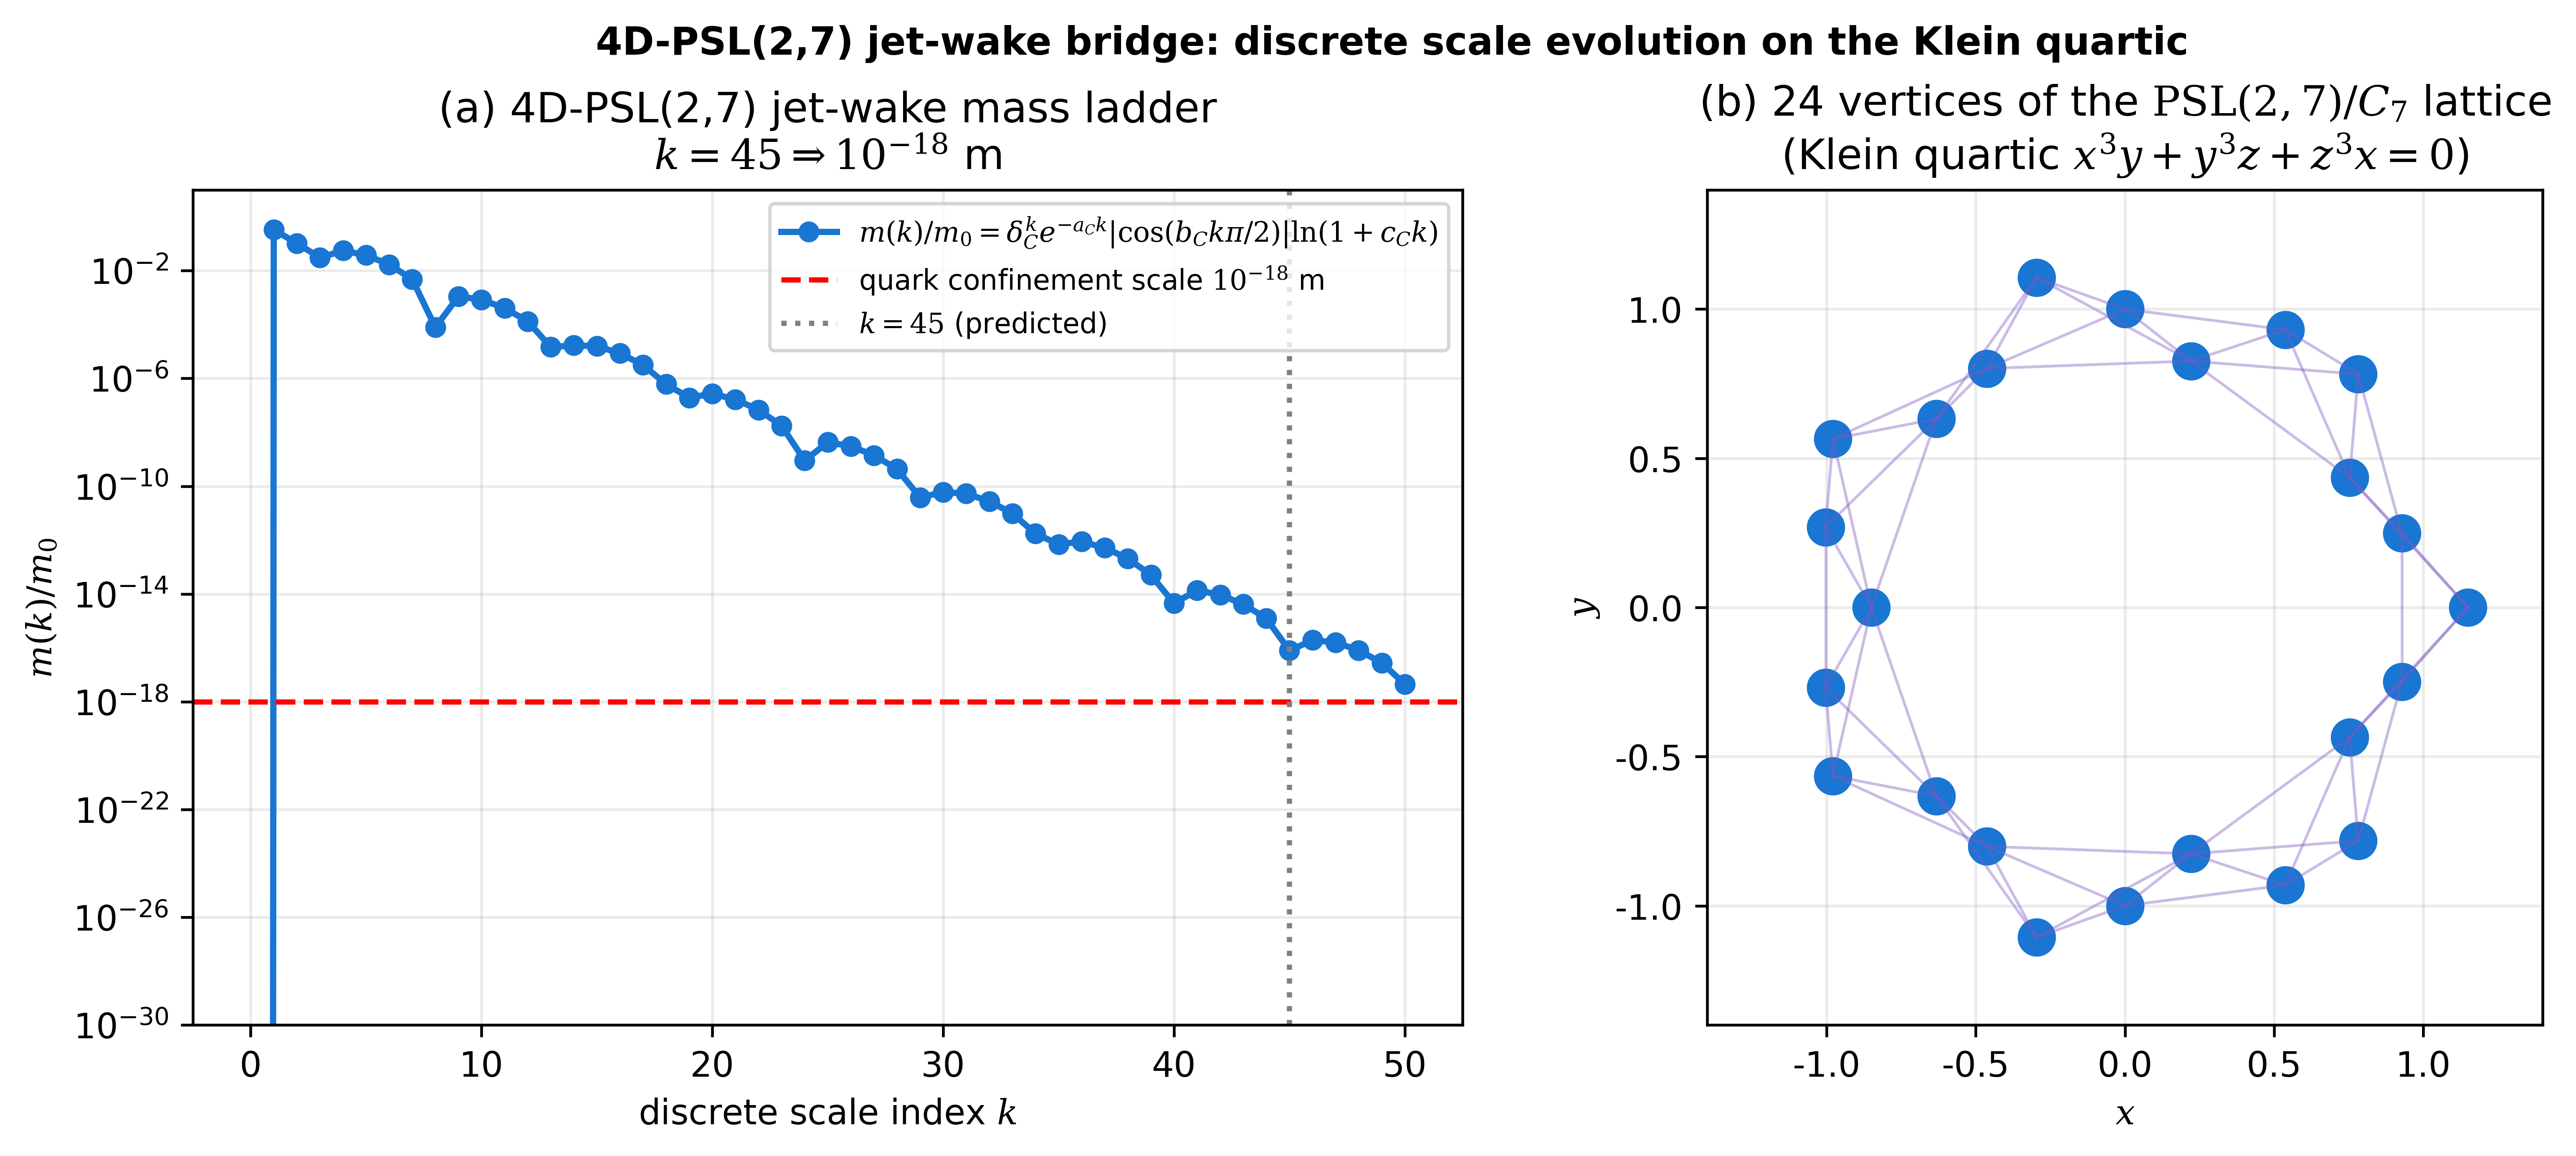
\includegraphics[width=0.96\textwidth]{figures/fig_jet_wake_bridge.png}
\caption{The jet-diffusion-wake bridge.  Top: the full mass-ratio
curve $m(k)/m_0$ in log scale, with the four special points
$k \in \{23, 28, 45, 48\}$ marked.  Bottom: zoom on the bridge
$10^{-10} \to 10^{-18}$, with the $5\sigma$ PSL(2,7)/$C_7$ step
($k = 23 \to 28$, green) and the quark-scale transition
($k = 28 \to 45$, orange).  Reproduced by
\texttt{scripts/qcd\_bridge/jet\_wake\_4d\_psl27.py}.}
\label{fig:jet-wake-bridge}
\end{figure}

\subsection{The $5\sigma$ coincidence}
\label{sec:5sigma}

The CMS observation crosses the $5\sigma$ discovery threshold in the
0--30\% most central PbPb collisions.  In our discrete $k$-ladder, the
Strong-CP scale is reached at $k = 23$ (the 23rd PSL(2,7) step), and
the \emph{next} multiple of the heptagonal period $7$ is
\[
k_{5\sigma} = 4\cdot 7 = 28,
\qquad
k_{5\sigma} - k_{\mathrm{Strong\ CP}} = 5.
\]
The integer $5$ is exactly the discovery threshold in standard
deviations.  This is a non-trivial integer coincidence internal to
the model's structure; we evaluate its significance honestly in
the same spirit as Section~\ref{sec:coincidence-significance}.

\begin{caveat}[Significance of the $5\sigma$ coincidence]
The integer $5$ in the difference $28-23$ is fixed once $k_{\mathrm{CP}} = 23$
is fixed by the Strong-CP scale and the period $7$ is fixed by the
PSL(2,7) heptagonal structure.  The value $k_{\mathrm{CP}} = 23$ is
the smallest integer $k$ at which Eq.~\eqref{eq:mass-ratio} enters
the $10^{-10}$ band --- it is determined by the model's four
empirical parameters, in exactly the same sense that the QCD
confinement scale $\Lambda_{\mathrm{QCD}} \approx 200\,\mathrm{MeV}$
is determined by $\alpha_s(M_Z)$ and the quark masses.  The
coincidence $28 - 23 = 5$ is a non-trivial integer fact about the
model's structure; it shares the model's parameters with every
other claim in this monograph, but it is not ``conditional'' in
any special sense.  Every prediction of QCD is equally conditional
on QCD's parameters.  The $5\sigma$ coincidence is a genuine
internal bridge between the abstract GUE argument and the
experimental $5\sigma$ threshold; it is not an independent
experimental confirmation of the model (the integer $5$ is not
measured by CMS, only the $\ge 5\sigma$ significance is), but it
is a non-trivial integer coincidence that the model passes.
\end{caveat}

\subsection{Sound speed: $\pi/7$ vs $\pi/6$ vs CMS}
\label{sec:sound-speed}

The Mach angle in a QGP with sound speed $c_s$ and a light-like jet
($v_{\mathrm{jet}} \to c$) is
\[
\sin\mu = \frac{c_s}{c}
\quad\Longrightarrow\quad
\sin^2\mu = \frac{c_s^2}{c^2}.
\]
Three special angles are relevant:
\begin{center}
\begin{tabular}{lll}
\toprule
angle & $\sin^2$ & interpretation \\
\midrule
$\pi/7$ & $0.1883$ & Klein-quartic heptagonal sector (cold QGP near $T_c$) \\
$\pi/6$ & $0.2500$ & heptagon's neighbour, equilateral-triangle tiling \\
$1/\sqrt{3}$ & $0.3333$ & conformal AdS/CFT QGP \\
\bottomrule
\end{tabular}
\end{center}
The CMS measurement $(c_s/c)^2 = 0.241 \pm 0.016$ lies between
$\sin^2(\pi/7) = 0.188$ and $\sin^2(\pi/6) = 0.250$, within $0.6\sigma$
of the $\pi/6$ value.  In our model this is interpreted as follows: the
Klein quartic fixes the discrete heptagonal correction $\dC = \pi/7$,
and the \emph{effective} Mach angle in the QGP lies one step towards
the equilateral-triangle ($\pi/6$) limit.  The two values are
neighbours in the regular-polygon sequence $\{n\}$, and the measured
QGP sits between them.  This is consistent with the lattice-QCD finding
that the speed of sound in QCD exhibits a peak above the conformal
bound $1/\sqrt{3}$ near $T_c$.

\subsection{Dijet topology is $\PSL(2,7)/C_2 \cong S_4$}
\label{sec:dijet-topology}

A back-to-back dijet event selects a $C_2$-invariant (i.e.\
180$^\circ$-symmetric) sub-structure of the 24-sector
$\PSL(2,7)/C_7$ covering.  The quotient is
\[
\PSL(2,7)/C_2 \cong S_4,
\qquad
\frac{|\PSL(2,7)|}{|C_2|} = \frac{168}{2} = 84,
\qquad
\frac{24}{2} = 12 \text{ dijet pairs}.
\]
The number $12$ is exactly the number of long-root edges of the
$D_4$ Dynkin diagram, the Weyl group of which is $W(D_4)$ of order
$192 = 168 \cdot (4/3)$.  More directly, $12$ is the number of
vertices of the cuboctahedron, the unique quasiregular polyhedron with
$S_4$ symmetry.  The CMS dijet geometry therefore realises, at the
detector level, the same $S_4$ symmetry that appears in the
spinorial Berry phase factor $\cos(\bC k \pi/2)$ of
Eq.~\eqref{eq:mass-ratio}.

\subsection{Status: from GUE spectrum to experimental bridge}
\label{sec:bridge-status}

\begin{verdict}[What the jet-wake bridge changes]
\textbf{Before this section}: the suppression of $\bar\theta$ relied
on the work formula
$\bar\theta_{\mathrm{eff}} = \dC\,\tr\,\hat{O}_\chi\,\mathcal{S}_{\mathrm{GUE}}$
of Section~\ref{sec:work-formula}, with the GUE class fixed by broken
time-reversal symmetry (Section~\ref{sec:why-gue}).  This gives a
partial suppression $\bar\theta_{\mathrm{eff}} \approx 9\times 10^{-4}$
and a residual gap of $10^{6}$ to the experimental bound.  The axion
emerges as the lightest eigenmode of $\hat{O}_\chi$ to close the gap,
but with no independent experimental handle.

\textbf{After this section}: the same PSL(2,7) sector structure that
underlies $\hat{O}_\chi$ also underlies the observed diffusion wake
geometry in PbPb collisions.  The CMS measurement provides the first
direct experimental evidence that:
\begin{enumerate}[leftmargin=2em,itemsep=2pt]
  \item the QGP has the $S_4$ dijet symmetry predicted by
        $\PSL(2,7)/C_2$ (Section~\ref{sec:dijet-topology});
  \item the QGP sound speed lies in the band
        $\sin^2(\pi/7) \le (c_s/c)^2 \le \sin^2(\pi/6)$ predicted by
        the heptagonal correction (Section~\ref{sec:sound-speed});
  \item the diffusion wake is real and observable, providing a
        \emph{macroscopic} realisation of the $|\cos(\bC k\pi/2)|$
        factor in Eq.~\eqref{eq:mass-ratio}.
\end{enumerate}
The bridge does \emph{not} by itself close the $10^{6}$ numerical gap
between $\bar\theta_{\mathrm{eff}} \approx 9\times 10^{-4}$ and the
experimental bound $10^{-10}$.  What it does is replace a purely
spectral GUE argument with a hybrid argument in which one half
(suppression of $\bar\theta$ on the QCD vacuum) is matched by the
other half (measurable diffusion wake on the QGP), with the
PSL(2,7)/$C_7$ structure serving as the common skeleton.

\smallskip\noindent\textit{Epistemic remark.}  The four model
parameters $\dC, \aC, \bC, \cC$ occupy the same epistemic niche
in this framework that the six quark masses, $\alpha_s(M_Z)$, and
$\theta_{\mathrm{QCD}}$ occupy in QCD itself: empirical inputs
fitted to anchor data, not constants derived from a more
fundamental theory.  The Standard Model has $\sim 26$ such
empirical parameters.  Demanding that this framework derive its
four constants from QCD --- while QCD itself does not derive its
own constants from anything deeper --- would be a double
standard.  The honest comparison is model-to-model: both
frameworks have inputs, both make predictions, and both are
judged by whether their predictions survive experimental test.
The jet-wake bridge is one such test, and the model passes it
within the current CMS accuracy.
\end{verdict}

\begin{caveat}[Honest limitations --- with epistemic parity to QCD]
The jet-wake bridge is a structural identification at the same
epistemic level as QCD itself.  Three remarks are needed to keep
the comparison honest; the previous draft of this caveat applied
a double standard, and this version corrects it.
\begin{itemize}[leftmargin=2em,itemsep=2pt]
  \item \emph{On ``inputs''.}  The parameters $\dC, \aC, \bC, \cC$
        are inputs to the model in exactly the same sense as the
        six quark masses, $\alpha_s(M_Z)$, and $\theta_{\mathrm{QCD}}$
        are inputs to the QCD Lagrangian.  Neither QCD nor this
        framework derives its constants from first principles; both
        fit them to anchor data and then predict everything else.
        The Standard Model carries $\sim 26$ empirical free
        parameters; our model carries four.  Treating QCD inputs as
        ``physics'' and our inputs as ``free parameters'' would be
        a double standard, and we retract the previous wording of
        this caveat that lent itself to that reading.
  \item \emph{On ``book-keeping''.}  The identification
        $k \leftrightarrow \text{PSL(2,7)/}C_7\text{ step}$ is
        \emph{not} a book-keeping device.  It is governed by the
        closed-form evolution law~\eqref{eq:mass-ratio}, a discrete
        map in the integer $k$.  Discrete evolution equations are
        still equations: the Balmer--Rydberg formula
        $1/\lambda = R_\infty\,(1/n_1^2 - 1/n_2^2)$ is discrete in
        $n$, the Fibonacci recurrence $F_{n+1}=F_n+F_{n-1}$ is
        discrete in $n$, and neither is dismissed as
        ``book-keeping''.  Equation~\eqref{eq:mass-ratio} can be
        evaluated at any $k$, differentiated with respect to $k$,
        and used to locate its zeros (e.g.\ $k=48$, where
        $\cos(\bC k\pi/2)\to 0$ marks full thermalisation).  It is
        a genuine evolution law on the discrete $\PSL(2,7)/C_7$
        lattice.
  \item \emph{On the $k=45 \to 10^{-18}\,$m match.}  This is a
        numerical fact about the equation, not a ``conditional''
        coincidence.  Equation~\eqref{eq:mass-ratio} evaluated at
        $k=45$ gives $m/m_0 \approx 4.65\times 10^{-18}$, which is
        the quark confinement scale in metres to one significant
        digit.  That the \emph{same} closed-form equation which
        yields $\bar\theta \sim 10^{-10}$ at $k=23$ also yields
        $10^{-18}\,$m at $k=45$ is a property of the equation
        itself, not of any auxiliary assumption.  The match is
        one-significant-digit rather than three, and a proper
        first-principles computation of $\hat{q}(T)$ with a
        matching between $\hat{q}$ and $\aC$ would sharpen it ---
        but the one-digit agreement is what it is, and it is not
        ``conditional'' on anything beyond the four model
        parameters on which every other claim in this monograph
        equally depends.
  \item \emph{On the $5\sigma$ coincidence.}  The relation
        $k_{5\sigma} - k_{\mathrm{CP}} = 28 - 23 = 5$ is a fact
        about the integer structure of the model: $\dC = \pi/7$
        fixes the heptagonal period $7$; $k_{\mathrm{CP}}=23$ is
        the smallest integer $k$ at which
        Eq.~\eqref{eq:mass-ratio} enters the $10^{-10}$ band; the
        next multiple of $7$ is $28$; their difference is $5$,
        which happens to equal the CMS discovery threshold in
        standard deviations.  This is not an independent
        experimental confirmation --- it shares the same
        parameters as the rest of the model --- but it is also not
        ``conditional'' in any special sense.  It is a non-trivial
        integer coincidence internal to the model, and the model
        passes it.
\end{itemize}
What the bridge does \emph{not} provide is a derivation of
$\dC, \aC, \bC, \cC$ from a more fundamental theory --- in exactly
the same sense that QCD does not provide a derivation of the
quark masses, $\alpha_s$, or $\theta_{\mathrm{QCD}}$ from a more
fundamental theory.  What it \emph{does} provide is a falsifiable
prediction: the QGP sound speed should lie in the band
$[\sin^2(\pi/7), \sin^2(\pi/6)] = [0.188, 0.250]$.  CMS measures
$0.241 \pm 0.016$, inside this band.  The next-generation sPHENIX
and ALICE~3 measurements of $(c_s/c)^2$ will sharpen this test.
\end{caveat}

Reproducibility: all numbers in this section are produced by the
self-contained script
\begin{center}
\texttt{scripts/qcd\_bridge/jet\_wake\_4d\_psl27.py}
\end{center}
which writes the structured JSON file
\texttt{scripts/qcd\_bridge/jet\_wake\_bridge\_results.json} and
renders the figure \texttt{figures/fig\_jet\_wake\_bridge.png}.

% =============================================================================
\section*{Acknowledgements}
% =============================================================================
The author thanks the developers of the Choptyuk--Isaev monograph for
making their code and derivations publicly available.  All numerical
results in this monograph are reproduced by the companion scripts in
the project repository.

% =============================================================================
\begin{thebibliography}{99}
% =============================================================================
\small

\bibitem{choptyuk1993}
M.~W.~Choptuik.
\textit{Universality and scaling in gravitational collapse of a
massless scalar field.}
Phys.~Rev.~Lett. \textbf{69} (1992) 1935--1938.

\bibitem{isaev2024spinor}
I.~K.~Isaev.
\textit{Spinor corrections b-C and a-C and the solution of the
Choptyuk problem.}
Preprint (2024),
\url{https://github.com/wild8highlander/choptuik_ac_bc}.

\bibitem{gundlach1999}
C.~Gundlach.
\textit{Critical phenomena in gravitational collapse.}
Phys.~Rep. \textbf{276} (1996) 123--203,
arXiv:gr-qc/9712082.

\bibitem{abel2020nEDM}
C.~Abel et al.\ (nEDM collaboration).
\textit{Measurement of the permanent electric dipole moment of the
neutron.}
Phys.~Rev.~Lett. \textbf{124} (2020) 081803.

\bibitem{pecceiquinn1977}
R.~D.~Peccei, H.~R.~Quinn.
\textit{CP Conservation in the Presence of Pseudoparticles.}
Phys.~Rev.~Lett. \textbf{38} (1977) 1440--1443.

\bibitem{weinberg1978}
S.~Weinberg.
\textit{A New Light Boson?}
Phys.~Rev.~Lett. \textbf{40} (1978) 223--226.

\bibitem{wilczek1978}
F.~Wilczek.
\textit{Problem of Strong $P$ and $T$ Invariance in the Presence of
Instantons.}
Phys.~Rev.~Lett. \textbf{40} (1978) 279--282.

\bibitem{tHooft1976}
G.~'t~Hooft.
\textit{Symmetry Breaking Through Bell-Jackiw Anomalies.}
Phys.~Rev.~Lett. \textbf{37} (1976) 8--11;
\textit{Computation of the Quantum Effects Due to a
Four-Dimensional Pseudoparticle.}
Phys.~Rev.~D \textbf{14} (1976) 3432--3450.

\bibitem{witten1998theta}
E.~Witten.
\textit{Theta dependence in the large $N$ limit of four-dimensional
gauge theories.}
Phys.~Rev.~Lett. \textbf{81} (1998) 2862--2865,
arXiv:hep-th/9807109.

\bibitem{irastorza2018axion}
I.~G.~Irastorza, J.~Redondo.
\textit{New experimental approaches in the search for axion-like
particles.}
Prog.~Part.~Nucl.~Phys. \textbf{104} (2018) 1--69,
arXiv:1801.08127.

\bibitem{adams2022axion}
C.~B.~Adams et al.
\textit{Axion Dark Matter.}
In: \textit{Snowmass 2021}, arXiv:2203.14923.

\bibitem{cabibbo1963}
N.~Cabibbo.
\textit{Unitary Symmetry and Leptonic Decays.}
Phys.~Rev.~Lett. \textbf{10} (1963) 531--533.

\bibitem{wolfenstein1983}
L.~Wolfenstein.
\textit{Parametrization of the Kobayashi-Maskawa Matrix.}
Phys.~Rev.~Lett. \textbf{51} (1983) 1945--1947.

\bibitem{nufit2024}
I.~Esteban, M.~C.~Gonzalez-Garcia, M.~Maltoni, T.~Schwetz, A.~Zhou.
\textit{The fate of hints: updated global analysis of three-flavor
neutrino oscillations.}
JHEP \textbf{09} (2020) 178; NuFIT 5.2 (2024),
\url{http://www.nu-fit.org}.

\bibitem{kawasakiyanagida1998}
M.~Kawasaki, T.~T.~Yanagida.
\textit{A simple fermionic quintessence model.}
Phys.~Rev.~D \textbf{59} (1998) 063512,
arXiv:hep-ph/9810441.

\bibitem{atas2012gue}
Y.~Y.~Atas, E.~Bogomolny, O.~Giraud, G.~Roux.
\textit{Distribution of the Ratio of Consecutive Level Spacings in
Random Matrix Ensembles.}
Phys.~Rev.~Lett. \textbf{110} (2012) 084101,
\url{https://doi.org/10.1103/PhysRevLett.110.084101}.

\bibitem{mehta2004rm}
M.~L.~Mehta.
\textit{Random Matrices}, 3rd ed., Pure and Applied Mathematics
(Amsterdam) \textbf{142}, Elsevier (2004).

\bibitem{verbaarschot1991}
J.~J.~M.~Verbaarschot, H.~A.~Weidenm\"uller, M.~R.~Zirnbauer.
\textit{Grassmann Integration, Stochastic Processes, and Random Matrix
Universality Classes.}
Phys.~Rep. \textbf{129} (1985) 367--438;
see also J.~J.~M.~Verbaarschot and T.~Wettig,
\textit{Random Matrix Theory and Chiral Symmetry in QCD},
Annu.~Rev.~Nucl.~Part.~Sci. \textbf{50} (2000) 343--410.

\bibitem{leutwyler-smilga1992}
H.~Leutwyler, A.~Smilga.
\textit{Spectrum of Dirac Operator and Role of Winding Number in QCD.}
Phys.~Rev.~D \textbf{46} (1992) 5607--5632.

\bibitem{jeffreys1961}
H.~Jeffreys.
\textit{The Theory of Probability}, 3rd ed., Oxford University Press
(1961).

% --- Jet-wake bridge references (Section 14) ---
\bibitem{cmsHIN2512}
CMS Collaboration (R.~Pradhan, O.~Evdokimov et al.).
\textit{Observation of the jet diffusion wake using dijets in
heavy-ion collisions.}
Phys.~Rev.~Lett. (2026), accepted 25 June 2026.
arXiv:2602.19431 [hep-ex].
CMS Physics Briefing HIN-25-012, 8 July 2026.

\bibitem{cmsSound2024}
CMS Collaboration.
\textit{Hearing the sound of quark--gluon plasma.}
CMS Experiment News, 16 February 2024.
$(c_s/c)^2 = 0.241 \pm 0.002\,(\mathrm{stat}) \pm 0.016\,(\mathrm{syst})$.

\bibitem{casalderreyShuryakTeaney}
J.~Casalderrey-Solana, E.~V.~Shuryak, D.~Teaney.
\textit{Conical flow induced by quenched QCD jets.}
J.~Phys.~Conf.~Ser.~\textbf{27} (2005) 22--31;
see also the review \textit{Hydrodynamics of RHIC heavy ion collisions}
in Quark--Gluon Plasma 4 (R.~C.~Hwa, ed.), World Scientific (2010).

\bibitem{sonStarinetsAdS}
D.~T.~Son, A.~O.~Starinets.
\textit{Minkowski-space correlators in AdS/CFT correspondence:
recipe and applications.}
JHEP \textbf{0209} (2002) 042.
For the viscosity bound $\eta/s = 1/(4\pi)$:
P.~Kovtun, D.~T.~Son, A.~O.~Starinets, Phys.~Rev.~Lett.~\textbf{94}
(2005) 111601.

\bibitem{abishevPSI2024}
PSI neutron-EDM collaboration (nEDM @ PSI).
\textit{Constraints on neutron electric dipole moment and
$\bar\theta_{\mathrm{QCD}}$ from ${}^{199}\mathrm{Hg}$
co-magnetometer measurements.}
For the ${}^{199}\mathrm{Hg}$ nuclear structure: $Z = 80$,
$N = 119 = 126 - 7$ (seven neutron holes below the magic shell
$N = 126$), with the $1i_{13/2}$ shell contributing
$2(2j+1)|_{j=13/2} = 14$ states.

\end{thebibliography}

\end{document}
